%%%%%%%%%%%%%%%%%%%%%%%%%%%%%%%%%%%%%%%%%%%%%%%%%%%%%%%%%%%%%%%%%%%%%%%%%%%%%%%
%% Tutorial                                                                  %%
%%%%%%%%%%%%%%%%%%%%%%%%%%%%%%%%%%%%%%%%%%%%%%%%%%%%%%%%%%%%%%%%%%%%%%%%%%%%%%%
\chapter[Tutorial: Net type and application] {Complete Tutorial:\\
  Net type and Application}
\label{chap:tutorial}

In this chapter, we discuss an example, which goes through the complete
development process of a new Petri net type and an application for the ePNK.
This serves as a tutorial which comes across all major aspects of the ePNK.
In order to cover some more interesting aspects of the ePNK, we have
chosen a slightly artificial Petri net type, which we call \emph{technical
Petri net type}. This technical Petri net type are classical Place/Transition
Systems (P/T-systems)\footnote
  {In a P/T-system a marking of a place may have multiple tokens.}
with with three additional features: \emph{read arcs}, \emph{inhibitor arcs}
and \emph{reset arcs}. The ePNK application is a simple simulator for this
net type.

As usual a \emph{read arc} just check whether their is a token on the attached
place, but does not change the marking of this place; an \emph{inhibitor arc},
by contrast, checks that there is no token on the attached place, but also does
not change the marking when the transition fires. A \emph{reset arc} does not
have any influence on the enabledness of the transition, but when it fires, all
tokens from places attached to the transition with a reset arc, are removed.

Actually, in our \emph{technical Petri net type}, a \emph{reset arc} does not
directly run from a place to a transition, but from a \emph{page} to a
\emph{transition}. Then, all places contained in that page will be reset
(i.\,e.\ all tokens will be removed) when the transition fires. In combination
with using reference places, this reset of a page allows us to reset larger
parts of a Petri net with a single reset arc which avoids cluttering the net
with too many reset arcs.

We discuss this net type and the application from the end-user's point of
view in Sect.~\ref{sec:tutorial:tool}. In
Sect.~\ref{sec:tutorial:concepts}, we discuss
the conceptual idea of how to realize this application with the ePNK; at last, in
Sect.~\ref{sec:tutorial:technical}, we discuss the major
technical steps to actually implement the application. This also covers
the respective modelling and code generation steps, necessary configurations,
and possible pitfalls and problems with the Eclipse tools and Eclipse IDE-- and
even the installation of the ePNK and EMF. All the code of that example is
available online and we recommend that you install the example in your
\emph{development workspace} while working through the technical steps of this
tutorial; which is discussed in Sect.~\ref{sec:tutorial:technical}.

\section{The tool}
\label{sec:tutorial:tool}

Figure~\ref{fig:tutorial:app1} shows a screenshot of our example tool that we
are going to develop in this tutorial as an extension of the ePNK.
Figure~\ref{fig:tutorial:app1} shows the graphical editor of the ePNK with a
Petri net of the new \emph{technical Petri net type} that we use for this
tutorial. The net is shown in the graphical editor of the ePNK (actually, you
can see the net's two pages). We use Fig.~\ref{fig:tutorial:app1} for briefly
explaining the features of this \emph{technical net type}. After that, we also
briefly discuss the features of the simulator.

\subsection{The technical net type}
\label{sec:tutorial:tool:nettype}

Figure~\ref{fig:tutorial:app1} shows all the features of the \emph{technical net
type}. First of all, there are the standard concepts of Petri nets, such as
\emph{places}, \emph{transitions} and \emph{arcs} and the \emph{initial marking}
of places (indicated by a \emph{label} attached to the \emph{place}, which
defines the number of \emph{tokens} on that \emph{places} initially). Moreover,
there are the additional concepts of \emph{pages} and \emph{reference nodes},
which are coming from the PNML \cite{HKea09} or its ePNK implementation. See
Sect.~\ref{sec:intro:PNML} for details.
The example net shown in Fig.~\ref{fig:tutorial:app1} consists of two
\emph{pages}, $pg_1$ on the left and $pg_2$ on the right. Page $pg_2$ is
actually a sub-page of $pg_1$ indicated by the large rounded rectangle shown on
$pg_1$; the contents of page $pg_2$ is shown in the graphical editor open on he
right-hand side.
Note that all the elements, which graphically appear to be inside the
rounded rectangle representing page $pg_2$ on page $pg_1$ are actually objects
of page $pg_1$; they are just arranged in such a way that they appear to be
inside page $pg_2$. The only elements contained in $pg_2$ are the
\emph{reference places} shown on the right-hand side. These reference
places, however, refer to the places $p_2$, $p_3$, $p_4$, $p_5$ and $p_7$ of the
page $pg_1$.
This is not directly visible in the graphical representation reference places;
but you can see in the properties view that the reference place with id
$rp_5$ (and name $p_7$) actually refers to the place $p_7$ on page $pg_1$. So we
use the graphical alignment of the places $p_2$, $p_3$, $p_4$, $p_5$
and $p_7$ ``inside'' the rounded rectangle to put emphasize on this relation,
since it has meaning for the effect of the attached reset arc, which we discuss
later.

\begin{sidewaysfigure}[p!!]
  \centerline{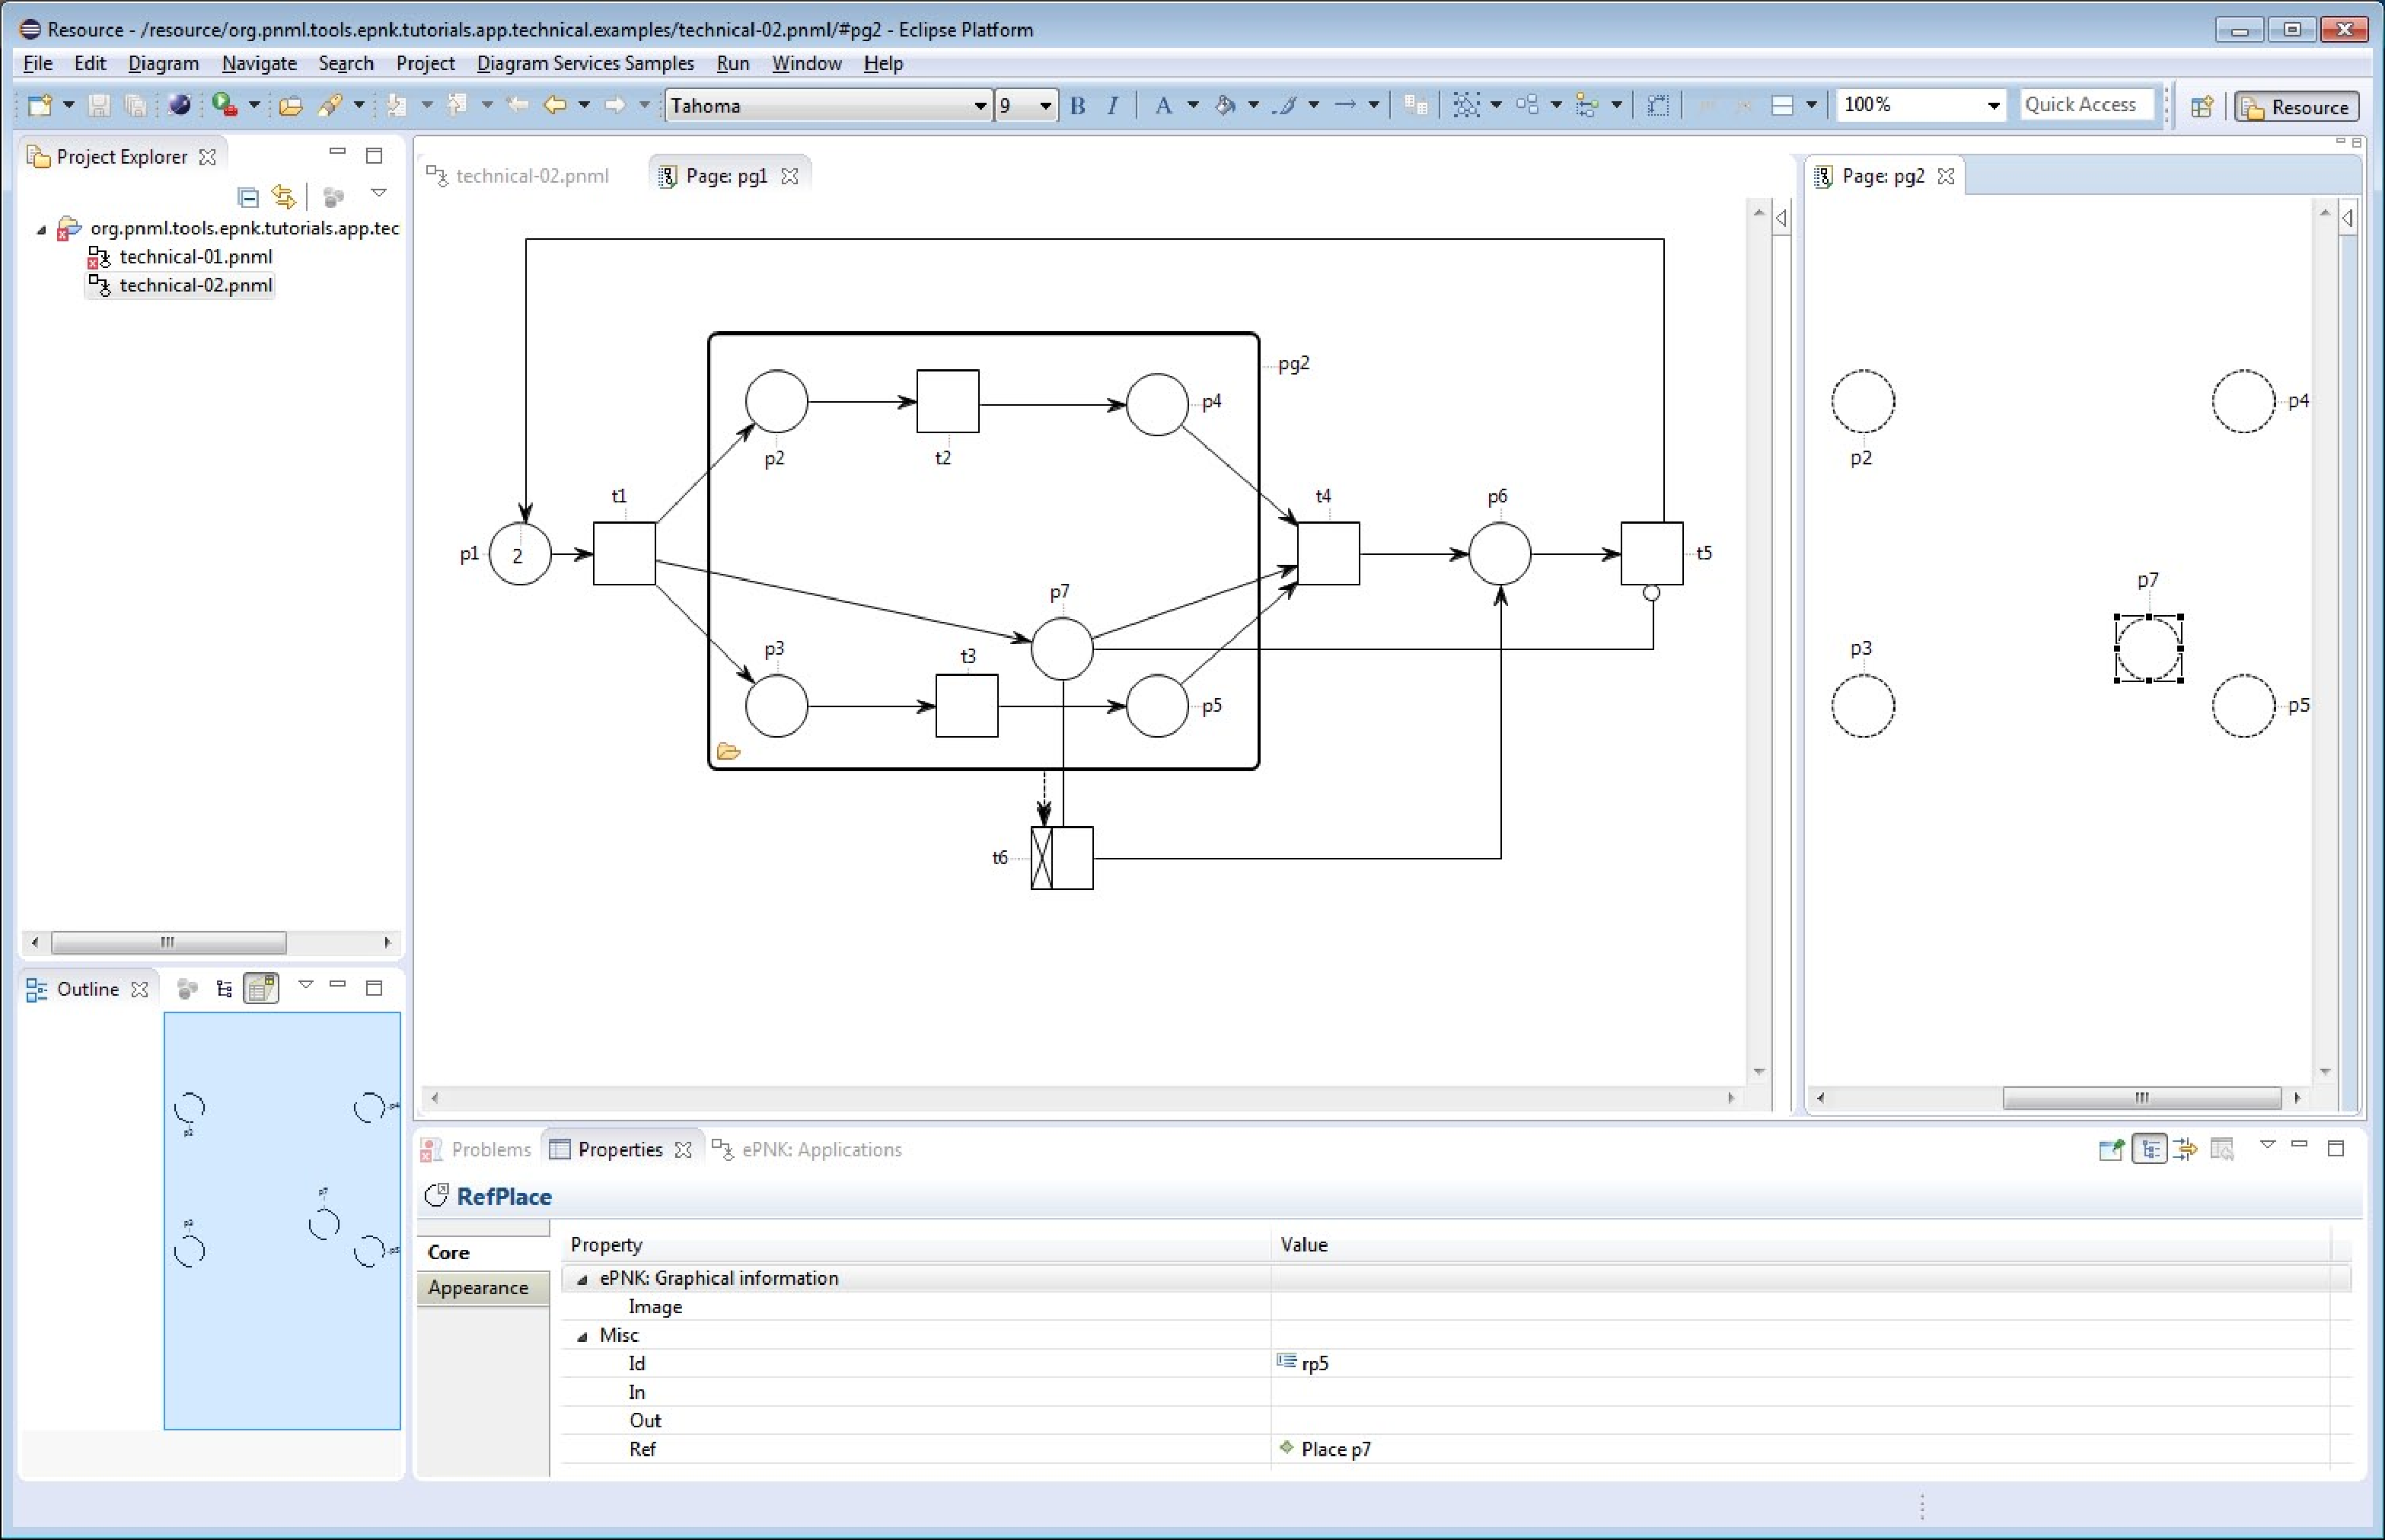
\includegraphics[scale=.34]{tutorial/TechnicalApplication1.pdf}}
  \caption{The example tool with an example of a technical net}
  \label{fig:tutorial:app1}
\end{sidewaysfigure}

In the \emph{technical net type}, we can connect \emph{places} and
\emph{transitions} with \emph{normal} arcs. As usual \emph{normal} arcs can run
from a place to a transition or the other way round. In addition, there are two
other kinds of arcs, which run from a place to a transition: \emph{read} arcs
and \emph{inhibitor} arcs. As the name suggest, a \emph{read} arc will not
change the number of tokens on the attached place; but the attached
transition can fire only, when there is at least on token on the place attached
to the other end of the read arc.
The inhibitor also does not change the number of tokens on the attached place when the transition fires. But, by contrast to the read
arc, the transition will only be allowed to fire, if there is no token on the
attached place (a token on the attached place ``inhibits'' the firing of the
transition). A \emph{read} arc is graphically represented as a line without
arrow heads on either end, but it technically runs from a place to a
transition. In our example, there is only one \emph{read} arc, running from
place $p_7$ to transition $t_6$.
An \emph{inhibitor} arc is graphically represented with a ``lollipop''
decoration at the transition end --  and the direction of the arc is from
the place to the transition. In our example, there is only one \emph{inhibitor}
arc, running from place $p_7$ to transition $t_5$.

The concepts discussed so far are all well-know concepts in Petri nets. We
will see later, that in our simulator for \emph{technical net type}, the
end-user is able to deactivate \emph{read} arcs and \emph{inhibitor} for some
simulation step -- ignoring the \emph{deactivated} arcs. There is one additional
concept in our \emph{technical net type}: these are \emph{reset} arcs, which --
just for the fun of it -- run from a page to a transition. In our example, there is one
\emph{reset} arc running from page $pg_2$ to transition $t_7$. A reset arc
does not have any effect on the enabledness of the attached transition; but,
when the transition fires, the tokens from all places contained in the attached
page will be removed. To be more precise, the tokens will be removed from the
places contained on the page and from the places to which the \emph{reference
places} on that page refer to (we say that the \emph{reference place}
\emph{resolve} to that \emph{place}).
In our example, these are the places $p_2$, $p_3$, $p_4$, $p_5$ and $p_7$ again. Graphically,
a \emph{reset} arc is represented by a dashed line with a double arrowhead.
The dashed line indicating that this arc does not prevent the transition from
firing; the double arrow head indicating that all tokens will be
removed from the places on that page.

At last, there is a minor twist\footnote
  {To be honest, we have chosen this feature only in order to demonstrate how
   to customize the graphical appearance of net objects in this tutorial.},
which is only of graphical nature. The
graphical representation of transition $t_7$ shows a cross in the left third of the
rectangle representing the transition. This indicates that this
transition does not have any \emph{normal} arc running to it. Since this
situation is sometimes not desired, it is indicated with a
special graphics; likewise, if there is no \emph{normal} arc starting at
the transition, this is graphically represented by a cross in the right
third of the transition. 

\subsection{The application}
\label{sec:tutorial:tool:application}

In addition to realizing a new net type, which then can be created and edited
in the graphical editor of the ePNK, the ePNK allows adding
\emph{application} on Petri nets. The applications could be some
analysis, simulation or verification; and the applications can visualize which
their results with a graphical feedback to the end-user, on top of the graphical
representation in the graphical ePNK editor.

In this tutorial, we discuss how to develop a \emph{simulator} for our
\emph{technical net type}, which we had introduced in
Sect.~\ref{sec:tutorial:tool:nettype}. In the following, we discuss this
simulator and its features from the end-user's point of view.

When a net or actually a page of a net of some type is open in the graphical
editor of the ePNK (and when this editor has the focus), all applications that
are defined for this net can be started by selecting the application in a small
drop down menu in the \emph{ePNK applications view}, which is indicated by
a small red circle in Fig.~\ref{fig:tutorial:app2}. In this figure, the
simulator called \emph{Technical Simulator (Tutorial)} was started already;
once started, some overlays in the graphical overlay indicate the initial
marking of the net, and also the enabled transition are highlighted. The
current marking of the net in the simulator is shown by a blue number to
the top-right of the respective place; but only places which have at least
one token hav such an annotation. This annotation for a place is also called
a \emph{marking} of the place -- to be precise, it is the \emph{current
marking} of the place -- as opposed to the \emph{initial} one which is
represented in the net itself. In Fig.~\ref{fig:tutorial:app2}, place $p_1$ has
two tokens; all the other places do not have a marking. The \emph{enabled}
transitions in the current marking are highlighted with a red overlay --
in the example, only transition, $t_1$, is enabled.

\begin{figure}[hbtp!!]
  \centerline{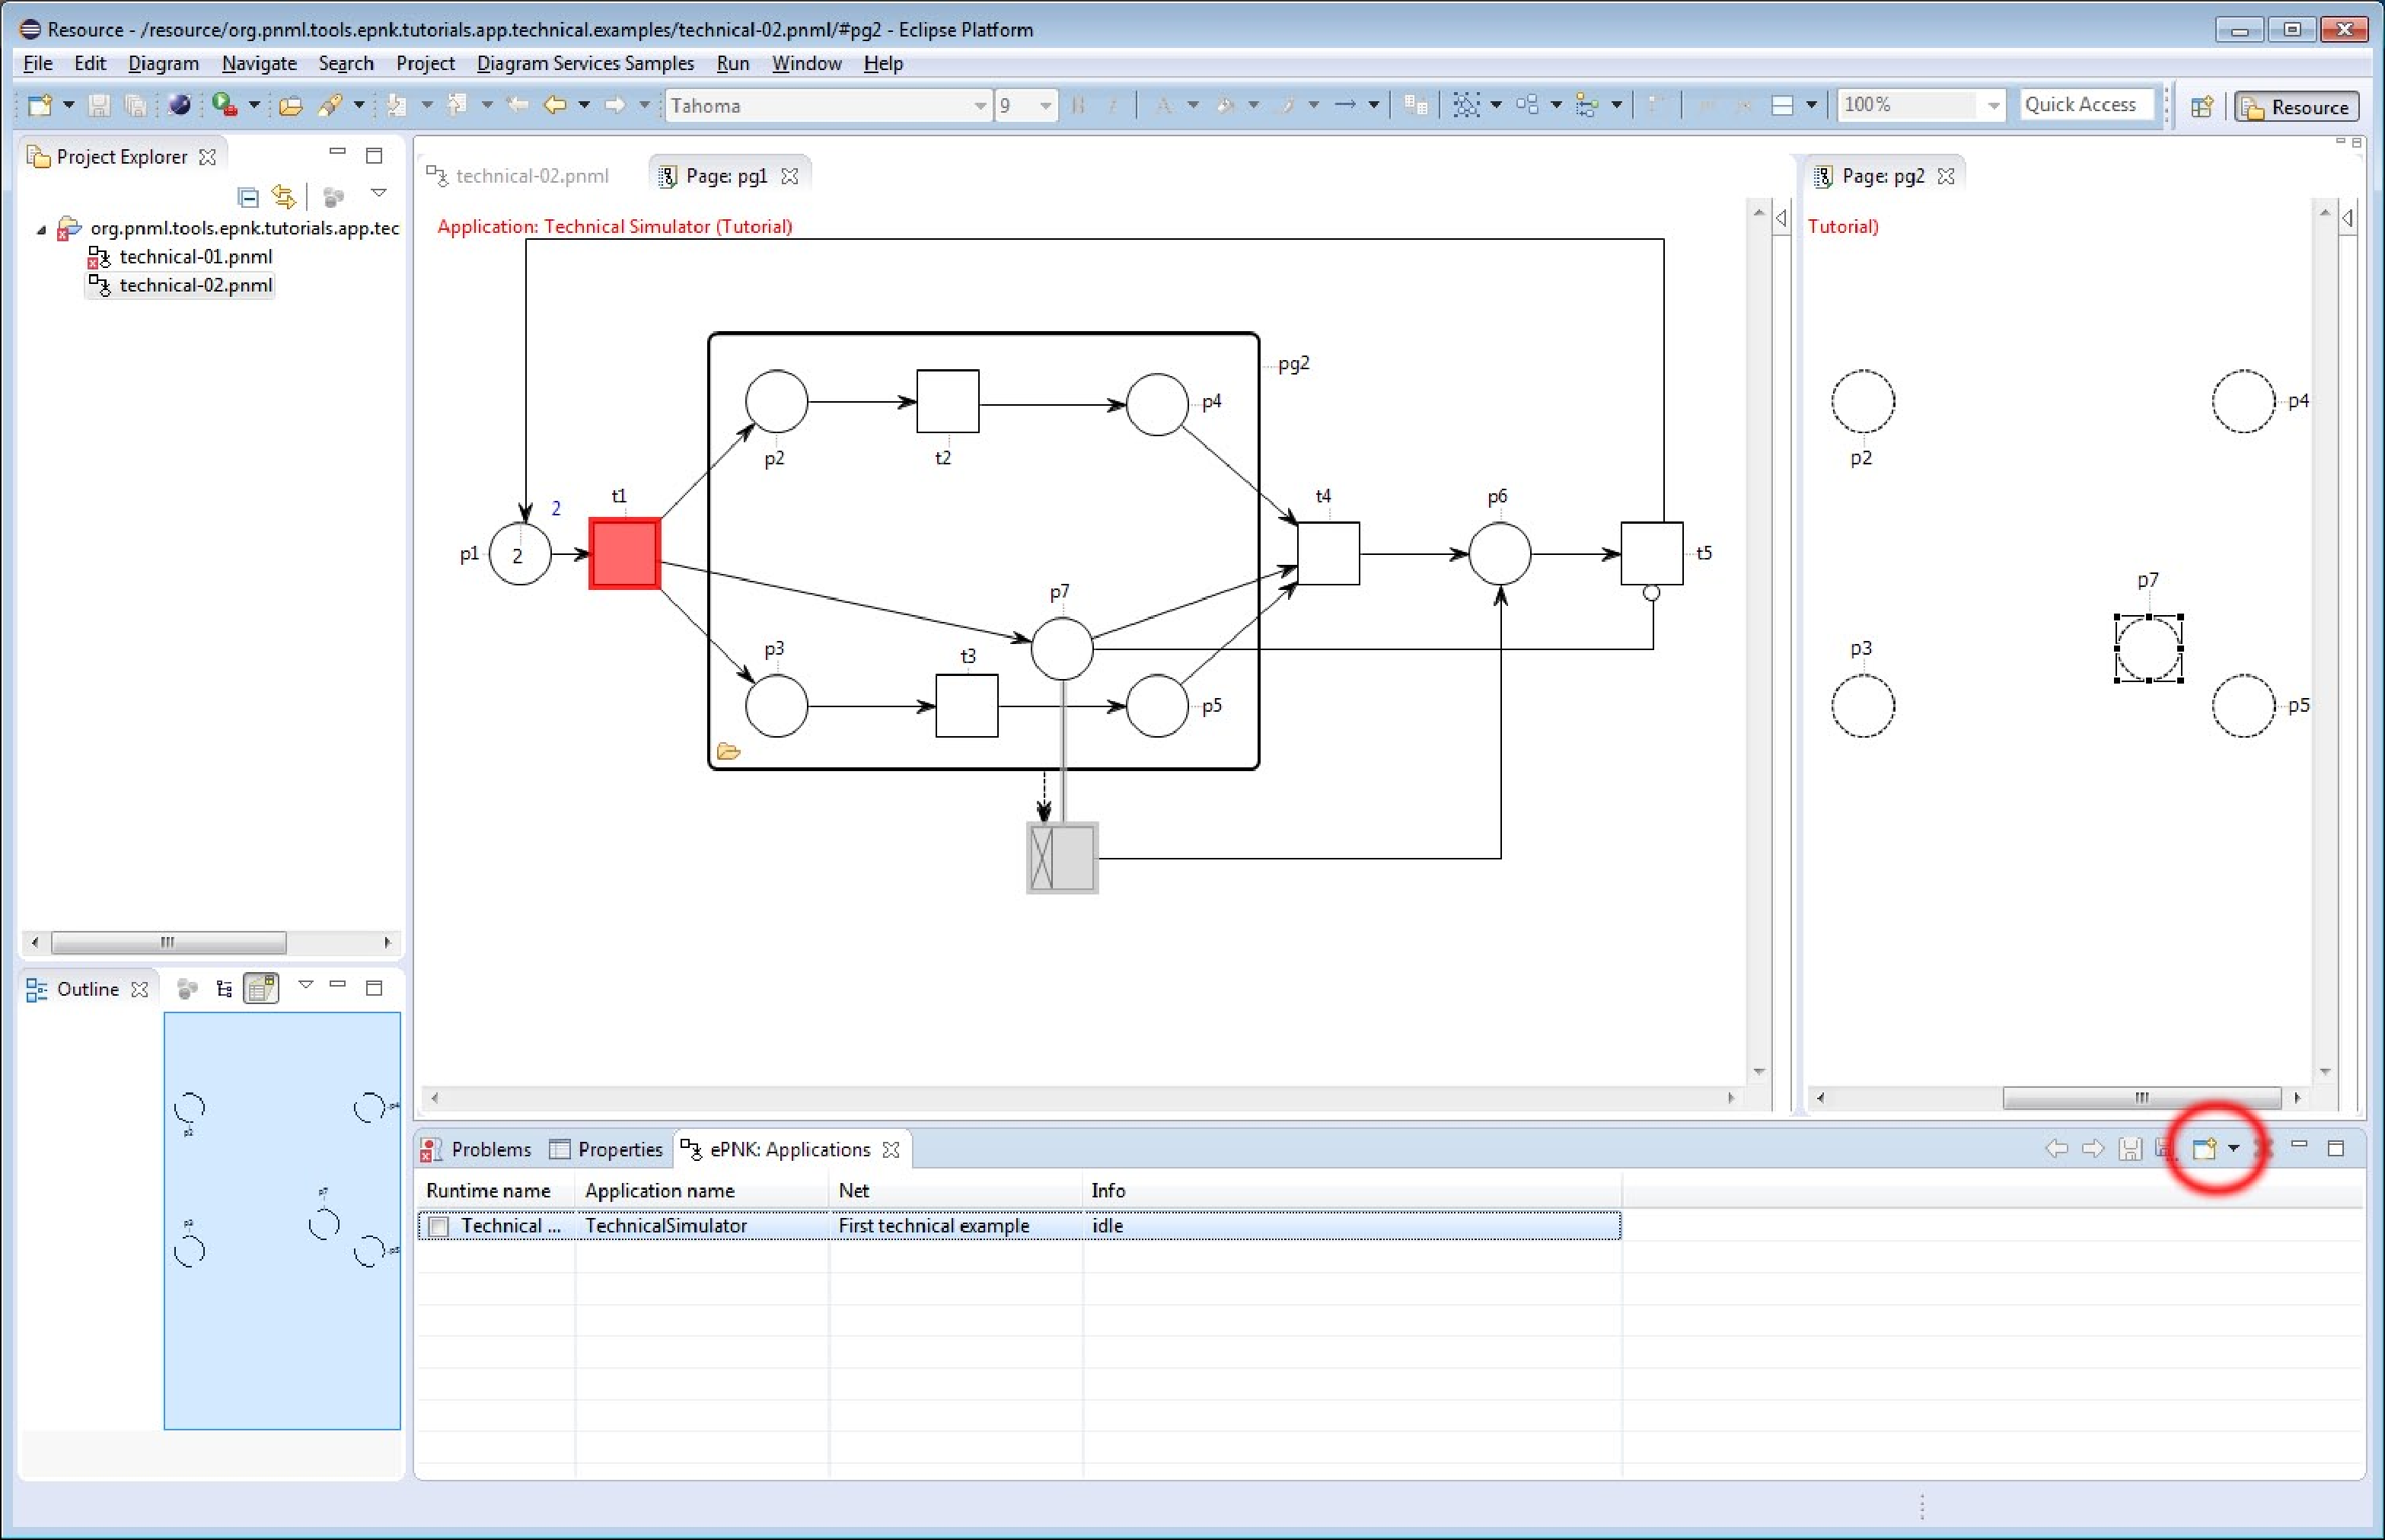
\includegraphics[scale=.24]{tutorial/TechnicalApplication2a.pdf}}
  \caption{The example net with the example simulator started}
  \label{fig:tutorial:app2}
\end{figure}

Note that, in the situation of  Fig.~\ref{fig:tutorial:app2}, also transition
$t_6$ at the bottom is highlighted with some light grey overlay and also
the read arc to place $p7$ has a light grey overlay. This indicates that, when
ignoring read and inhibitor arcs, transition $t_6$ would be enabled. We say
that this transition is \emph{weakly enabled}. By clicking on the read arc,
the end-user could choose to ignore that arc and then fire the transition. We
discuss that later.

When double-clicking on an \emph{enabled transition}, the respective transition
will \emph{fire}, the \emph{marking} of the places will change and the
\emph{enabled} transitions in the new marking will be highlighted. Figure~\ref{fig:tutorial:app3} shows
the situation after the end-user has fired (double-clicked on) the sequence
of transitions $t_1$, $t_1$, $t_2$, $t_3$, and $t_4$. In that situation, places
$p_2$, $p_3$, $p_7$ and $p_6$ have one token each (have \emph{marking} $1$), and
transitions $t_2$,  $t_3$, and $t_6$ are \emph{enabled}. Transition $t_5$ is
only \emph{weakly enabled} since the inhibitor arc from place $p_7$ to
transition $t_5$ prevents it from firing (place $p_7$ has a token).

In Fig.~\ref{fig:tutorial:app3}, you can also see another detail of the
simulator: the current marking is not only shown as an annotation of the
respective place. It is also shown as annotation of each reference place
that \emph{resolves to} the place -- as you can see for the reference places
shown on the right-hand side.
 
\begin{figure}[p!!]
  \centerline{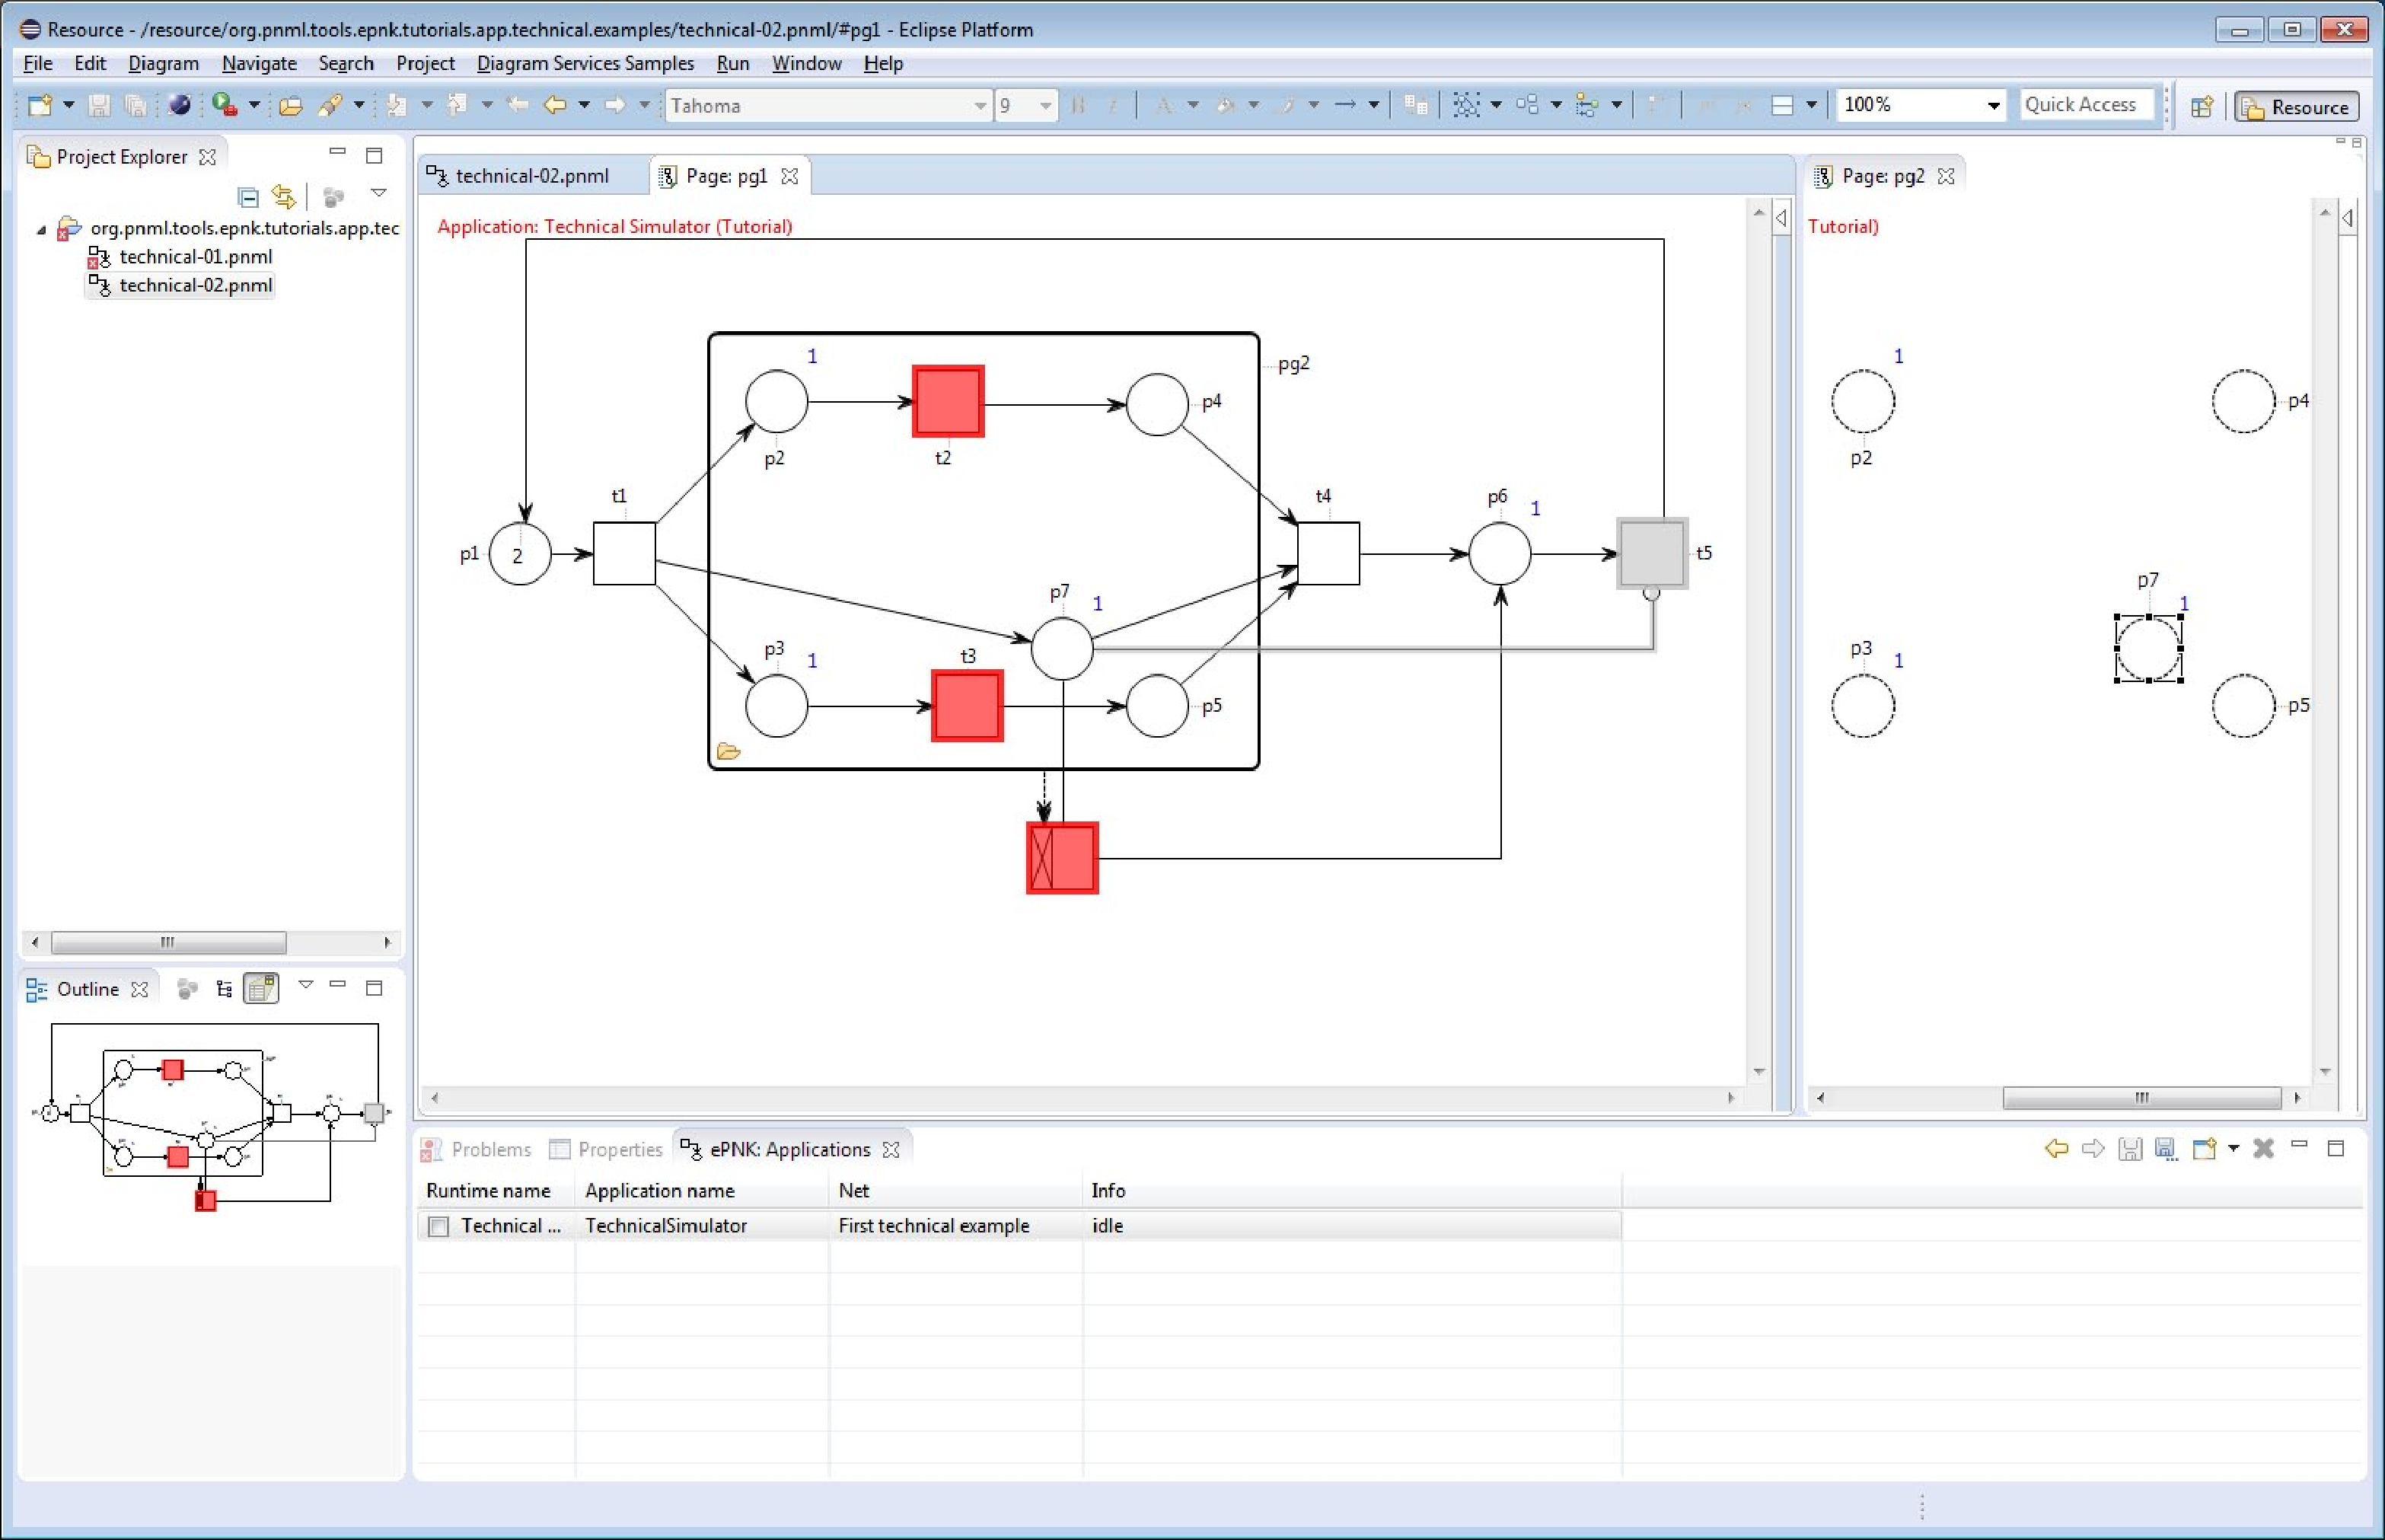
\includegraphics[scale=.24]{tutorial/TechnicalApplication3.pdf}}
  \caption{The simulator after firing transition $t_1$, $t_1$,
  $t_2$, $t_3$ and $t_4$}
  \label{fig:tutorial:app3}
\end{figure}

\begin{figure}[p!!]
  \centerline{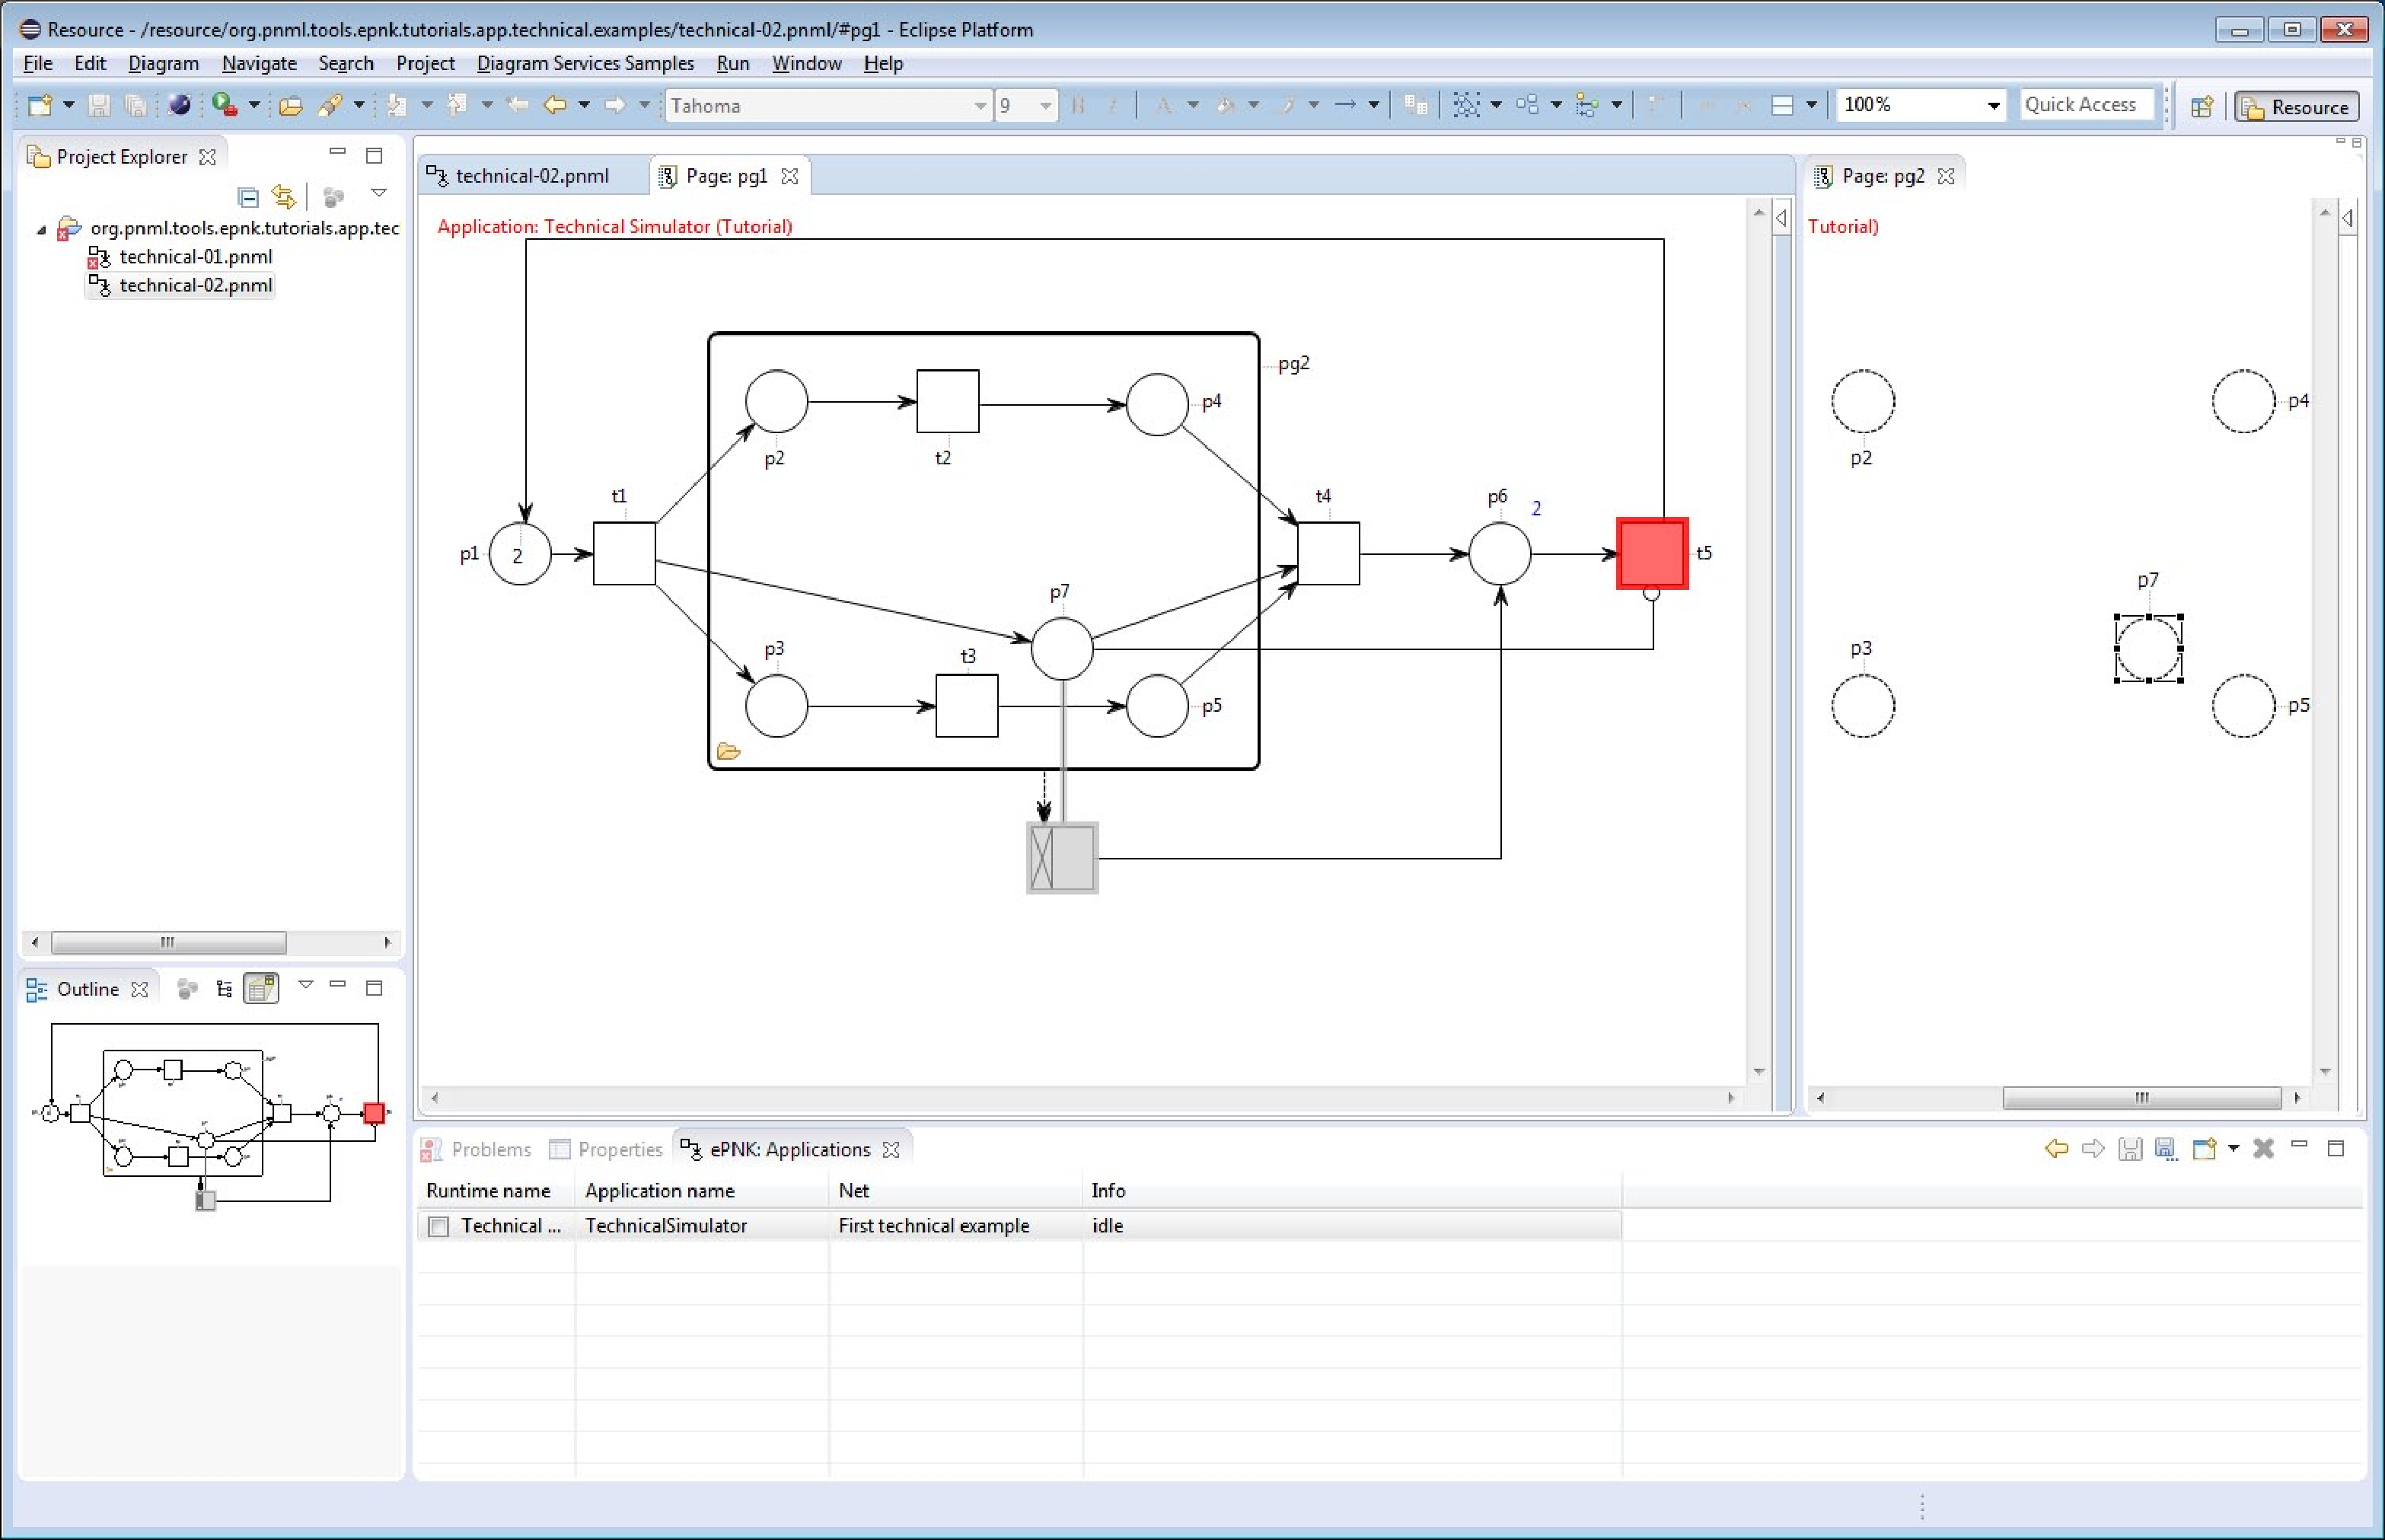
\includegraphics[scale=.24]{tutorial/TechnicalApplication4.pdf}}
  \caption{The simulator after additionally firing $t_6$}
  \label{fig:tutorial:app4}
\end{figure}

Figure~\ref{fig:tutorial:app4} shows the situation after \emph{firing}
transition $t_6$. Since this transition has a reset arc from page $pg_1$
all tokens are removed from the respective places on that page. The only
place that has tokens now is place $p_5$: it has two tokens now since
transition $t_6$ added another token.  Transition $t_5$ is enabled now,
since there is no token on place $p_7$ anymore. Moreover, transition $t_6$ is
weakly enabled.


Let us come back to the notion of a \emph{weakly enabled} transition, which is
a transition that would be enabled when ignoring conditions imposed by
\emph{read} arcs and \emph{inhibitor} arcs. In our example in Fig.~\ref{fig:tutorial:app4},
the bottom transition $t_6$ is weakly enabled only since the place at the
other end of the \emph{read} arc, place $p_7$ does not have a token. This
is indicated by the light-grey overlay of the transition and of the read arc.

The speciality of our technical net simulator is that the end-user can
deactivate \emph{read} arcs and \emph{inhibitor} arcs, by clicking on them.
Deactivated arcs will be shown with a red overlay. Once all \emph{read} arcs and
\emph{inhibitor} preventing the enabledness of a transition are
\emph{deactivated}, the transition will be enabled, indicated by a red overlay
again. Figure~\ref{fig:tutorial:app5} shows the effect of the end-user clicking
on the read arc in the situation of Fig.~\ref{fig:tutorial:app4}.
Then, the end-user can double-click on it and fire it.

\begin{figure}[hbtp!!]
  \centerline{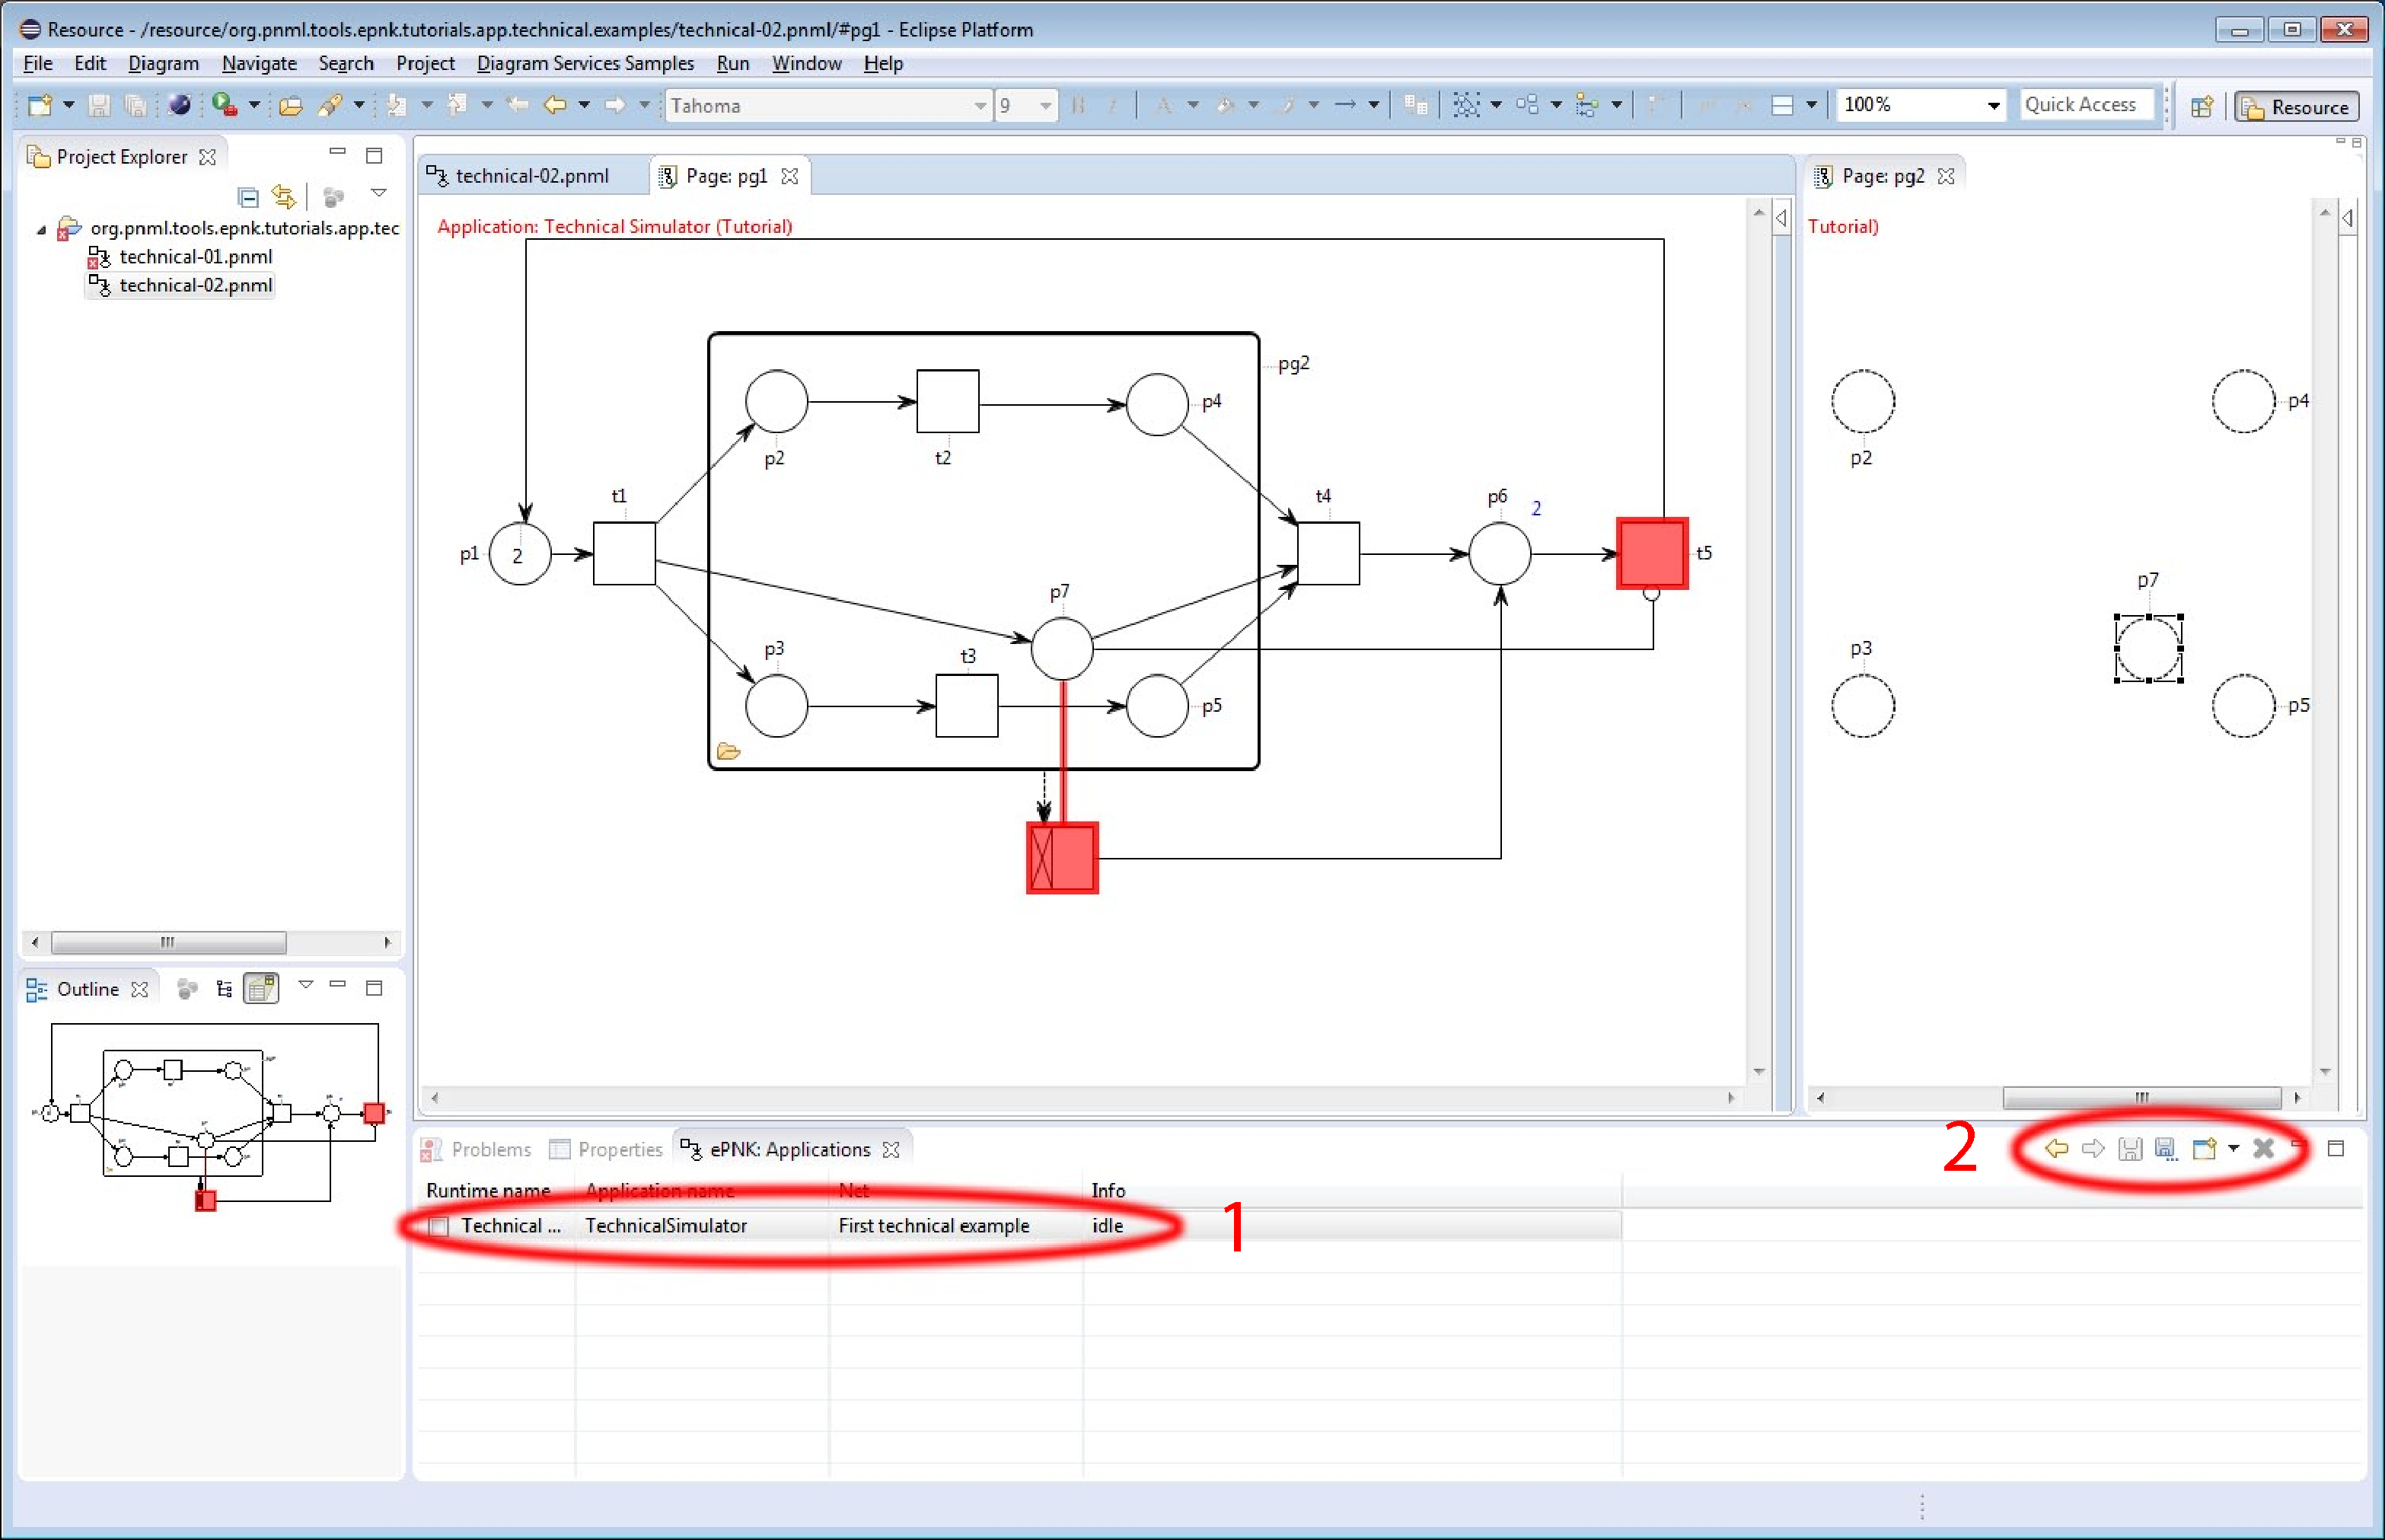
\includegraphics[scale=.24]{tutorial/TechnicalApplication5a.pdf}}
  \caption{The simulator after deactivating the read arc}
  \label{fig:tutorial:app5}
\end{figure}

At last, let us have a look at some standard features of the ePNK and the
application view. The application view shows a list of all the ePNK applications currently
running in the ePNK on some net. In the situation shown in
Fig.~\ref{fig:tutorial:app5}, only one application is running. The end-user can
select one of the running applications or un-select all applications. Then, the
visual feedback from the selected application is shown in the graphical editor
of the respective net. The end-user can also delete (shut down) applications
by selecting the check boxes of the respective applications (see line marked by
1 in Fig.~\ref{fig:tutorial:app5}) and clicking on the delete button (which
 will turn red once at least one application is selected) in the ePNK
 applications view (see the part marked with 2 in Fig.~\ref{fig:tutorial:app5}).

Note that there are also some other buttons  (see the part that is marked with 2
in Fig.~\ref{fig:tutorial:app5}). The \emph{back} and  \emph{forward} buttons
allow the end-user to go back and forth in the simulation, the disk buttons 
allows the end-user to save the current state the and firing sequence of the
simulator to a file.
Such a \emph{saved state of an application} can be loaded again, when starting
a new application with ``Load application'' in the start application
drop down menu.

\section{Conceptual steps}
\label{sec:tutorial:concepts}

In this section, we discuss the conceptual steps for realizing the tool which we
had discussed in Sect.~\ref{sec:tutorial:tool}.
The first step is the definition of our \emph{technical Petri net type}, which
basically consists of a class diagram capturing the concepts of our \emph{technical Petri net type}
and some constraints. The second step is the definition of the graphical
appearance of the features our \emph{technical Petri net type} -- in our case
the arcs and the transitions. The last step is the definition of the
\emph{simulator application} for our \emph{technical Petri nets}.

Note that, in this section, we do not discuss any technical details, how to
create the models, how to generate the code, or how to plug in the
extensions to the ePNK in order not to loose track of the overall picture.
The technical details are discussed in Sect.~\ref{sec:tutorial:technical}.

\subsection{Petri net type}
\label{subsec:tutorial:concepts:pnt}

In this section, we present a class diagram (actually an Ecore diagram),
which reflects the extensions of our \emph{technical Petri net type} as
discussed in Sect.~\ref{sec:tutorial:tool:nettype}. Basically, the extension
on top of the basic net elements, \emph{places}, \emph{transitions}, and
\emph{arcs}, are that arcs can be of kind \emph{normal}, \emph{read},
\emph{inhibitor} and \emph{reset}. In addition, places can have an
\emph{initial marking}, indicating how many tokens are on each place
initially.

\subsubsection{Petri net type definition}
\label{subsubsec:tutorial:concepts:pntd}

Figure~\ref{fig:tutorial:concepts:pntd} shows the class diagram with all the
features of our \emph{technical Petri net type}, which is called a \emph{Petri
net type definition} or \emph{PNTD} for short. This diagram refers to some classes which
are defined by the ePNK in the \emph{PNML core model}: these are the classes
shown in magenta on the left and on the top of the diagram. The other classes
shown in light cream are the definition of our \emph{technical Petri net type},
which extend the concepts of the \emph{PNML core model}.

\begin{sidewaysfigure}[hbtp!!]
  \centerline{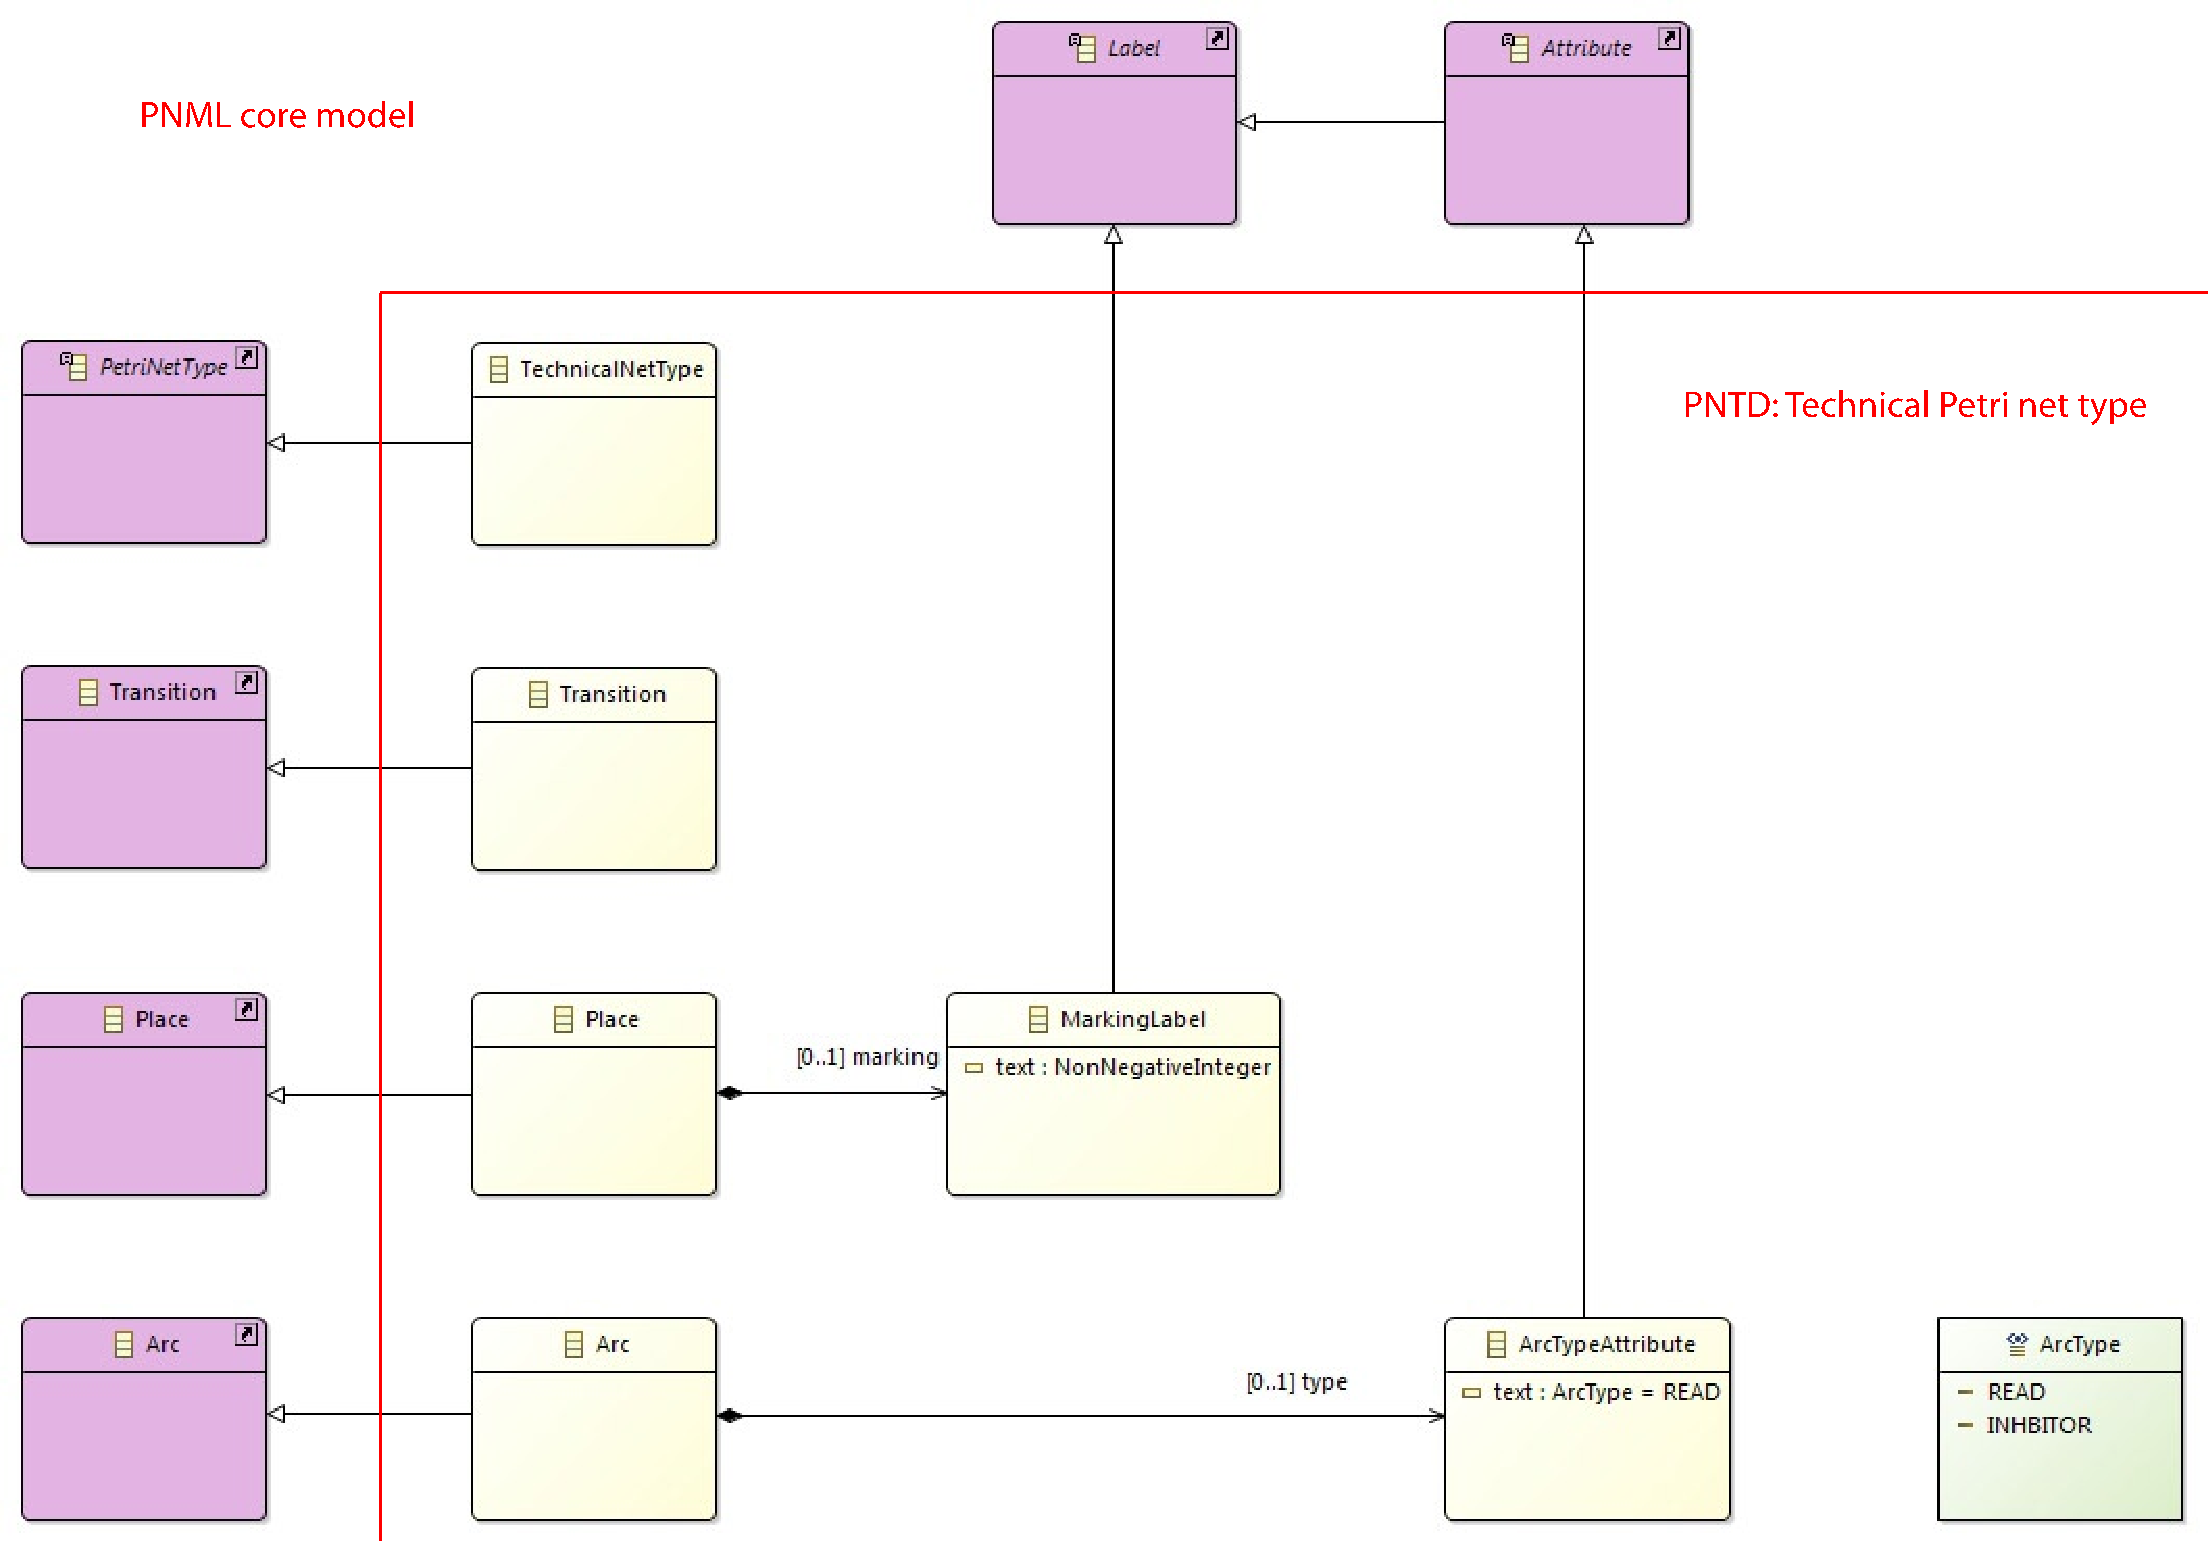
\includegraphics[scale=.45]{tutorial/technical-nets-pntd-2.pdf}}
  \caption{The Petri net type definition for the technical Petri net type}
  \label{fig:tutorial:concepts:pntd}
\end{sidewaysfigure}

There are two major extensions in our Petri net type definition in
Fig.~\ref{fig:tutorial:concepts:pntd}, the \emph{arc} and \emph{place}. Both
extend the respective concept of the PNML core model. Arcs have a concept of
\emph{ArcTypeAttribute} with an attribute \emph{text} of the enumeration type
\emph{ArcType}, which is also defined in this PNTD. \emph{Places} have
a \emph{MarkingLabel} with an attribute \emph{text} of the type
\emph{NonNegativeInteger}, which is a data type defined in the PNML core model.

The class \emph{ArcTypeAttribute} extends the class \emph{Attribute} from the
PNML core model, and the \emph{MarkingLabel} extends the class  \emph{Label}
from the PNML core model. This defines how the ePNK should handle these
additional features. A label will be graphically represented as an annotation
to the respective element. In our example, the initial marking is shown as such
a textual annotation (see Fig.~\ref{fig:tutorial:app1}) ``2'' inside the place,
this label however could be freely moved by the end-user. The type attribute
for places is not shown as an annotation of the arc; it is represented by the
graphical representation of the respective arc. It can be edited by the end-user
in the properties view, once the respective arc is selected.

Note that the classes \emph{ArcTypeAttribute} and \emph{MarkingLabel} are
associated with the class \emph{Arc} or \emph{Place} with a composition. The
name of this composition, will be the name of the respective feature and its
cardinality says how many of these features each element can have. In our
case, both cardinalities are $[0..1]$, which means that the feature is
optional and there can be at most one.

You might have realized the the enumeration \emph{ArcType} does have two
literals only: \emph{READ} and \emph{INHBITOR}. At a first glance, this might
look awkward since in the discussion of our technical Petri net type we
mentioned four different types: \emph{normal}, \emph{read}, \emph{inhibitor} and
\emph{reset}. The reason is that the arc type feature is optional, and that we
interpret a missing or not set arc type feature as \emph{normal}. Likewise
\emph{reset} is the default (or actually only) interpretation for arcs
running from a page to a transition. Therefore, it is enough that the
enumeration \emph{ArcType} represents \emph{READ} and \emph{INHBITOR}, which are
the only ones the end-user needs to set explicitly.

Note that also the \emph{marking} feature is optional. If the marking feature
is not set, the default interpretation is $0$.

In the diagram from Fig.~\ref{fig:tutorial:concepts:pntd}, there are two
additional classes defined: \emph{Transition} and \emph{TechnicalNetType},
both of which do not define any extensions on top of the PNML core model
classes they inherit from. The class \emph{Transition} would actually not be
necessary, since in our technical net type transitions do not have any
extensions. But introducing an explicit class for transitions in our PNTD allows
us to explicitly to refer to the transitions of this type. The class
\emph{TechnicalNetType}, however, is necessary: it represents the net type we
define here, and we will need it later to plug in the extension to the ePNK.

\subsubsection{Constraints}
\label{subsubsec:tutorial:concepts:constraints}

The diagram of Fig.~\ref{fig:tutorial:concepts:pntd} defines the additional
concepts of our technical Petri net type. But, is is not precise enough since
it would allow arcs running from a transition to a place to be an inhibitor
arc, which we do not want. Actually, without additional restrictions, arcs
could run between all kinds of nodes, for example between two places or between
two transitions; arcs would be even be allowed to run between two pages.

Therefore, we need to define an additional constraint that forbid arcs that
our technical net type should not have. We define an OCL constraint for
that purpose. 

\begin{figure}[htbp!]
\lstinputlisting[label=lst:tutorial:concepts:pntd:ocl,language=OCL,tabsize=2,stringstyle=\small,%
caption={OCL constraint for arcs}]%
  {code/tutorial/arc-ocl.txt}
\end{figure}

Listing~\ref{lst:tutorial:concepts:pntd:ocl} shows this  OCL constraint for
arcs: it states that an \emph{Arc} of or our technical net type can
have three different forms:
\begin{enumerate}
  \item It can run from a place to a transition. Since there also can
        be arcs between reference nodes of that kind, the requirement
        is slightly generalized to \emph{PlaceNode} and \emph{TransitionNode}.
        In that case there is no restriction of the arc's type.
        
  \item It can run from a transition to a place. For the same reasons as
        above, the requirement is slightly more general: the arc can run
        from a \emph{TransitionNode} to a \emph{PlaceNode}. For arcs from
        a transition to a place, however, the arc's type should not be set
        (i.\,e.\ it must be a \emph{normal} arc).
        
  \item It can run from a page to a transition, slightly more generalized to
        run from a \emph{Page} to a \emph{TransitionNode}. Also in that case,
        the arc's type should not be set. In this case, the arc is interpreted
        as a \emph{reset} arc.
\end{enumerate}

In order to demonstrate that constraints can also be defined in
Java, we actually introduce our example has one additional constraint: there
should not be duplicate read or inhibitor arcs between the same two nodes.
The implementation of \emph{Java constraints}, however, will first be discussed
in the technical details section (see
Sect.~\ref{subsubsec:tutorial:technical:constraints:java}).

\subsection{Graphics of the Petri net type definition}
\label{subsec:tutorial:concepts:graphics}

In Sect.~\ref{sec:tutorial:tool:nettype}, we have discussed already that some
features of our technical Petri net type should be graphically visualized in
a particular way. The type of an arc should be indicated by a dedicated
graphics for \emph{read}, \emph{inhibitor} and \emph{reset arcs} (see
Fig.~\ref{fig:tutorial:app1}). It is actually quite typical that Petri net
objects which have an attribute extension, also have a dedicated graphics for
that type of Petri net object; the reason is that the value of an attribute
is visible only in the properties view of the tool when the object is
selected, but not in the graphical representation of the net itself, unless
there is a dedicated graphical representation for it.

In our technical Petri net type, we have chosen to have a dedicated graphics
for transitions, too: transitions with no ingoing normal arc or no outgoing
should be indicated with a cross in the left or right third of the transition,
respectively, as shown for transition $t_6$ in Fig.~\ref{fig:tutorial:app1}. 

For each type of net object with a dedicated graphics, we need to implement a
\emph{Figure} class, which takes responsibility for the graphics of that
element.
Basically, there are two ways of implementing the such figures. The
first one is to change the figure by changing its configuration and graphical
attributes. In our example, we use that way for the graphical representation of
arcs. The second one is to override how the figure is actually drawn.
In our example, we use that way for the graphical representation of transitions.


Listing~\ref{lst:tutorial:concepts:graphics:arc} shows the code snippet which
configures how an arc is drawn, dependent on its type. Basically, there are
four cases: if the arc is a \emph{read} arc, both the source and the target
decorator are set to {\tt null}, so that the arc does not have any arrow
head; if the arc is an \emph{inhibitor} arc the source decorator is set to
{\tt null} and the target decorator is set to a new \emph{CircleDecoration}
which is a class provided with the ePNK; for a \emph{reset} arc, the line style is
set to dashed, and the target decorator is set to a new
\emph{DoubleArrowHeadDecoration}; at last, for normal arcs the line style is
solid, there is no source decorator, and the target decorator is a normal
\emph{ArrowHeadDecoration}, which is provided by the ePNK. If need should be,
new decoration classes could be implemented for the graphical extension. But,
this is not necessary in our tutorial example.

Note that Listing~\ref{lst:tutorial:concepts:graphics:arc} gives just a glimpse
of the respective class. We discuss more details on how to plug in this class
and how and when to properly update the graphical representation of a net object
in the technical details.

\begin{figure}[htbp!]
\lstinputlisting[label=lst:tutorial:concepts:graphics:arc,language=Java,tabsize=2,stringstyle=\small,%
caption={Arc graphics: defining appearance of acs}]%
  {code/tutorial/arc-graphics-java.txt}
\end{figure}


Listing~\ref{lst:tutorial:concepts:graphics:transition} shows the code snippet
which takes care of drawing the graphical representation of a transition --
overriding the \emph{fillShape} method. On top of drawing the figure as usual
by calling {\tt super.fillShape(graphics)}, the two conditional statements
are code for ``drawing'' the separator and a cross in the left respectively right
third of the transition using the programming mechanisms of Eclipse Draw2D, if
necessary. Also here, there are some more technical details on how to plugin the
respective class to the ePNK and how to update the graphics when needed. We
discuss this in the technical details.

\begin{figure}[htbp!]
\lstinputlisting[label=lst:tutorial:concepts:graphics:transition,language=Java,tabsize=2,stringstyle=\small,%
caption={Transition graphics: drawing the figure}]%
  {code/tutorial/transition-graphics-java.txt}
\end{figure}

\subsection{The simulator application}
\label{subsec:tutorial:concepts:app}

At last, we need to define the simulator application, which allows the end-user
to simulate the technical nets, and which visualizes the current state of
the Petri net and the currently enabled transitions graphically on top
of the net shown in the graphical editor.

\subsubsection{Runtime annotations}
\label{subsubsec:tutorial:concepts:app:annot}

In order to separate concepts from the actual graphical representation, the
ePNK allows us to define \emph{annotations} for nets, which reflect runtime
information for our application. In our case, this would be the current state of
the simulator, information on the enabled transitions and activated and deactivated
arcs.

Like for the definition of a Petri net type, the conceptual annotations of
an application can be defined by a class diagram, which extends some basic
annotation concepts provided by the ePNK.
Figure~\ref{fig:tutorial:concepts:app:annot:model} shows this model, where
the two classes shown on the top and in magenta represent the based concepts
from the ePNK: \emph{object annotations} is any form of annotation of any
Petri net object; \emph{textual annotations} is information that typically
is represented by a text instead of a graphical overlay.

The classes represented in light cream are the \emph{annotations} needed for our
simulator.
\emph{EnabledTransition} is an annotation for weakly enabled
transition -- the value of attribute \emph{enabled} indicates whether 
the transition is \emph{truly} enabled. \emph{Marking} represents the
current marking of a  place (i.e.\ the number of tokens on that place). The
actual value is represented by its attribute \emph{value}. Since the value
should be shown as textual annotation, this class extends not only the
\emph{ObjectAnnotation} but also \emph{TextualAnnotation} of the ePNK.

At last \emph{InvolvedArc} is an annotation for arcs, which indicate arcs
of a weakly enabled transition that prevent the enabledness of this
transition. This way, the end-user can toggle whether the arc is \emph{active}
or not. The status of this user's selection is represented by attribute
\emph{active}.

In order to keep track of the arcs involved in an enabled transition, there
are two compositions from \emph{EnabledTransition} to \emph{InvolvedArc}: one
for the transition's incoming arcs and one for the outgoing arcs (the outgoing
arcs are actually not used in our example). This way, it is possible to navigate
between enabled transition annotations and the involved arc annotations.

Note also that there is a bidirectional relationship between the
\emph{EnabledTransition} itself. The reason is that a single transition can have
many reference transitions referring to it. In our simulator, also the
reference transitions that resolve to an enable transition should be marked as
enabled. The reference \emph{resolve} represents the transition, the reference
\emph{ref} represents all the reference transitions. We will see later in more
detail how our simulator uses this information.

\begin{figure}[hbtp!!]
  % \centerline{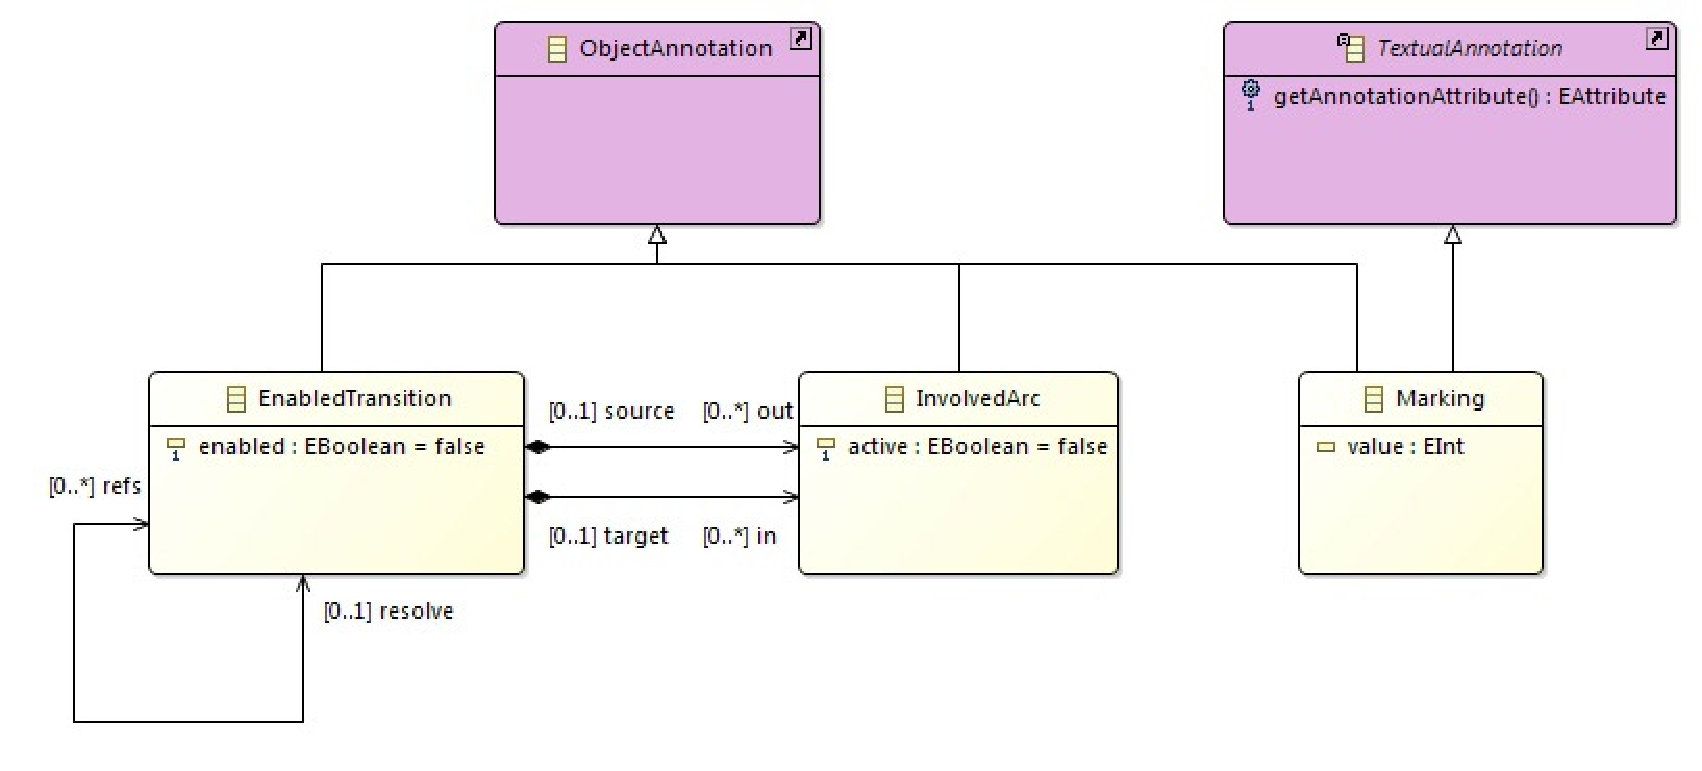
\includegraphics[scale=.45]{tutorial/techsimannotations.pdf}}
  \centerline{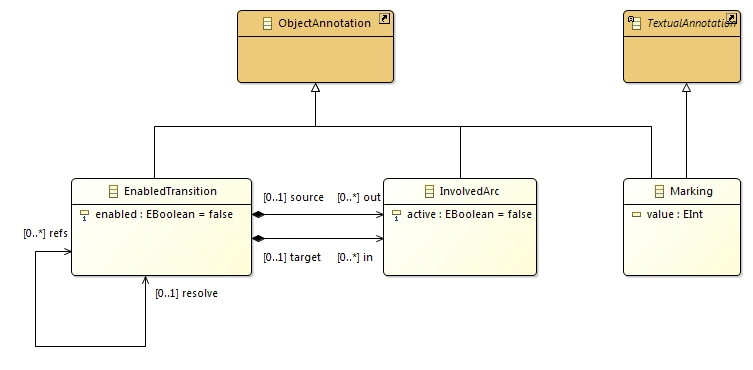
\includegraphics[scale=.45]{tutorial/techsimannotations.jpg}}
  \caption{Simulator: annotations model}
  \label{fig:tutorial:concepts:app:annot:model}
\end{figure}

An \emph{PNK application}, basically, consists of a list of
\emph{net annotations}, each of which which in turn consists of some
\emph{object annotations}.
Moreover, there always is a \emph{current} net annotation, which for example
represents the current state of the simulator. In our example, a net annotation represents
the current markings of the places plus the enabled transitions and the involved
arcs and their state.

In order to visualize the current state of an ePNK application in the graphical
editor, an ePNK application uses one or more \emph{presentation handlers}. A 
\emph{presentation handler} tells, for each annotation, how it should be
visualized in the net.
In order for end-user to be able to interact with the simulator via
the annotations, an ePNK application uses one ore more \emph{action
handlers}.
An \emph{action handler} defines how the simulator should react to a user interaction (mouse
press, mouse release, and mouse double click). This could for example, be
firing a transition by updating the net annotations, or toggling the active status 
of an involved arc. We discuss more details in the technical parts of
this tutorial.

Here we briefly discuss the main ingredients and functionality that
needs to be implemented for our simulator (and actually most kinds of
simulators):
\begin{enumerate}
\item We need some data structure or dedicated class, which represents 
      a \emph{marking of the net}, which basically is a mapping from places to
      integers.
\item We need a method, which computes the \emph{initial marking of the net}
      from a net model.
\item We need methods, which, for a given marking and some transition, computes
      whether the transition is \emph{enabled}, and which are the \emph{involved
      arcs}.
\item We need a method which for a given marking and a given enabled transition
      computes the marking which is the result after \emph{firing the
      transition in the given marking}. 
\item We need a method, which from a marking \emph{computes a net annotation}.
      representing the marking of the places as well as the enabled transitions,
      and the involved arcs.
\end{enumerate}

We discuss in the technical steps how the above methods can be combined
into a complete simulator using also the presentation handlers and action
handlers.

\section{Technical steps}
\label{sec:tutorial:technical}

In Section~\ref{sec:tutorial:concepts}, we have discussed the major conceptual
steps for realizing a Petri net type definition (PNTD) for our technical net
type and simulator for them based on the ePNK.

In the following sections, we discuss all the technical details, some subtle
issues concerning tooling, and possible problems that might occur on the way,
and how to deal with them. We start with some installation information in
Sect.~\ref{sec:tutorial:technical:install} and how to install the project
implementing the extensions discussed in this tutorial in your Eclipse workspace.
Then, we go through the steps which we discussed in
Sect.~\ref{sec:tutorial:concepts} in some more detail, discussing the models and
the source code of the Eclipse projects.

Note that the tricky issues and problems are sometimes not in the resulting
projects, models or code, but in how to actually create, configure, and
manipulate them. Therefore, we also discuss how to actually create
and edit some of the artifacts in the Eclipse IDE (using the Eclipse package
which is pre-configured for working with models: \emph{Eclipse Modeling Tools}).


\subsection{Installation}
\label{sec:tutorial:technical:install}

We begin with discussing how to install Eclipse, the ePNK and the source code
for the technical example, and how to start and use it.

\subsubsection{Eclipse}
\label{sec:tutorial:technical:install:eclipse}

Before you can work with the ePNK, you need to install Java and Eclipse on your
computer. When using the ePNK as a developer and not only as an end-user, it is
recommended that you install the \emph{Eclipse Modeling Tools} package of
Eclipse. The ePNK was testes with Eclipse Mars and you can find and download the
Mars Eclipse Modeling Tools package from the Eclipse Modeling Tools web site for
Mars:
\url{http://www.eclipse.org/downloads/packages/eclipse-modeling-tools/mars2}.
You might also use the latest version of Eclipse Modeling Tools package of the
latest version of Eclipse (currently Neon), but the ePNK has not yet been tested
under Eclipse Neon yet.

In this tutorial, we also use OCL constraints. Therefore, it is recommended that
you install the ``OCL Examples and Editors SDK'' feature. You can do that
by starting your new version of Eclipse after you have installed it and by 
selecting ``Install New Software...'' in the ``Help'' menu. In the opened 
``Install'' dialog, you should choose the default update site in the ``Work with''
field\footnote
  {For Eclipse Mars, that update site would be
   \url{http://www.eclipse.org/downloads/releases/mars}.}
and type ``OCL'' in the field below. After a while, the feature ``OCL Examples
and Editors SDK'' should show up as an available feature in category
``Modeling''. Select this feature and follow through the installation process
and restart Eclipse.

\subsubsection{ePNK}
\label{sec:tutorial:technical:install:epnk}

After you have installed and started Eclipse, you need to install the ePNK
version 1.1 from the ePNK update site at
\url{http://www2.compute.dtu.dk/~ekki/projects/ePNK/1.1/update/}. You can
do that as discussed before by selecting ``Install New Software...'' in the
``Help'' menu; then, select
\url{http://www2.compute.dtu.dk/~ekki/projects/ePNK/1.1/update/} % \hspace{0em% plus 1em} 
as update site and install all features of the ePNK. Make sure that
you select the newest features of the ePNK -- \url{org.pnml.tools.epnk.core} should have version number 1.1.2 or higher.

Make sure that, in the ``Install'' dialog, the checkbox ``Contact all update
sites during install to find required software'' is checked. This makes sure that
all the extensions that the ePNK needs to run will be installed too. Then,
follow through the installation process. Note that you might be asked to confirm the
installation of unsigned features.

\subsubsection{Import of example projects}
\label{sec:tutorial:technical:install:example}

The Eclipse projects discussed in this tutorial are also available online. You
can download them as exported Eclipse projects from the ePNK update site:
\url{http://www2.compute.dtu.dk/~ekki/projects/ePNK/1.1/tutorials/ePNK-app-tutorial.zip}.
In order to install these projects into your workspace, download the above file,
and save it somewhere on your computer. Then, right-click in the project
explorer of your Eclipse workspace, and select ``Import...''; in the opened
''Import'' dialog select ``Existing Projects into Workspace'' from category
``General''; in the subsequent dialog, select ``Select archive file'' and,
by using the ``Browse...'' button, navigate to the file you had downloaded
before. Once you have chosen this file, you should see four Eclipse projects;
select all of them and ``Finish'' the import.

After that, you should see the four Eclipse projects in your Eclipse workspace,
and after building the workspace, there should not be any errors shown in your
workspace. In order to test whether these projects where correctly installed
and built, you should start another instance of your Eclipse (the so-called
\emph{runtime workbench} as opposed to the Eclipse which you have started
already, which is called \emph{development workbench}).

The first time you start up a new \emph{runtime workbench}, you need to create
a new \emph{run configuration} in your development workbench. To this
end, choose the ``Run'' symbol in the toolbar and select ``Run configuration'',
which starts a ``Create, manage and run configurations'' dialog; in this
dialog, choose ``Eclipse Application'' and click on ``New launch
configuration'', enter a name for this configuration (e.\,g.\ ePNK Tutorial),
and then click on ``Apply'' or ``Run''. After some time, a new instance of
Eclipse should start up (the \emph{runtime workbench}) -- in this instance, the
Eclipse tutorial projects that you just have imported to your workspace are
installed and running.

In order to test whether the installed projects are working fine, you should
import a project with a Petri net example -- actually it is the one shown
in Fig.~\ref{fig:tutorial:app1}. You can obtain this project from
\url{http://www2.compute.dtu.dk/~ekki/projects/ePNK/1.1/tutorials/ePNK-app-tutorial-example.zip}.
Import it to the workspace of your Eclipse runtime workbench as discussed
before. Once you have imported it, open the \emph{PNML document} {\tt
technical-02.pnml} by double-clicking on it\footnote
  {If double-clicking does not work, right-click on it and select ``Open
  with...'' and then selecting ``PNML Editor" from ``Others...''}.
Then open the elements until you reach a page and double click on the page.
On this page, a graphical editor should start up -- after a while. Once this
editor opened, open the ``ePNK: Applications'' view (using the ``Show view''
menu in the ``Windows'' menu.) In the ``ePNK: Applications'' view, use the
start application drop down menu (see red circle in
Fig.~\ref{fig:tutorial:app2}) and select ``Technical Simulator (Tutorial)'',
which should start up as shown in Fig.~\ref{fig:tutorial:app2} with
transition $t_1$ marked as enabled. You can now play around with firing
transitions by double-clicking on them as discussed in
Sect.~\ref{sec:tutorial:tool:application}. Note that you can also interact
with the arcs which are marked grey or red in order ot toggle their activation
status.

Once this works, you can shut down the simulator application, by selecting the
checkbox in front of it and then pressing the ``delete'' button.

If this works, the example projects are properly installed and you can continue
with the next technical step of the tutorial in
Sect.~\ref{sec:tutorial:technical:pntd}. For now, you can shut down (close) your
runtime workbench (the one with the example of the technical Petri net, which
you had simulated).

Note that when you want to start up a runtime workbench the next time, you do
not need to create another \emph{run configuration}. Just click on the
``Run as..'' (launch) button next time you want to start a runtime workbench.
 
In the following sections, we discuss the four projects which implement
our \emph{technical Petri net type}, its graphical representation, and the
simulator in more detail. Moreover, we discuss how you would create these
projects and some of the artifacts from scratch in the Eclipse IDE.

Note that all the example code discussed in this tutorial is taken from these
projects. Sometimes, we deletes import statements, comments or compacted the
code a bit for the discussion. You will find the source code for all listings
discussed in this tutorial in these projects for more details.

\subsection{PNTD}
\label{sec:tutorial:technical:pntd}

We start with discussing the project {\tt
org\qnsep{}pnml\qnsep{}tools\qnsep{}epnk\qnsep{}tutorials\qnsep{}app\qnsep{}pntd},
which defines the \emph{Petri net type definition} for our \emph{technical net type},
which we had conceptually discussed in
Sect.~\ref{subsubsec:tutorial:concepts:pntd}.

\subsubsection{Ecore model}
\label{subsec:tutorial:technical:pntd:ecore}

The class diagram defining the concepts of our \emph{technical net type},
which we had discussed in Sect.~\ref{subsubsec:tutorial:concepts:pntd} already,
can be found in the file {\tt technical\qnsep{}ecore} in folder {\tt model} of
\emph{EMF project} {\tt
org\qnsep{}pnml\qnsep{}tools\qnsep{}epnk\qnsep{}tutorials\qnsep{}app\qnsep{}pntd}.
It is actually an Ecore model, which is EMF's ``lightweight version'' of class diagrams.
You can inspect it with the \emph{Ecore Model Editor}, which is a simple tree
editor. Typically, you can do this by double-click on this file in the Package
explorer of the Eclipse development workspace.

Figure~\ref{fig:tutorial:technical:pntd:ecore-tree} shows the Eclipse
development workspace with the Ecore model for the technical net type
opened in the tree editor. You can also see that this model is actually
referring to elements of the \emph{PNML Core Model} which it extends; parts of
this model can be seen at the bottom of the editor. You can also see the
attributes of the defined package in the properties view: its name
``technical'', its unique URI, which we have chosen for this package
``http://epnk.tools.org/tutorials/app/technical'', and its name space prefix
``tech''.

\begin{figure}[hbtp!!]
  % \centerline{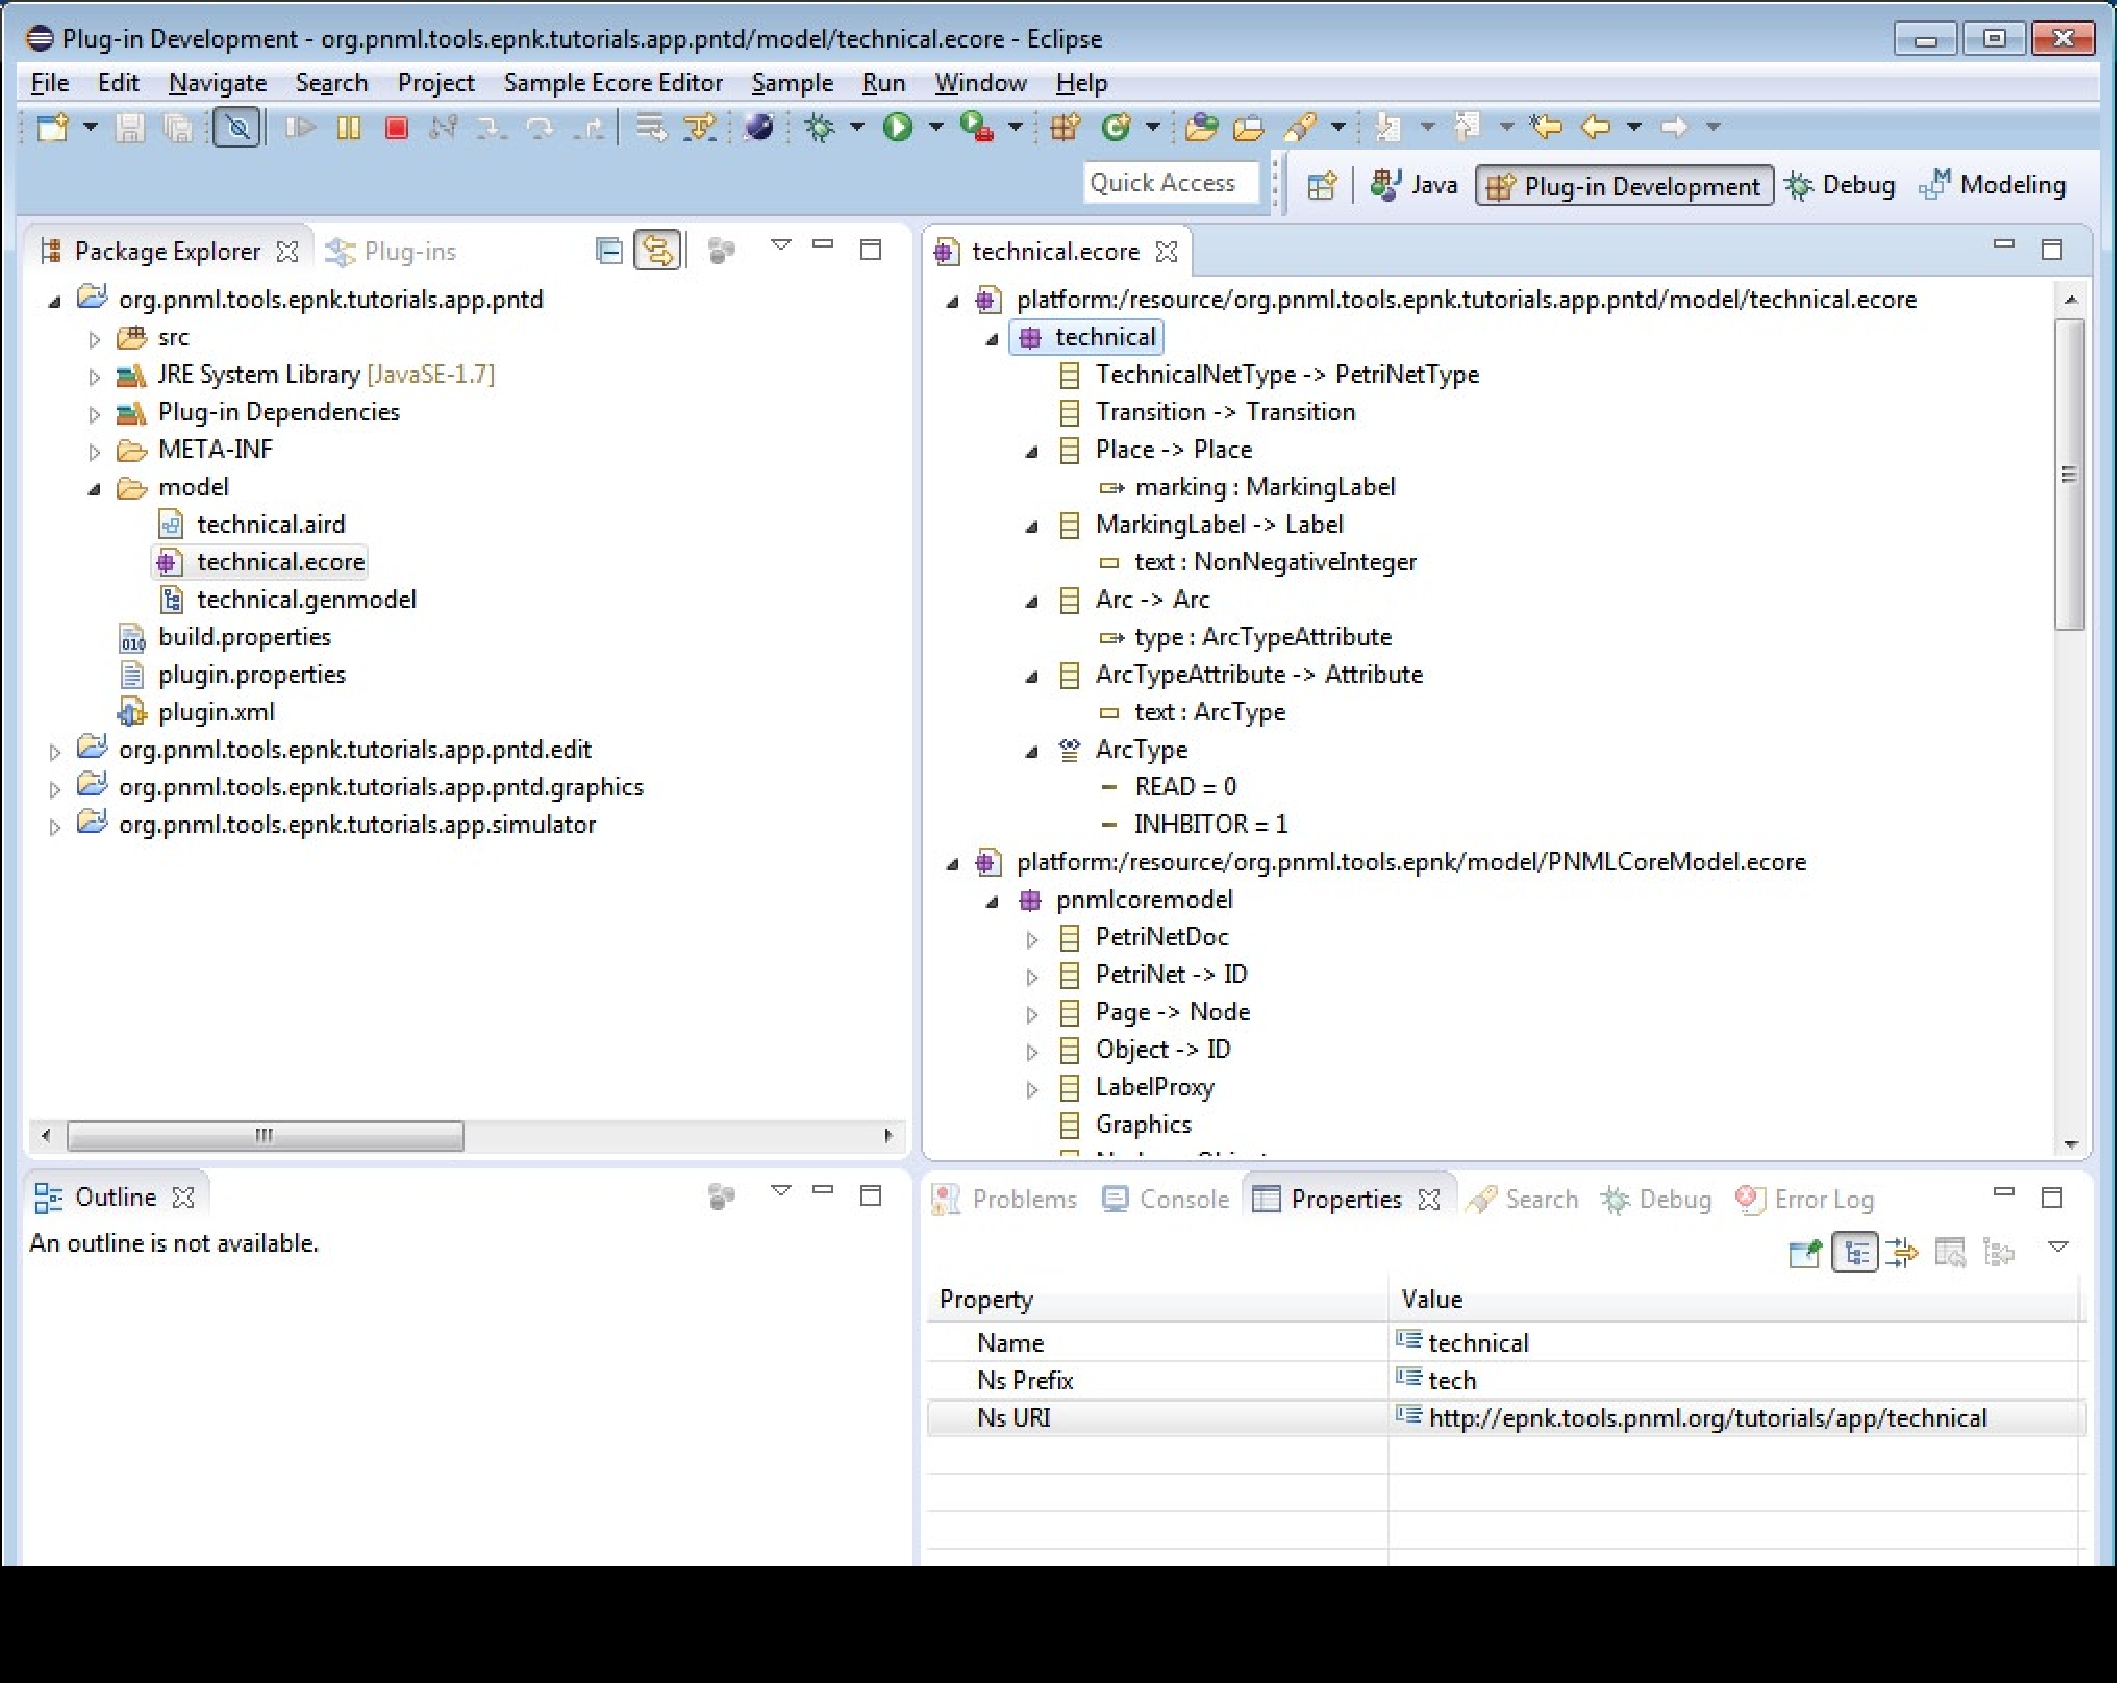
\includegraphics[scale=.34]{tutorial/ecore-tree-editor.pdf}}
  \centerline{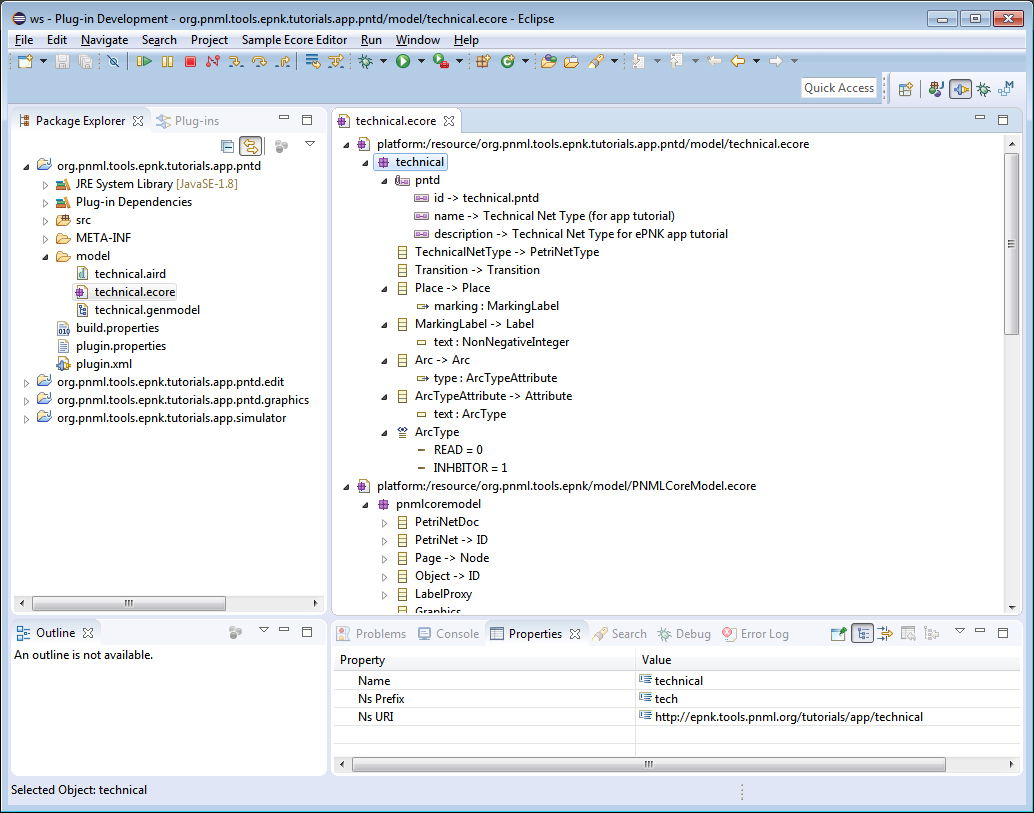
\includegraphics[scale=.34]{tutorial/ecore-tree-editor.jpg}}
  \caption{Ecore model of PNTD for technical net type in tree editor}
  \label{fig:tutorial:technical:pntd:ecore-tree}
\end{figure}

If you want, you can also open this model
in a graphical editor. To do this, you would need to switch to the ``Modeling''
perspective of your Eclipse workspace, and open the file {\tt technical.aird} by
double clicking on it; then navigate to ``Representation per category''
$\rightarrow$ ``Design'' $\rightarrow$ ``Entities'' $\rightarrow$ ``technical
class diagram'' and double click on $\rightarrow$ ``technical
class diagram''. Figure~\ref{fig:tutorial:technical:pntd:ecore-diagram} shows
the model when opened in the graphical editor.

\begin{figure}[hbtp!!]
  \centerline{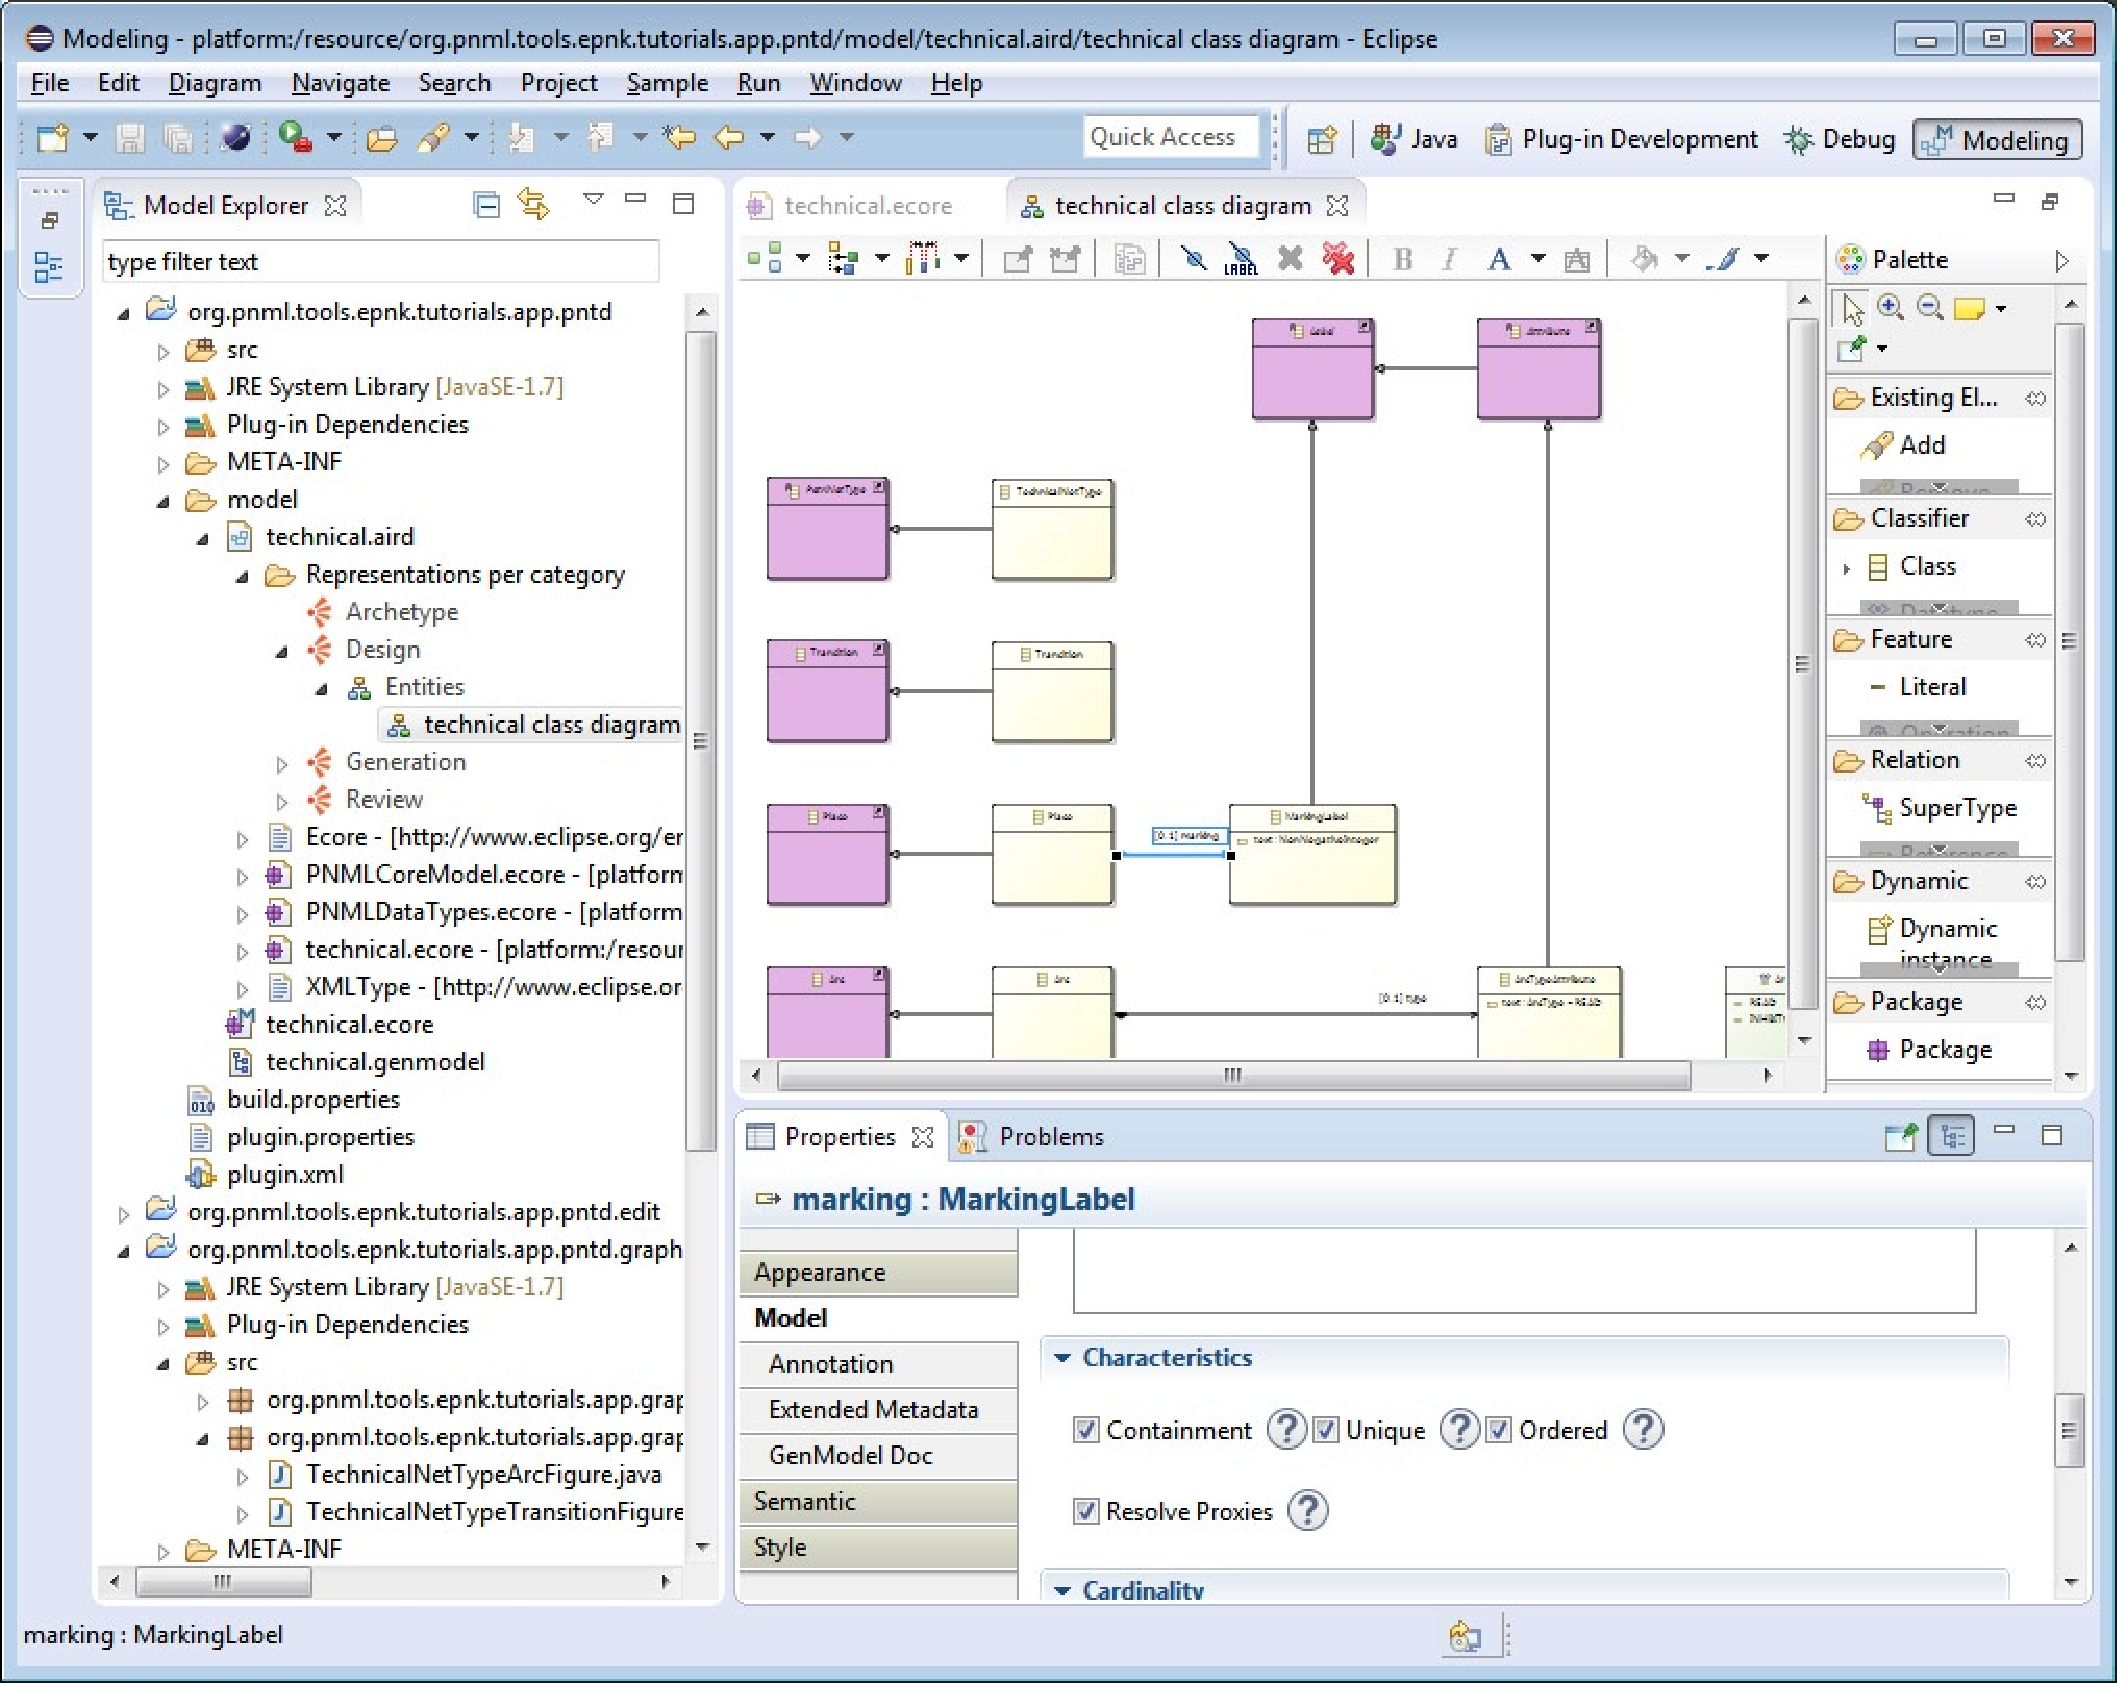
\includegraphics[scale=.34]{tutorial/ecore-diagram.pdf}}
  \caption{Ecore model for technical net type as diagram}
  \label{fig:tutorial:technical:pntd:ecore-diagram}
\end{figure}

We do not discuss the concepts of this model here again, since we
have discussed them already in Sect.~\ref{subsubsec:tutorial:concepts:pntd} in
Fig.~\ref{fig:tutorial:concepts:pntd}. 

\subsubsection{Creating the EMF project and model}
\label{subsec:tutorial:technical:pntd:ecore-creation}

Instead, we briefly discuss how to create such an EMF project and a model as
well as some technical details on how to edit some model features in this
subsection. Before you do this, it might be a good idea to switch back to
the ``Plug-in Development'' perspective in your Eclipse workspace.

A project which is based on a model from which code can be generated
automatically is called an \emph{EMF project}.  You can create a new empty
EMF project via the ``New'' action in the ``File'' menu of Eclipse. Select
``Other...'', and then, in the opened ``New'' dialog, select ``Empty EMF
project'' from category ``Eclipse Modeling Framework''.

In the newly created EMF project, you will find a folder {\tt model}, which is
where you should create a new Ecore model. A new Ecore model can be created
with the ``New'' action in the ``File'' menu. You will find the option ``Ecore
model'' in the ``Eclipse Modeling Framework'' category (try to use a
better name than ``My.ecore''); in the ``New'' dialog, you will be asked for
the top-level model object and the XML Encoding. The default should be
fine; make sure that the model object is set to {\tt EPackage}.

After you have created a new model, it will be shown in the Ecore tree
editor with a package with an empty name. Give a reasonable name to the package,
which uses non-capital letters, and choose a name space prefix and a unique URI
 representing your new package. The example from
Fig.~\ref{fig:tutorial:technical:pntd:ecore-tree} might give you an idea
on what to choose. Note however, that the domain
\url{http:\\epnk.tools.pnml.org} is reserved for the ePNK itself and for using
sub-domains of \url{tools.pnml.org} you would need to ask permission from
\url{http:\\www.pnml.org}.

In the newly created package, you should add one class which represents the
newly defined Petri net type. You can do that by right-clicking on the package
and then selecting ``New Child'' $\rightarrow$ ``EClass'' and give it a
reasonable name -- it is called {\tt TechnicalNetType} in our example. This
class must extend the class {\tt PetriNetType} from the {\tt pnmlcoremodel}. To this
end, you would need to set the class's ``ESuper Types'' in the properties view.
Before you can chose a class from the \emph{PNMLCoreModel}, you need to make
this package know to the editor. To do this, you need to load the resource containing
the {\tt pnmlcoremodel} in the tree editor. You can do this by right-clicking
somewhere in the tree editor and selecting ``Load Resource...''; then, in the
``Load Resource'' dialog, select ``Browse Target Platform Packages...'' and
select \url{http://org.pnml.tools/epnk/pnmlcoremodel}. Once you have done that,
you can select {\tt PetriNetType} as the ``ESuper Types'' in the properties view for your new class
for your Petri net type. Make sure to save this file right away.

Now you can continue adding the concepts of your new Petri net type. You should
add a class for each Petri net concepts that you want to extend and make sure
that it inherits from the corresponding class of the {\tt pnmlcoremodel}. The name
of these classes can, in principle, be any legal class name. But, you save a lot
of programming, if the class names are the same as in the  {\tt pnmlcoremodel} --
don't worry, since you have created them in a new package, there will be no
confusion with names, since your new classes live in a different name space. All new features
of your net type are represented by compositions to other classes, which need
to inherit from either {\tt Label} or {\tt Attribute} of the {\tt
pnmlcoremodel}. And these classes must have an attribute with name {\tt text}
and some data type. The data type can either be an existing data type, which
is built in to Ecore or defined in the ePNK, or a datatype defined in the new
package. In our example, the datatype {\tt ArcType} is an enumeration defined
in the package itself, the datatype  {\tt NonNegativeInteger} is defined by the
ePNK.

Note that in our example, the cardinality from the Petri net objects to its
features is $[0..1]$, which means that there can be zero or one of each feature
for every object of the respective type. But, the cardinality could also be $[0..*]$
allowing arbitrarily many instances of this feature for a single element. In the
tree editor for Ecore models, the value $-1$ as upper bound represents
``arbitrarily many''.

Note also that the reference from the Petri net object to its feature must
be compositions. In the Ecore model, this means that the property {\tt Containment}
of the respective reference must be set to {\tt true}.\\

At some point, it might be easier to edit and extend the Ecore model by using
a graphical editor. To this end, you can create a diagram for an existing Ecore
model: right-click on the file of the Ecore model and select ``Initialize Ecore
Diagram ...''; then, in the ``Create Representation File'' dialog, select a file
name and a folder for the diagram file (it should typically be in the same
folder as the model). In the ``Create Representation Wizard'', which opens after
a while, select ``Entities'' in category ``Design'' and continue; in the
next dialog select your package and give the diagram some name. In the diagram
editor that opens, double-click on ``here'' to create an initial representation
of you model. If you want to see related elements from other packages in this
diagram you can right-click on the diagram and select ``Add Related Elements''.
You will probably need to arrange the elements in a nicer way. In the end, don't
forget to save the diagram. Note that for opening the diagram again, you will
need to switch to the ``Modeling'' perspective of your Eclipse workspace as
discussed at the end of Sect.~\ref{subsec:tutorial:technical:pntd:ecore} for
Fig.~\ref{fig:tutorial:technical:pntd:ecore-diagram} already.

\subsubsection{Code generation}
\label{subsec:tutorial:technical:pntd:code-gen}

In order to plug in the PNTD defined by the Ecore model to the ePNK, we need to
first generate code from this model and make some adjustments to the code. The code will be generated
from a so-called \emph{gen model} that is associated with the Ecore mode and
defines some additional information for the code generator on how the code
should be generated and where the generated code should go.

In our example, the \emph{gen model} is the file {\tt technical.genmodel}. Once
opened in the \emph{EMF Generator} model editor, you can generate the code by
right-clicking on the top-level element and selecting ``Generate Model Code''
and ``Generated Edit Code''. You can also generate the other code, but you do
not need the ``Test Code'' and the ``Editor Code'' when using the model as
a PNTD for the ePNK.

When you have created a new EMF project and a new Ecore model, however, there
is no gen model yet. You first need to create the gen model for your new model
file.
You can do this by right-clicking on the file with the Ecore model and, then, selecting
``New'' $\rightarrow$ ``Other...'' and chosing ``EMF Generator Model'' from
category ``Eclipse Modeling Framework'' and following through the dialog. When
asked for the folder, make sure the gen model is in the same folder as the
model; when asked for the model URI, you will need to click on ``Load''\footnote
  {If clicking on load results in an error, there is probably some error in you
  Ecore model. Try to validate the Ecore model first and fix the error.}
and continue. At some point, a dialog for selecting the packages for which the
gen model should be generated will show up, which looks like the one
shown in Fig.~\ref{fig:tutorial:technical:pntd:gen-model-select-package1}.
Note that it crucial, that in this dialog you only select your package as
``Root package''; all the other ones, you should select in ``Referenced
generator models''. Before you continue, your selection in this dialog
should look like shown in
Fig.~\ref{fig:tutorial:technical:pntd:gen-model-select-package2}. Once you made
these selections, you can ``Finish'' the generation of the gen model.

\begin{figure}[hbtp!!]
  \centerline{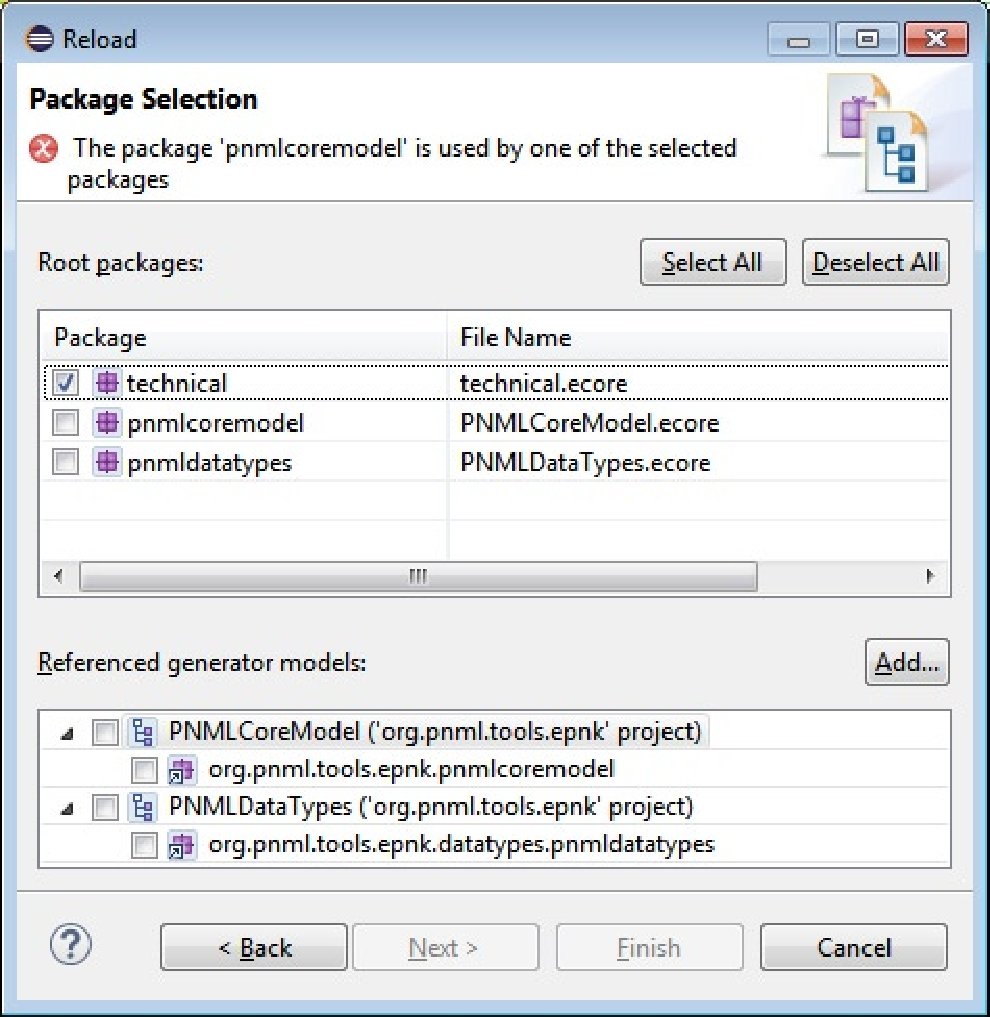
\includegraphics[scale=.48]{tutorial/PackageSelection.pdf}}
  \caption{Select Package Dialog}
  \label{fig:tutorial:technical:pntd:gen-model-select-package1}
\end{figure}

\begin{figure}[hbtp!!]
  \centerline{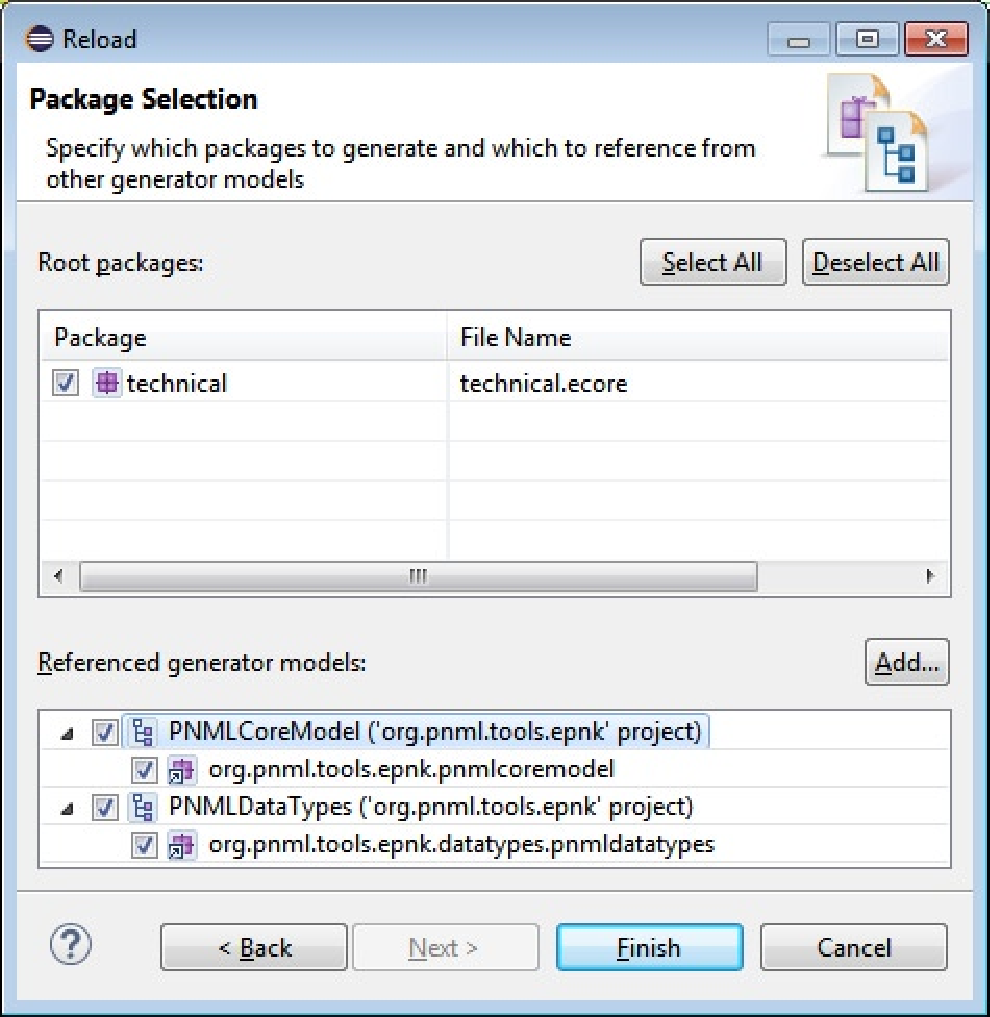
\includegraphics[scale=.48]{tutorial/PackageSelection2.pdf}}
  \caption{Select Package Dialog}
  \label{fig:tutorial:technical:pntd:gen-model-select-package2}
\end{figure}

Then the gen model for your model file should be created, and it should be open
in the ``Gen Model'' editor. Before you generate code from this new gen model,
you need to make two manual changes in this gen model. First, select the
top-most element and change one property in the properties view: change the property
{\tt Operation Reflection} in the category {\tt Model} to {\tt false}. Second,
open the top-level element and select the package element. For this package,
set the property {\tt Base Package} to some reasonable Java package name;
in our example, it is set to
{\tt org\qnsep{}pnml\qnsep{}tools\qnsep{}epnk\qnsep{}tutorials\qnsep{}app};
this setting directs the generator to generate the code in a
subpackage of this Java package.

Now, you can generate the model and the edit code from this gen model as
discussed above. The generated code should show no errors; if it does, you
probably forgot to change the property {\tt Operation Reflection} to {\tt
false} in the gen model after generating it.

Note that, if you should make changes in the model later on, you would need
to ``Reload'' your gen model again, so that it can become aware of the model
changes and update accordingly (reusing as much as possible from the existing
settings). In order to do that, first make sure that you have saved and closed
your model file. Then, right-click on the gen model and select ``Reload'' and
follow through the dialog which very much works like the dialog for
initially creating the gen model.

\subsubsection{Manual changes in the code}
\label{subsec:tutorial:technical:pntd:code-manual}

Before plugging in the generated net class to the ePNK, we need to make
two manual changes in the Java class generated for the class {\tt
TechnicalNetType}, which represents the new Petri net type defined in this
tutorial. In our example, this class can be found in the {\tt src} folder in
package {\tt
org\qnsep{}pnml\qnsep{}tools\qnsep{}epnk\qnsep{}tutorials\qnsep{}app\qnsep{}technical\qnsep{}impl}
and is called {\tt TechnicalNetType\optsep{}Impl}.

The two changes that need to be made in this class are the following: first,
the constructor of this class must be made public, which is necessary so that
the ePNK will be able to create new instances of this class. Second, the
{\tt toString()} method of this class must be implemented; it should return a
URI, which uniquely identifies Petri nets of this type in PNML. It must be
a string representing a URI. In principle, it can be any URI, you just need to
make sure that it is unique.

\begin{figure}[htbp!]
% \lstinputlisting[label=lst:tutorial:technical:pntd:code-manual,language=Java,tabsize=2,stringstyle=\small,%
\lstinputlisting[label=lst:tutorial:technical:pntd:code-manual,tabsize=2,stringstyle=\small,%
caption={Manual changes in class {\tt TechnicalNetTypeImpl}}]%
  {code/tutorial/TechnicalNetType-java.txt}
\end{figure}

Listing~\ref{lst:tutorial:technical:pntd:code-manual} shows the class
{\tt TechnicalNetTypeImpl}  with the changes made in lines 15--19 and 26--37,
highlighted in red. Note that for readability reasons, we have omitted some
comments, but otherwise the class is completely shown. In addition to
making the constructor public and implementing the {\tt toString()} method,
the changes are marked with the tag {\tt \@generated NOT}, which indicates
that there are manual changes to the generated code, and this way prevents the
manual changes being overwritten the next time the code is generated again
from the gen model.\\

The above changes are the only code that needs to be written manually for making
the new Petri net type work with the ePNK. In our example, we have three
additional Java classes, which are written completely manually. One implements
a Java constraint, which is discussed in
Sect.~\ref{subsec:tutorial:technical:constraints}. The other two are convenience
classes, which make it easier to implement our simulator and constraints later.
Since it is good practice and increases maintainability to have such convenience
classes with static methods, we briefly discuss them here, even though we do not
need them right away.

\begin{figure}[htbp!]
\lstinputlisting[label=lst:tutorial:technical:pntd:code-type,language=OCL,tabsize=2,stringstyle=\small,%
caption={Enumeration with all {\tt ArcType}s}]%
  {code/tutorial/ArcType-java.txt}
\end{figure}

In Listing~\ref{lst:tutorial:technical:pntd:code-type}, you can see a Java
enumeration for arc types. Remember, that our model of the PNTD has a similar
type; but in the model, there have been two possible values only: {\tt READ} and
{\tt INHIBITOR}. The end-user will only be able to set the type attribute
of arcs to these two values -- and the value can be left undefined. In
Listing~\ref{lst:tutorial:technical:pntd:code-type}, the enumeration defines
the values of all possible \emph{interpretations} of arc types. The static
method {\tt getArcType()} shown in Listing~\ref{lst:tutorial:technical:pntd:code-helper}
shows, how to compute the ``interpretation'' from the actual value set for
the arc and its source and target nodes it is connected to. It is crucial to
implement such an ``interpretation'' only once in the manually written code;
otherwise this code would be repeated and scattered all over the project
-- possibly even using different interpretations in different parts of the
software -- making maintenance a nightmare.

\begin{figure}[htbp!]
\lstinputlisting[label=lst:tutorial:technical:pntd:code-helper,language=OCL,tabsize=2,stringstyle=\small,%
caption={Class {\tt TechnicalNetTypeFunctions} with static helper methods}]%
  {code/tutorial/TechnicalNetTypeFunctions-java.txt}
\end{figure}

Note that the code from Listing~\ref{lst:tutorial:technical:pntd:code-type}
and~\ref{lst:tutorial:technical:pntd:code-helper} is written completely
manually, and does not run the risk of being overwritten by the code generator. Since the
code is part of an EMF project, where most code is automatically generated,
the code is tagged with {\tt \@generated NOT} anyway. This makes it
easy to search for all code which is not generated. In the project for the
PNTD, there are actually five manual changes: two of them in the class for the
net type and three manually written classes (the third class is discussed
later in Sect.~\ref{subsec:tutorial:technical:constraints}).

Since we might want to use the class {\tt TechnicalNetTypeFunctions} in our
other projects later, we need to export the Java package containing it
from this project. You can do that by using the ``Plug-in
manifest'' editor by double-clicking on the {\tt plugin.xml} and selecting
the ``Runtime'' tab. In that tab, you should add the respective Java package to
``Exported Packages'' by pressing the ``Add...'' button.

\subsubsection{Plugging in the PNTD}
\label{subsec:tutorial:technical:pntd:plugin}

The last step of defining a PNTD for the ePNK is actually plugging the generated
and manually changed class for the net type, {\tt TechnicalNetTypeImpl} in our
example, in to the ePNK. This could be done by using the Eclipse ``Plug-in
manifest'' editor. But, it is actually easier to do that directly by changing
the XML code of the {\tt plugin.xml}. To this end, open the {\tt plugin.xml}
file with the `Plug-in manifest'' editor by double-clicking on it and go to
the tab called ``plugin.xml''.

Listing~\ref{lst:tutorial:technical:pntd:plugin-xml} shows the snipped from the
{\tt plugin.xml}, which plugs the PNTD in to the ePNK. It is a usual Eclipse
\emph{extension}  referring to the \emph{extension point} {\tt
org.pnml.tools.epnk.pntd} (line~4), which is defined by the ePNK. The attributes
{\tt id} and {\tt name} is just a unique id and name for this new Petri net
type. The actual new type is defined in the {\tt type} element in lines 5--7;
its attribute {\tt class} refers to our class {\tt TechnicalNetTypeImpl},
which we had modified manually earlier and which defines the new Petri net type.
We need to refer to this class by its fully qualified Java class name
(including the packages); the description is just some text describing the new Petri net type.
 
\begin{figure}[htbp!]
\lstinputlisting[label=lst:tutorial:technical:pntd:plugin-xml,language=OCL,tabsize=2,stringstyle=\small,%
caption={{\tt plugin.xml} snipped plugging the PNTD in to the ePNK}]%
  {code/tutorial/plugin-xml-pntd.txt}
\end{figure}

Note that at this point, with only the project {\tt
org\qnsep{}pnml\qnsep{}tools\qnsep{}epnk\qnsep{}tutorials\qnsep{}app\qnsep{}pntd}
and the automatically generated project
{\tt org\qnsep{}pnml\qnsep{}tools\qnsep{}epnk\qnsep{}tutorials\qnsep{}app\qnsep{}pntd\qnsep{}edit},
we can use our Technical Petri
net type with the ePNK already. The only problem would be that \emph{read},
\emph{inhibitor} and \emph{reset} arcs would not be shown with a dedicated
graphics. All arcs would be graphically shown as \emph{normal} arcs. Moreover,
the end-user would still be able to draw arcs between arbitrary nodes, even
between pages. We discuss how to fix the latter problem in the next section, and
how to fix the first problem in Sect.~\ref{sec:tutorial:technical:graphics}.

Whenever you create a new Petri net type, it would be a good idea to check
whether your PNTD works with the ePNK at this point. Only after that, you should
proceed.

\subsection{Constraints}
\label{subsec:tutorial:technical:constraints}

In this section, we discuss how to define and plugin constraints for a
net type, so that the ePNK (and Eclipse in general) will take them into account.

As discussed in Sect.~\ref{subsubsec:tutorial:concepts:pntd}, we have two
constraints for our \emph{technical Petri net type}. The first is that an
arc should run from a place to a transition or the other way round, or it
should run from a page to a transition; moreover, only an arc running from 
a place to a transition can have a type (for the other arcs, the type attribute
should not be set). In Listing~\ref{lst:tutorial:concepts:pntd:ocl}, we have
already seen an OCL formulation of that constraint. The other constraint was
that there should be no duplicate read or inhibitor arcs between a place and
a transition. This constraint is realized as a Java constraint.

All constraints are defined in the our PNTD project {\tt
org\qnsep{}pnml\qnsep{}tools\qnsep{}epnk\qnsep{}tutorials\qnsep{}app\qnsep{}pntd},
which defined the PNTD. The reason
is that constraints conceptually are a part of a model. Actually, it would
be possible to include the constraints to the Ecore model. But, we follow
a slightly here.

\subsubsection{OCL constraint}
\label{subsubsec:tutorial:technical:constraints:ocl}

We start with discussing how to add the OCL constraint for properly connecting
arcs to the project. This can be done by pluging in an OCL constraint by
defining it in the {\tt plugin.xml} of the project
{\tt org\qnsep{}pnml\qnsep{}tools\qnsep{}epnk\qnsep{}tutorials\qnsep{}app\qnsep{}pntd}.
Listing~\ref{lst:tutorial:technical:constraint:ocl} shows the part of
{\tt plugin.xml} that defines a constraint provider, with the OCL
constrain for arcs. All of that snippet is necessary, but we highlight
some more important settings and features in the definition (marked in red).

The most important part is the actual OCL constraint, which we had shown
in Listing~\ref{lst:tutorial:concepts:pntd:ocl} on
page~\pageref{lst:tutorial:concepts:pntd:ocl} already. The OCL constraint
Listing~\ref{lst:tutorial:technical:constraint:ocl}
is shown as XML CDATA in order to escape all the special symbols of OCL in lines
30-39. Note, however that the first line from
Listing~\ref{lst:tutorial:concepts:pntd:ocl}, which gave the context is missing here.
This context is actually defined by the target element in lines 21--28:
the {\tt class} attribute defines the Ecore class it refers to by the name
{\tt Arc} of the class followed by the package URI of the model package in which
it is defined. The target also defines \emph{events} which cause the validator to check the
constraint again. In our example, these are set events of the features {\tt
source}, {\tt target} and {\tt type} of the arcs; this means that the validator
kicks is whenever one of these features is of an arc changes. This goes
together with the fact that we define the constraint as a \emph{live constraint}
(see line 10), which means that after any change an end-user makes (with respect
to the defined events), the constraint is checked. If the constraint should fail, the complete
action of the end-user will be undone. Therefore, the end-user cannot create
a model that is invalid with respect to a \emph{live constraint}, provided that
the event definition covers all features and events that might invalidate a
constraint of an arc. In our case, these features are {\tt source}, {\tt target}
and {\tt type}.

\begin{figure}[htbp!]
\lstinputlisting[label=lst:tutorial:technical:constraint:ocl,tabsize=2,stringstyle=\small,%
caption={{\tt plugin.xml} defining the OCL constraint for arcs}]%
  {code/tutorial/plugin-xml-ocl.txt}
\end{figure}

In addition, there is a \emph{severity} of the constraint (line~12), which is an
\emph{error} in our example, and \emph{language} of the constraint (line~9) is
defined as OCL. Moreover, there is a message, which will be output to the
end-user, whenever the validation fails -- and the message of the problem marker
attached to the model element.
The tag $\{0\}$ in this message, will be replaced with the object on which the
constraint failed (the \emph{target}).

Actually within the same constraint provider, more than one constraint can be
defined, which is indicated by the $\ldots$ in line~42. We will actually see an
additional constraint there when discussing the Java constraint in the following
section.\\

\begin{figure}[p!!]
  \centerline{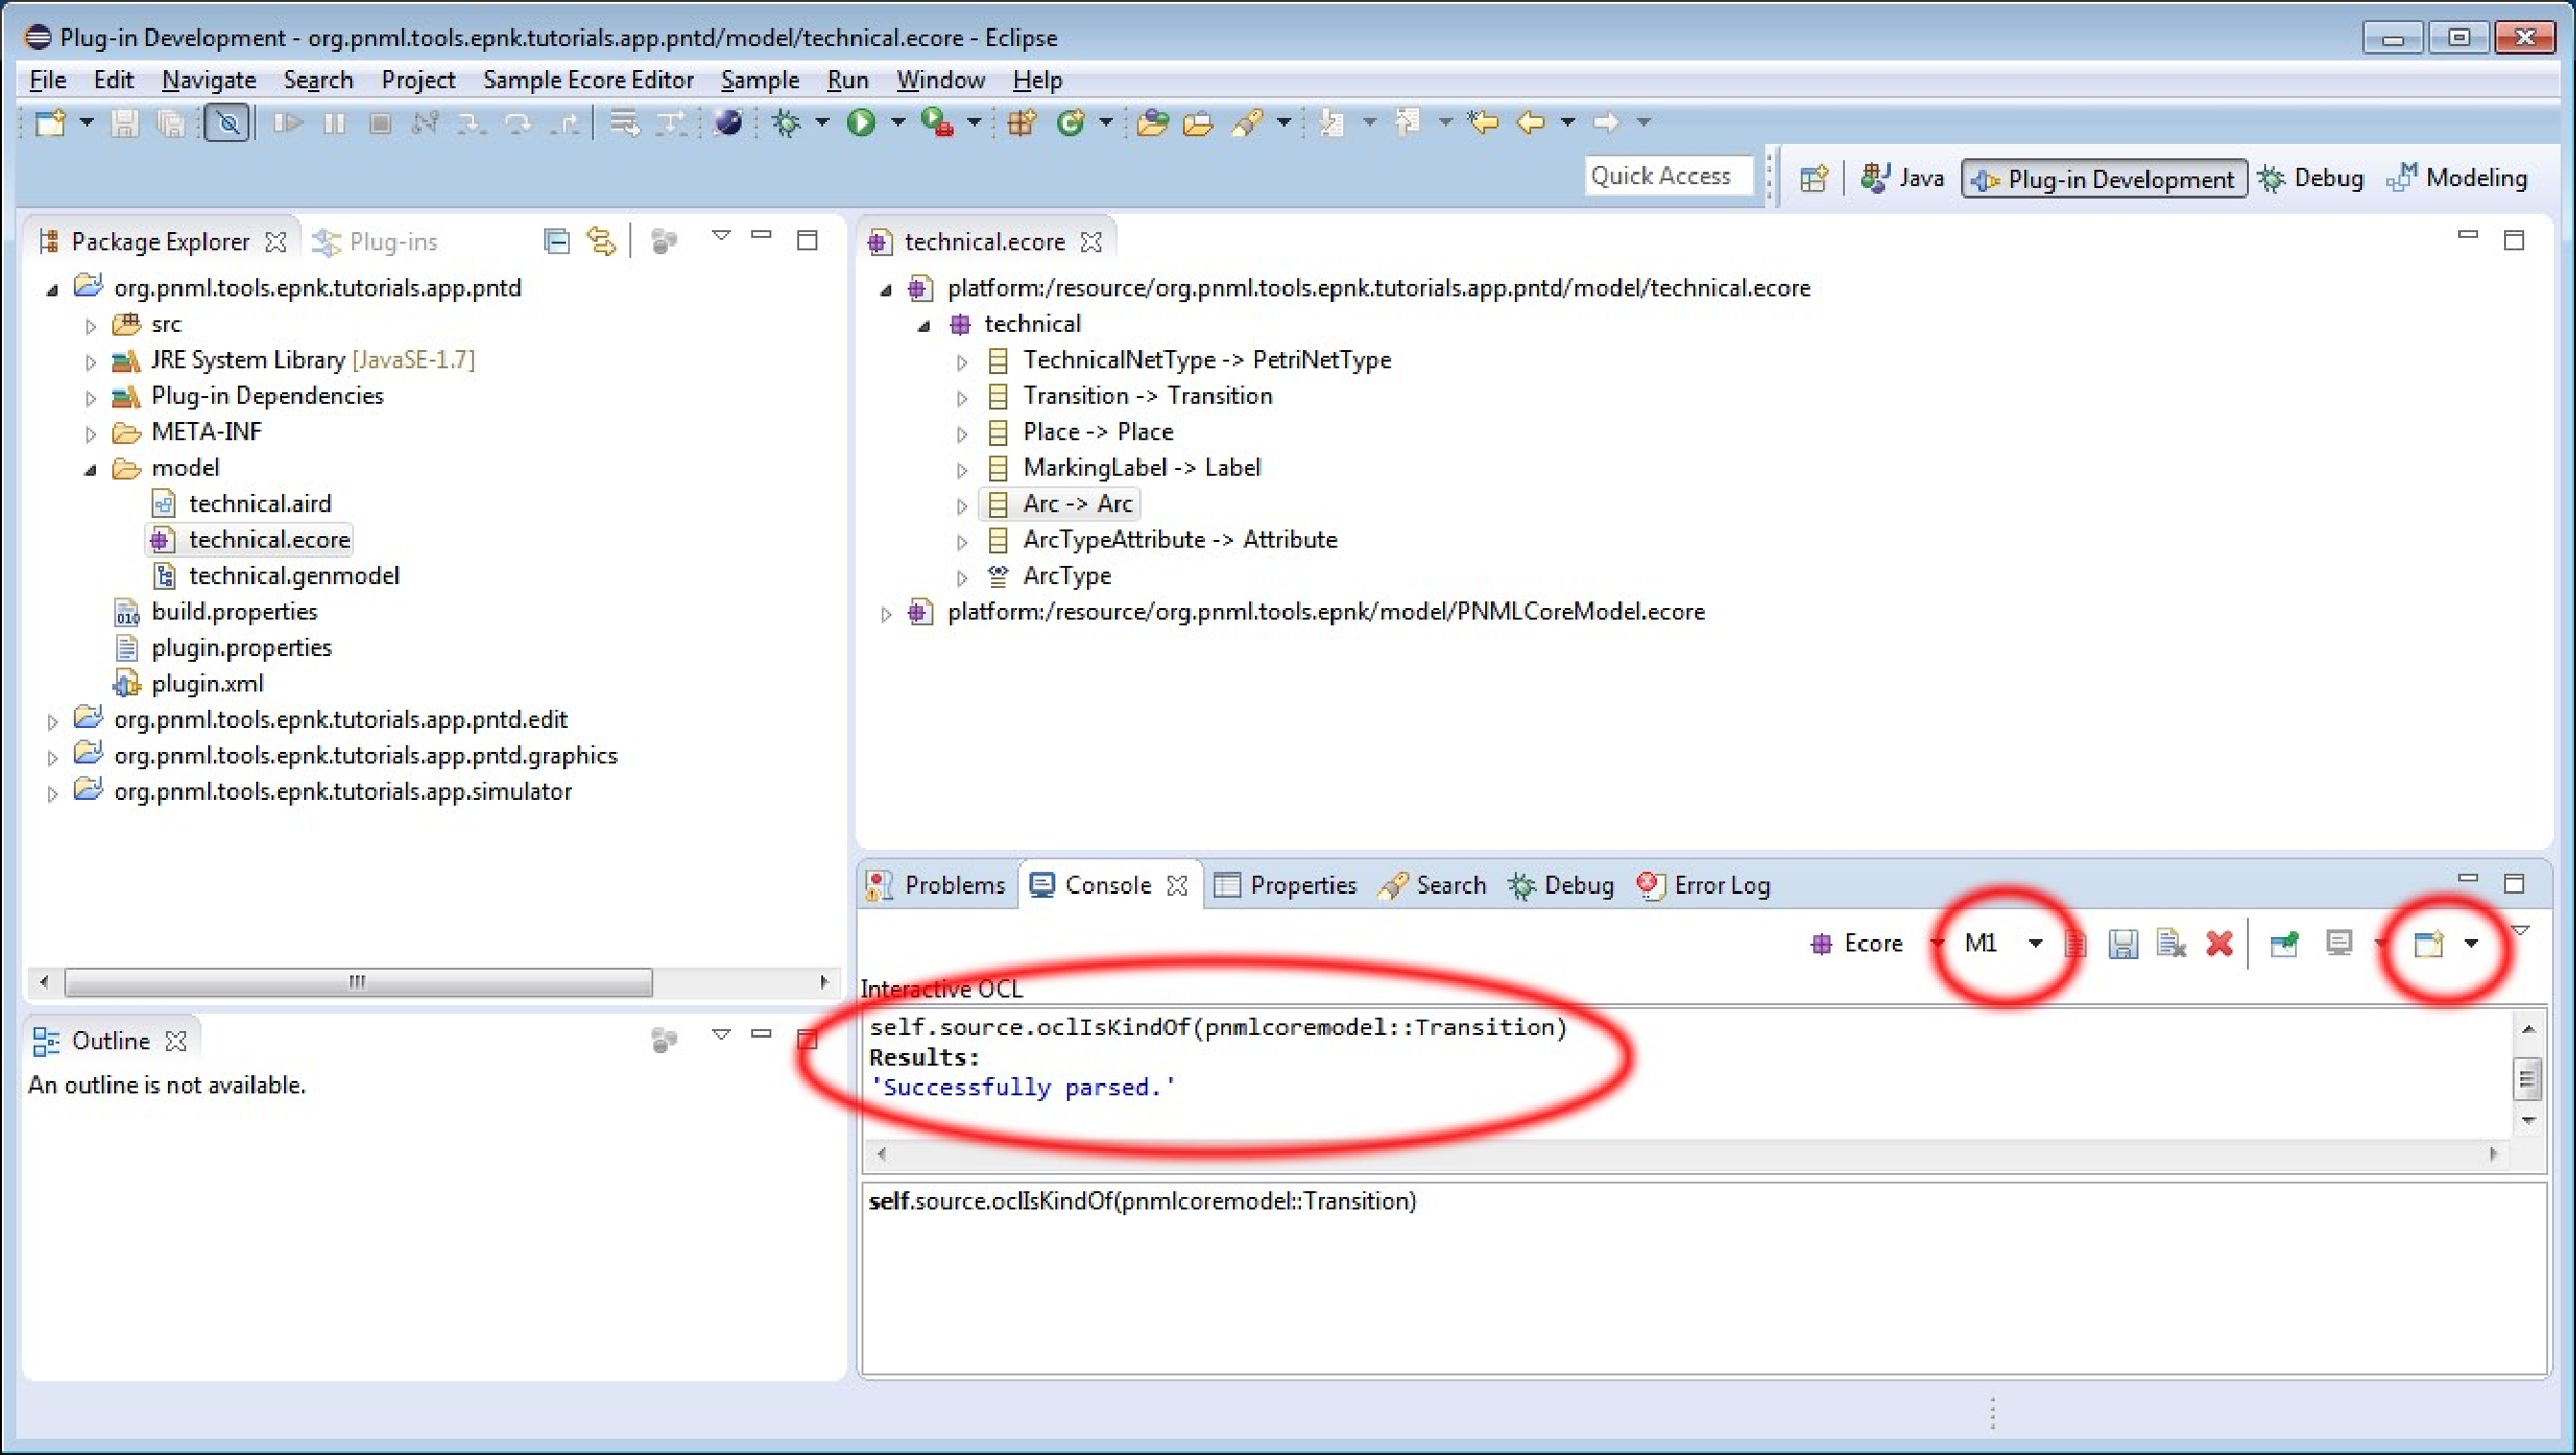
\includegraphics[scale=.27]{tutorial/ocl-console-m1.pdf}}
  \caption{OCL console in Eclipse development workbench}
  \label{fig:tutorial:technical:constraints:ocl:m1}
\end{figure}

Note that the OCL constraint must be syntactically correct, and getting the
syntax of OCL right might be a bit tricky if you do not have much experience.
Experimenting with the OCL syntax by changing the OCL constraint in the
{\tt plugin.xml}, starting the runtime workbench and testing whether the OCL
constraint works, and staring all over again, if it does not work, is way too
time consuming. We need a more efficient way to get the OCL syntax right --
and even a way to check how an OCL expression evaluates in a given situation.
To this end, we had recommended to install the ``OCL Examples
and Editors SDK'' feature to your Eclipse in
Sect.~\ref{sec:tutorial:technical:install:eclipse}. If this feature is installed
in Eclipse, you can open the ``Console'' view, and in that view select
``Interactive OCL'' as shown in
Figure~\ref{fig:tutorial:technical:constraints:ocl:m1}. In this console, select
M1 in the drop down menu (marked by a red circle). If you then select an element
in the Ecore editor, you can type some OCL constraint in the field at the bottom of the ``Interactive
OCL'' view and check whether it is syntactically correct (you even get some
syntax support, which indicates possible options while typing).
Once you type enter, the field on top will show whether the syntax of the OCL
constraint for the element selected in the Ecore model is syntactically correct.

Actually, the ``Interactive OCL'' console can not only be used for checking the
syntactical correctness of OCL constraints. If you start the runtime workbench,
and open an instance of a model, you can select an element of the instance, and
evaluate an OCL expression on this instance. For example, you could open a
PNML document and a page in the graphical editor, select an arc and evaluate the
constraint. This is shown in
Fig.~\ref{fig:tutorial:technical:constraints:ocl:m2}, where the OCL expression
{\tt self.type.text} is evaluated on an arc (the one running from place $p_7$
to transition $t_5$; the evaluation shows that it is an inhibitor arc. Note that
you need to switch the ``Interactive OCL'' console to ``Modeling level'' M2 for
this purpose.

\begin{figure}[p!!]
  \centerline{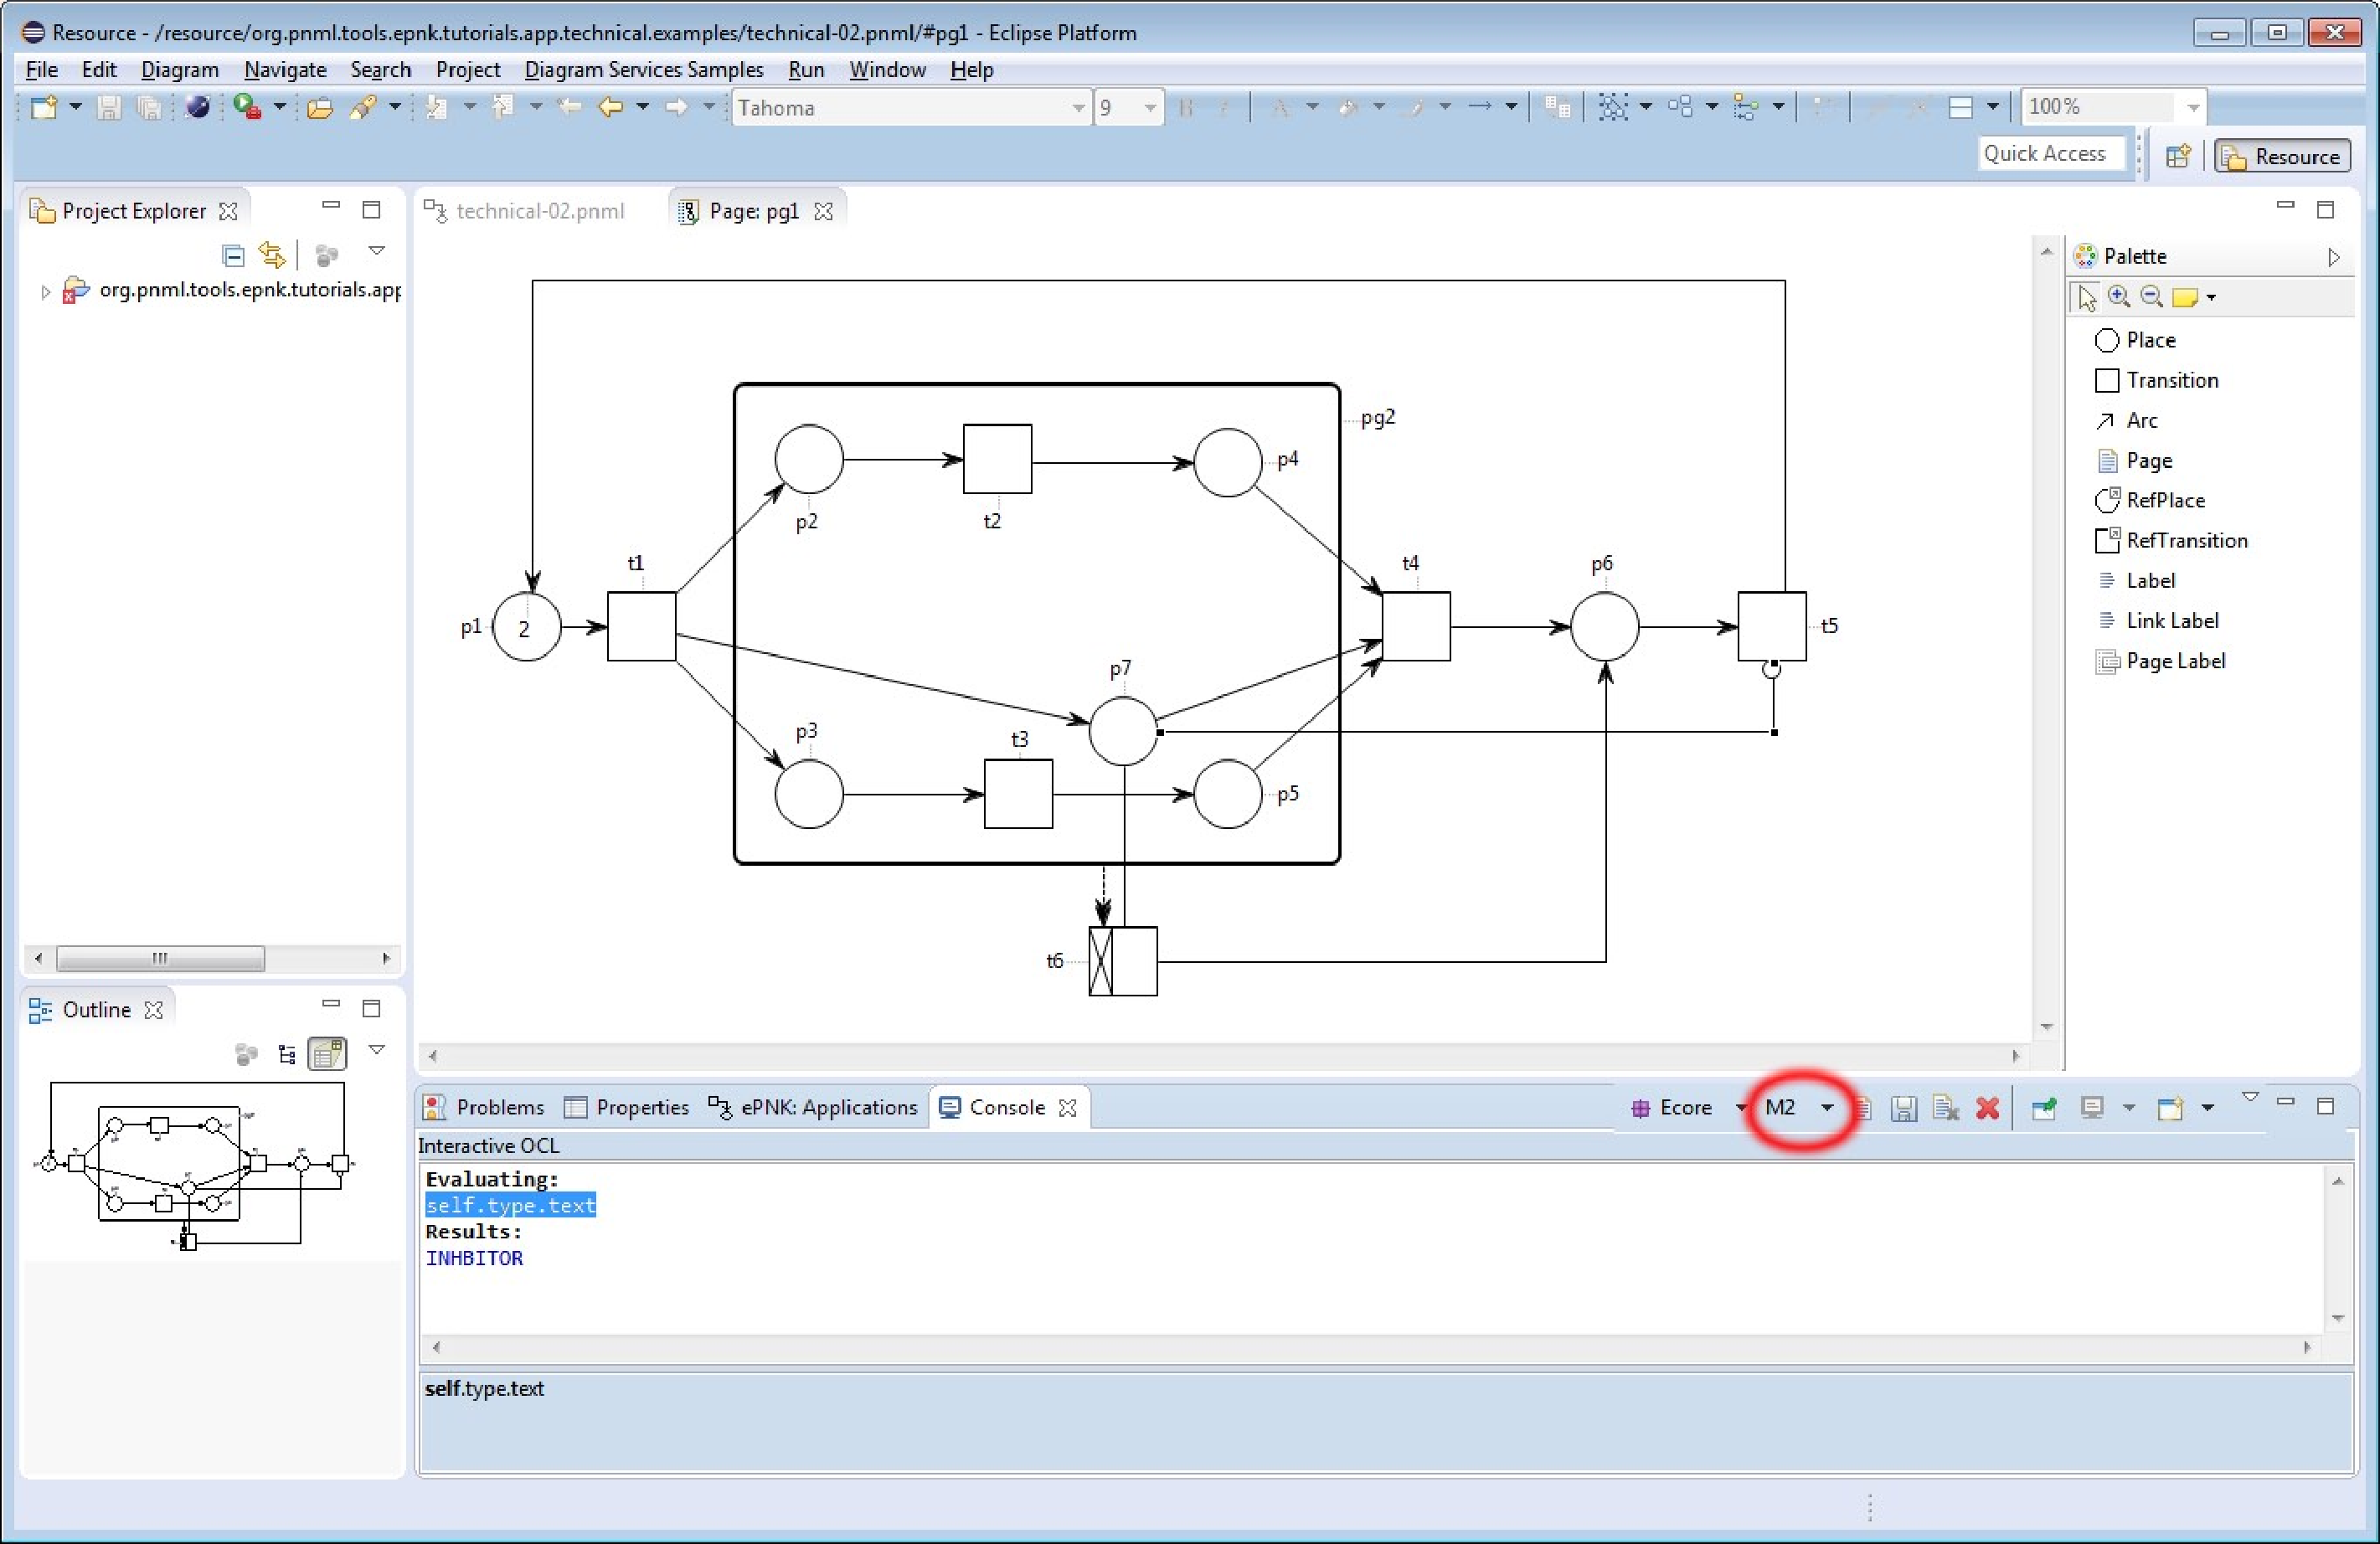
\includegraphics[scale=.27]{tutorial/ocl-console-m2.pdf}}
  \caption{OCL console in Eclipse runtime workbench}
  \label{fig:tutorial:technical:constraints:ocl:m2}
\end{figure}

Checking syntactical correctness, exploring the possible options for
expressions, and even for checking whether an OCL expression is evaluating as
expected, the ``Interactive OCL'' console is a very efficient tool.

\subsubsection{Java constraint}
\label{subsubsec:tutorial:technical:constraints:java}

Listing~\ref{lst:tutorial:technical:constraint:java} shows a Java implementation
of a constraint, which guarantees that there are no duplicate arcs of type
\emph{read} or \emph{inhibitor} between the same nodes. The {\tt validation()}
method of this class is called with some validation context from which the object on which the constraint
should be checked can be obtained (the \emph{target} that will be defined when
the constraint is plugged in). 

The implementation of the {\tt validation()} method first obtains the target
object form the validation context and checks whether it is an {\tt Arc} of
the our technical arc type. Then, it computes the ``interpreted'' type,
of the arc via the utility class {\tt TechnicalNetTypeFunctions}, which
we had discussed in Sect.~\ref{subsec:tutorial:technical:pntd:code-manual},
as well as the nodes to which the source and target of this arc resolve (in
case these are reference nodes); this is done with the {\tt NetFunctions}
utility class coming from the ePNK.

After that a so-called {\tt FlatAccess} object is obtained, which allows us to
obtain all arcs that conceptually belong to a node, even when the node is actually
split up via reference nodes on different pages. In case the arc is an
\emph{inhibitor} or \emph{read} arc, and it has a source node and if the
flatAccess object could be obtained, it iterates over all the other arcs that
have the source node as their source too. The set of all these arcs can be
easily obtained from the {\tt flatAccess} object. Than it checks for all
these {\tt other} arcs (if they are different from the arc itself), whether
the  {\tt other} arc is a duplicate, i.e.\ whether the other arc has the same
target and the same type. In that case, the {\tt validation()} method returns
a failure status using the context -- the singleton array contains the arc
on which the constraint had failed.

\begin{figure}[htbp!]
\lstinputlisting[label=lst:tutorial:technical:constraint:java,tabsize=2,stringstyle=\small,%
caption={Java class implementing the no duplicate arcs constraint}]%
  {code/tutorial/NoDuplicateArc-java.txt}
\end{figure}

Basically, a Java constraint is a class implementing a {\tt validation()}
method, which should return a failure status when the constraint is violated
on the target object and a success status otherwise. The rest is left to your
Java skills -- which, it in many cases, makes Java constraints easier to
formulate than OCL even tough the implementation looks a bit more verbose.

Note that the Java constraint is also marked {\tt @generated NOT} since it is
is manually written code in an plugin where most other code is automatically
generated. This is not strictly necessary since also this class is placed
in a Java package without any generated code. It is good practice to have 
clearly separate packages with generated code and manually written code.

After implementing a Java constraint it needs to be added to a constraint
provider, which is similar to plugging in OCL constraints. It is in this
part where it is defined on which target object the constraint should be
checked and whether it acts as a \emph{live constraint} or as  a \emph{batch
constraint}.
We chose to make the duplicate arcs constraint a \emph{batch constraint} only.
A \emph{batch constraint} is checked only when
the end-user explicitly starts a validation in the tree editor of a PNML
document.

Listing~\ref{lst:tutorial:technical:constraint:java} shows how the Java
constrain is added to our constraint provider from earlier (see
Listing~\ref{lst:tutorial:technical:constraint:ocl}, where some of the important
features are highlighted in red. But, except for the \emph{language}, which is
Java now, and the class attribute, which refers to the fully qualified name of
the Java class, this is very similar to the OCL constraint.
Note that since the constraint is a \emph{batch} constraint only, we do not need
to define an \emph{event} for the target object. The target itself refers to
the same Ecore class as before, the arc of our new model.

\begin{figure}[htbp!]
\lstinputlisting[label=lst:tutorial:technical:constraint:java-plugin,tabsize=2,stringstyle=\small,%
caption={{\tt plugin.xml} adding the Java constraint}]%
  {code/tutorial/plugin-xml-java.txt}
\end{figure}

\subsection{Graphical extensions}
\label{sec:tutorial:technical:graphics}

In this section, we discuss how to implement the graphical extensions for our
technical net type in more detail. As discussed in
Sect.~\ref{sec:tutorial:tool:nettype} and
Sect.~\ref{subsec:tutorial:concepts:graphics}, our technical net type needs a
customized graphical representation for arcs and for transitions.

In this tutorial, we demonstrate two different ways of implementing customized
graphics for some net object. The first one is on a high level of abstraction:
it, basically, changes attributes of the figure and composes the figure from other
figures. The second one is on a lower level of abstraction: it overrides the
method which draws the figure on the canvas. And, of course, both methods could
be combined. We had discussed this already in
Sect.~\ref{subsec:tutorial:concepts:graphics}.

In this section, we also discuss the mechanisms, which make sure that the
graphical representation is properly updated, when attributes that affect
the appearance change. Moreover, we discuss how to plug in the customized
figures into the ePNK. 

\subsubsection{Project set up}
\label{subsubsec:tutorial:technical:graphics:setup}

Since graphics is conceptually separate from the model defining the Petri net
type and since all code for graphics is programmed manually, the graphical
extensions are typically implemented in a separate project. This project is a normal
Eclipse \emph{Plug-in Project}. In our example, it is the project {\tt
org\qnsep{}pnml\qnsep{}tools\qnsep{}epnk\qnsep{}tutorials\qnsep{}app\qnsep{}pntd\qnsep{}graphics}.
But, the name ``pntd'' as part of the name indicates that this project belongs to the definition of the
Petri net type conceptually.

In case you need to create a new such project, you can simply create a new
\emph{Plug-in project} in your workspace by choosing ``New'' in the ``File''
menu and then selecting ``Plug-in project'' from category ``Plug-in
Development''; we recommend to switch to the ``Plug-in Development'' perspective
of Eclipse, which offers you the relevant tools and views for developing plug-ins in the toolbar and menus.

Once you have created a new plug-in project, you should add some dependencies
to this project, which you typically will need for graphical extensions for
a PNTD. You can do that by opening the ``Plug-in manifest'' editor by
double-clicking on the {\tt MNIFEST.MF} file in the {\tt META-MF} folder
and selecting the ``Dependencies'' tab. In addition to the project defining your
Petri net type, you should add the project {\tt org.eclipse.tools.epnk.diagram}
to the ``Required Plug-ins''.
In a plug-in project set up this way, you could then implement the classes
as discussed below yourself.

\subsubsection{Arc: composing a figure}
\label{subsubsec:tutorial:technical:graphics:arc}

We start with discussing the graphical extension for arcs, where we use
compose and configure the figure on a higher level of abstraction.
Listing~\ref{lst:tutorial:technical:graphics:arc} shows the class implementing
the graphical appearance of an arc of the technical net type. Part of this 
class, the {\tt setGraphics()} method, has been shown in
Listing~\ref{lst:tutorial:concepts:graphics:arc} an discussed in
Sect.~\ref{subsec:tutorial:concepts:graphics} already; therefore, we have
omitted this part indicated by ellipses and do not discuss this method here
again. Listing~\ref{lst:tutorial:technical:graphics:arc} shows the remaining
parts, in particular the constructor and the {\tt update()} method, which we
discuss below.
%
\begin{figure}[htbp!]
\lstinputlisting[label=lst:tutorial:technical:graphics:arc,tabsize=2,stringstyle=\small,%
caption={Class for arc graphics}]%
  {code/tutorial/arc-graphics-java-full.txt}
\end{figure}
%
We have discussed the {\tt setGraphics()} method (lines 28--30) already in 
Sect.~\ref{subsec:tutorial:concepts:graphics}. Based on the current type
(attribute {\tt arcType}) of the arc. This attribute is actually the type
that we had manually implemented (see
Sect.~\ref{subsec:tutorial:technical:pntd:code-manual}) in the PNTD project for
guaranteeing a uniform interpretation of the arc type values.
The initial value of this attribute is computed in the constructor (line~5) by using the
utility class {\tt TechnicalNetTypeFunctions}, which also was manually
implemented in the PNTD project. After setting this attribute the {\tt
setGraphics()} method is called from the constructor, in order to configure the
graphics accordingly.

Note that the figure class inherits from class {\tt ArcFigure}, which is defined
by the ePNK, along with similar classes for figures for transitions and places.
All these classes have an \emph{update()} method, which will be called whenever something that
might have an effect on the graphical appearance has changed. By default, a
change of the source, the target, and any of the arcs labels and attributes
defined in the respective net type are considered as potentially changing
the graphical appearance, triggering the ePNK to call the \emph{update()}
method of the respective {\tt ArcFigure}. It is up to the implementing figure
to react to this update by overriding the \emph{update()} method. In our
example, this method temporarily stores the latest type of the arc, and
then computes it again. If there was a change the {\tt setGraphics()} is
called again to properly configure the graphics.

Note that our implementation in lines 21-25 does slightly more. It
computes the target of the arc and issues a notification of some change
(not specified in detail) to the target. The reason for this is the following:
The graphical appearance of a transition depends on whether it has normal incoming
arcs or not. The transition figure will automtically be notified by the ePNK
when arcs are attached to it  or removed from it; but when the type of an
attached arc changes, the transition is not notified automatically by the
ePNK, because the type attribute belongs to the arc and not to the transition.
Therefore, the arc figure needs to notify the target transition about a
potential change, so that the transition figure can update its appearance
if necessary. 
Our implementation does that with the code in lines 21-25. Generally, the
implementation of the custom figures for a Petri net type can be mostly
independent of each other. But, if the appearance
of one element depends on features belonging to other elements, it would be
the responsibility of these other figures to issue a notification as
shown in 21-25. In our case, it is the {\tt target} of the arc taht needs to
be notified. Note that we do not need not notify the source of an arc, because
only for arcs pointing to a transition the end-user is allowed to change the
type (see discussion of constraints in
Sect.~\ref{subsubsec:tutorial:technical:constraints:ocl}). This shows that the
notification might take careful considerations, taking the appearances of
other figures and even constraints into account.

Issuing notifications actually needs some more consideration in order not to
issue cyclic notifications. This is the most important reason to
issue a notification only, if the type of the arc really changed. Another reason is
efficiency -- you do not need to redraw a figure if its appearance does not
change.

\subsubsection{Transition: drawing a figure}
\label{subsubsec:tutorial:technical:graphics:transition}

Listing~\ref{lst:tutorial:technical:graphics:transition} shows the complete
implementation the appearance of transitions.
It extends the {\tt TransitionFigure}, which is provided by the ePNK.
%
\begin{figure}[htbp!]
\lstinputlisting[label=lst:tutorial:technical:graphics:transition,tabsize=2,stringstyle=\small,%
caption={Class for transition graphics}]%
  {code/tutorial/transition-graphics-java-full.txt}
\end{figure}
%
Similar to arcs, the constructor computes whether, initially the transition has
normal input arcs and normal output arcs. The {\tt
TechnicalNetType\optsep{}Function} class provides two methods for that, which we
did not discuss though. The reason for implementing  these methods is again to make sure that there is a uniform
interpretation of transition having normal in and out arcs. In the {\tt update()} method, the old values of
both attributes are temporarily stored, then these attributes are recomputed.
If either of these values has changed the graphics is updated. Note however,
that this is not done by changing the figure as such. Instead the {\tt
repaint()} method is called, which is a method every figure has; it will
indirectly call the {\tt fillShape()} method, which implements how a transition
is drawn. We have seen this {\tt fillShape()} method in
Listing~\ref{lst:tutorial:concepts:graphics:transition} on
page~\pageref{lst:tutorial:concepts:graphics:transition} in
Sect.~\ref{subsec:tutorial:concepts:graphics} already.
Therefore, we do not discuss it here again. Note that the {\tt update()} method does not issue
notifications on other object since other objects' appearance does not depend on
features of a transition.

Note, however, that the graphical appearance of a transition might change
when an arc is added to a reference transition which refers to this transition.
But, the ePNK takes care of issuing an update, also when features of reference
transitions change. So, we do not need to do anything about that at all.


\subsubsection{Graphical extension}
\label{subsubsec:tutorial:technical:graphics:extension}

The different figures that define a graphical extension of a Petri net type need
to be combined and made available to the ePNK. This is done by
implementing a class, which extends the class {\tt GraphicalExtension} from the
ePNK. This class serves two purposes: first, it has methods with some meta
information on which Petri net types this class provides graphical
extensions for and saying for which elements of the Petri net it
provides graphical extensions; second, it serves as a factory that, for a given
net element, creates an instance of a figure implementing the graphical
representation of that element.

{\sloppy
Listing~\ref{lst:tutorial:technical:graphics:extension} shows
% the implementation of 
the class {\tt Technical\optsep{}Net\optsep{}Graphics}, which combines the
features of our graphical extensions and makes them available to the ePNK.
The method {\tt getExtendedNetTypes()} returns a list of classes representing
the Petri net types for which this is an extension. Note that, this list does
not refer to
Java classes but to classes from the Ecore models ({\tt EClass}) defining the
Petri net type. Programmatically, these classes are available via objects that
represent this package which have type {\tt EPackage}. An instance of this
class can be obtained from a class in the generated code; in our example,
it is the available via the generated interface {\tt TechnicalPackage}. The
call  {\tt
TechnicalPackage.eINSTANCE.get\optsep{}Technical\optsep{}Net\optsep{}Type()}
returns the Ecore class {\tt TechnicalNetType}. Note that we can obtain the
Ecore classes representing the place, the transition, and arc of the technical
package in a similar way. Basically, The implementation of method {\tt
getExtended\optsep{}Net\optsep{}Types()} says that it is responsible for Petri
nets of {\tt Technical\optsep{}Net\optsep{}Type}. Note that it is actually
possible that the same graphical extension provides graphical extensions for several 
Petri net types. This can be either by adding more net
types to the list returned by {\tt getExtendedNet\optsep{}Types()}; or this can
be by saying that the graphical extension applies to subtypes of the Petri net type,
which we briefly discuss later.
}

\begin{figure}[htbp!]
\lstinputlisting[label=lst:tutorial:technical:graphics:extension,tabsize=2,stringstyle=\small,%
caption={The graphical extension class for the Technical Net type}]%
  {code/tutorial/graphical-extension-java.txt}
\end{figure}

Similarly, for a given net type the method {\tt getExtendedNetObjects()} 
returns a list of Ecore classes extending places, transition and arcs, for which
it defines graphical extensions. At last, there are methods which for a given
net element provide a new instance of a figure for that element. In our case,
it returns the figures that we have defined in
Sect.~\ref{subsubsec:tutorial:technical:graphics:arc} for arcs and
Sect.~\ref{subsubsec:tutorial:technical:graphics:transition} for transitions,
provided that the arc or transition are of the respective Java type.\\

Note that the class {\tt GraphicalExtension} of the ePNK, has several other
methods, which allow us to define a priority for a graphical extension, which
might be needed when several extensions for the same net type and element would be
available. Moreover there are methods for defining whether the extension would
apply for all subtypes of a given net type and for extended elements. By
default, a graphical extension has priority $0$ and does neither apply to
subtypes of net types nor to extended elements. Changing these setting might
have quite far-reaching consequences, which we do ot discuss here in detail.
Therefore, we recommend not to change the defaults.

\subsubsection{Pluging in the graphical extension}
\label{subsubsec:tutorial:technical:graphics:plugin}

Ultimately, the {\tt GraphicalExtension} needs to be plugged in to the ePNK,
so that the ePNK will know about it. The easiest way to do that is
again to copy a XML snippet to the {\tt plugin.xml} of the project where the
graphical extension class is defined. A minor complication might be that
the {\tt plugin.xml} does not exist in a newly created plug-in project. So
we need to create it first. The easiest way to do that is opening the ``Plug-in
manifest'' as discussed above and to select the ``Extensions'' tab; 
pressing the ``Add...'' button, but cancelling the opened dialog right away.
After that, we have create a new and empty {\tt plugin.xml} file in our project.

The snippet that plugs in our {\tt TechnicalNetGraphics} to the ePNK is shown
in Listing~\ref{lst:tutorial:technical:graphics:plugin}. The parts which can
be freely chosen are marked in red: the {\tt id}, the {\tt name}, the {\tt
class} and the {\tt description}. The {\tt
class} attribute, must of course refer to a Java class extending {\tt
GraphicalExtension} by a fully qualified name of a Java class; and this class
must be on the class path of this project; a warning in the {\tt plugin.xml}
will indicate if this is not the case. The {\tt point} attribute of the
extension must refer to the ePNK extension
point {\tt org.pnml.tools.epnk.diagram.graphics} for graphical extensions.

\begin{figure}[htbp!]
\lstinputlisting[label=lst:tutorial:technical:graphics:plugin,tabsize=2,stringstyle=\small,%
caption={Snippet from {\tt plugin.xml} for pluggin in the graphical extension}]%
  {code/tutorial/graphical-extension-plugin.txt}
\end{figure}

Once you have finished a plugin project with a graphical extension, it is a good
idea to check whether it works in the ePNK. To this end, start the runtime
workbench of Eclipse and, in this runtime workbench create a net of your new type and
open a graphical editor on it.
If your graphical extensions do not properly appear, it is a good idea to
start the runtime workbench in a debugger. By setting a break point in the
constructor of the graphical extension, you can see whether your extension is
ever loaded by the ePNK. If not, you probably forgot to plug in the extension,
or the class the extension is referring to does not exist at all or is
not on the class path. If the class is loaded, you might set break point
in the other methods and see what happens when the ePNK calls these methods.

\subsection{Simulator application}
\label{subsec:tutorial:technical:application}

At last, we discuss the technical details of the implementation of the
simulator for our technical Petri net type. In our example projects, this
is realized in a separate EMF project: {\tt
org\qnsep{}pnml\qnsep{}tools\qnsep{}epnk\qnsep{}tutorials\qnsep{}app\qnsep{}simulator}.
It is realized as an EMF project, since we extend the \emph{ePNK
annotation model} by some specific types of annotations. This is done by an
Ecore model which extends the ePNK annotation model.

In the following, we briefly discuss our extended annotation model, which we
call {\tt technicalannotations} (refering to our \emph{technical} net type),
where the focus is on how to create it and how to generate code from it. Then,
we discuss some core parts of the implementation, a class representing a marking
of nets of our technical Petri net type, and core functions for realzing the
functionality.

In the end, we discuss the \emph{presentation handler} defining the graphical
representation of the annotations, the \emph{action handler} which handles user
actions, and how to combine all the parts into an application, and how to plug
in the simulator application to the ePNK.

\subsubsection{Annotation model}
\label{subsubsec:tutorial:technical:application:annotation}

We had discussed the annotations that we need for our simulator already in
Sect.~\ref{subsubsec:tutorial:concepts:app:annot}. The Ecore model of
these annotations was shown in Fig.~\ref{fig:tutorial:concepts:app:annot:model}
on page~\pageref{fig:tutorial:concepts:app:annot:model}.
Basically, there is an annotation for \emph{weakly enabled transitions}, which
has an attribute saying whether the transition is truly \emph{enabled} or only
weakly enabled. Moreover, there is an annotation for the arcs that prevent the
true enabledness of a transition; we call this annotation {\tt
InvolvedArc}. This annotation allows the end-user to activate or deactivate
these arcs, where the current status is indicated by attribute \emph{active}.
The {\tt InvolvedArc} is associated with the corresponding {\tt
EnabledTransition} annotation so that we can navigate back and forth between
these related annotations.
The {\tt EnabledTransition} is also used for annotating reference transitions
that refer to enabled transitions.
Conceptually, these {\tt EnabledTransition} annotations belong to each other,
which is represented by the reference {\tt ref} and {\tt resolve} which are
opposites of each other. At last, there is an annotation indicating the
{\tt Marking} of a place or an associated reference place. The attribute {\tt
value} represents the current number of tokens on that place.

When creating the project from scratch, you would first create an empty
\emph{EMF project} and then a new \emph{Ecore model} as discussed in
Sect.~\ref{subsec:tutorial:technical:pntd:ecore-creation}. Again, you would give
the package a reasonable name, {\tt techsimannotations} in our example, and
chose some \emph{namespace} prefix and a \emph{URI} for this package.

Then, you would create the classes of the model as shown in
Fig.~\ref{fig:tutorial:concepts:app:annot:model} on
page~\pageref{fig:tutorial:concepts:app:annot:model}. Note that these
classes inherit from the ePNK ;  the {\tt Marking}
inherits also from {\tt TextualAnnotation}. Both class {\tt
ObjectAnnotation} and {\tt TextualAnnotation} come from the ePNK base package
\url{ http://tools.pnml.org/epnk/netannotations/1.0}. Before you can add these
classes as super types to your classes, you must load the
\url{http://tools.pnml.org/epnk/netannotations/1.0} as a resource to your editor
by using the ``Load Resource'' action as discussed in
Sect.~\ref{subsec:tutorial:technical:pntd:ecore-creation}; make sure that you
use the ``Browse Target Platform Packages...'' feature to selec  the package 
\url{http://tools.pnml.org/epnk/netannotations/1.0}.

Then, you can choose the super types for your new annotation classes. Note that
in Ecore models, it is possible to chose more than one super type; Ecore
supports multiple inheritance.

In this Ecore model there occurs one feature which we have not
discussed before. There are references which are \emph{opposites} of each other,
in a sense they form two ends of the same association. In order to create such
opposite references in the Ecore model editor, you would create two independent
references in opposite directions first; then, you would make them
\emph{opposites} of each other:
to this end, you would chose one reference, and in the properties set the
property ``EOpposite'' choosing the reference into the other direction.

After that, you can create an EMF Generator model from your new Ecore model and
generated code from it as discussed in
Sect.~\ref{subsec:tutorial:technical:pntd:code-gen}. In the ``Package
Selection'' dialog when creating a new generator model, remember that the only
package selected in section ``Root package'' should be your new model; for all
models loaded from the ePNK, the gen models should be selected in the
``Referenced generator models''. Don't forget to set the {\tt Base Package}
property in your generator model and to set the {\tt Operation Reflection} to
{\tt false} as discussed in Sect.~\ref{subsec:tutorial:technical:pntd:code-gen}.

Once the gen model is created, you can generate the model code. Note that, for
the annotation model, it is enough that you generate the model code; you do not
need to generate the edit, the editor or the test code.

Once you have generated the code for your annotations, you can start realizing
the actual simulator application. Before you start with that, you might want to
add some additional dependencies to your project (by opening the  ``Plug-in
manifest'' editor clicking on the {\tt plugin.xml}). The code generator will
have added some dependencies to your project already.

In addition to the project which defines your PNTD, the project {\tt
org\qnsep{}pnml\qnsep{}tools\qnsep{}epnk\qnsep{}tutorials\qnsep{}app\qnsep{}pntd}
in our example, and the ones which the code generator has added already, you
will probably need to add the following projects to the dependencies of your
project:
{\tt org\qnsep{}pnml\qnsep{}tools\qnsep{}epnk\qnsep{}applications} and
{\tt org\qnsep{}eclipse\qnsep{}gmf\qnsep{}runtime\qnsep{}diagram\qnsep{}ui}.

\subsubsection{NetMarking}
\label{subsubsec:tutorial:technical:application:marking}

In a simulator, the \emph{marking} of a net plays a key role since it
represents the current state of a Petri net in a simulation. Conceptually, a marking is
a mapping from places to integers. So the marking could be represented as
a Java \lstinline|Map<Place,Integer>|. But, accessing a Java
\lstinline|Map<Place,Integer>| and keeping it consistent, might be a bit
tedious. Therefore, we implemented a class {\tt NetMarking} in our simulator,
which eases the access and update of such mappings. Internally, the marking is
represented as a Java \lstinline|Map<Place,Integer>|; but the class {\tt
NetMarking} provides some methods for easier manipulating the marking.

Programming this class is straight-forward; therefore, we do not discuss the
implementation here. You can look up the implementation of this class
in the project
{\tt
org\qnsep{}pnml\qnsep{}tools\qnsep{}epnk\qnsep{}tutorials\qnsep{}app\qnsep{}simulator}
of the code provided for this tutorial; you will find it in the Java package 
{\tt
org\qnsep{}pnml\qnsep{}tools\qnsep{}epnk\qnsep{}tutorials\qnsep{}app\qnsep{}simulator\qnsep{}marking}.
Here, we show the available methods of this class only, since we will use them
later in the implementation of the simulator.
Listing~\ref{lst:tutorial:technical:application:marking} shows all the methods
of class {\tt NetMarking}.

\begin{figure}[htbp!]
\lstinputlisting[label=lst:tutorial:technical:application:marking,tabsize=2,stringstyle=\small,%
caption={Methods of the class {\tt NetMarking}}]%
  {code/tutorial/netmarking-java.txt}
\end{figure}

\subsubsection{Core functions}
\label{subsubsec:tutorial:technical:application:corefunctions}

In this section, we discuss the implementation of the method which computes from
a given marking and a given enabled transition a new marking, which results from
firing this transition. This methods implements the core
functionality of our simulator.

In order to make it easy to implement this method, our
simulator implements some more basic functions. The first two methods compute
for a given marking how many tokens a transition will consume from each place
and how many tokens it will produce on each place. Actually, the number of
consumed and produced tokens for each place can be considered to be markings
again. So the result type of these methods is {\tt NetMarking}. The
implementation of these two methods are shown in
Listing~\ref{lst:tutorial:technical:application:produce-consume}.
The implementation is straight-forward: Initially an new empty marking is
created. Then, the methods iterate over all in-coming or out-going
arcs, and, for each normal arc, incrementing the marking for the source
or the target place, respectively. In the end, the resulting marking is
returned.
The only interesting point is that we, again, use the {\tt FlatAccess} for
obtaining all in-coming and out-going arcs of the transition and for resolving reference
places to the actual place they refer to. As we see later, our simulator
has a method, which obtains an instance of {\tt FlatAccess} for the net on
which the application is running, and we use this method {\tt getFlatAccess()}
in these methods {\tt consumes} and  {\tt produces}.

\begin{figure}[htbp!]
\lstinputlisting[label=lst:tutorial:technical:application:produce-consume,tabsize=2,stringstyle=\small,%
caption={Implementation of the {\tt consumes()} and {\tt produces()} methods}]%
  {code/tutorial/produce-consume-java.txt}
\end{figure} 

There are two other functions, which we need in our simulator: {\tt
isWeakly\optsep{}Enabled()}, which computes for a given marking whether a given
transition is weakly enabled, meaning that considering normal arcs only, the transition
would be enabled; the other {\tt preventingArcs()} computes for a given marking
and a given weakly enabled transition, which \emph{read} arcs and which
\emph{inhibitor} arcs would prevent it from firing anyway. The implementation
of both of these methods is shown in
Listing~\ref{lst:tutorial:technical:application:weakly-enabled}. Note that due
to our {\tt consumes()} method and the {\tt isGreaterOrEqual()} method for
markings the implementation of the {\tt isWeaklyEnabled()} method is very
simple. We just need to compute that consumed tokens of the transition and
check whether the marking is greater than that. For computing the preventing
arcs, we need to iterate over all the incoming \emph{arcs}: a \emph{read arc}
will be added to the result, if its source place does not have a token in the
given marking; a \emph{inhibitor arc} will be added, if the source place has a
token in the given marking.

\begin{figure}[htbp!]
\lstinputlisting[label=lst:tutorial:technical:application:weakly-enabled,tabsize=2,stringstyle=\small,%
caption={Code for {\tt isWeaklyEnabled()} and {\tt preventingArcs()}}]%
  {code/tutorial/weaklyEnabled-java.txt}
\end{figure} 

At last, it is easy to implement the {\tt fireTransition()} method based on the
previous methods.  Listing~\ref{lst:tutorial:technical:application:fire} shows
the implementation of this method. It starts with copying the marking from
which the transition should be fired. Then, it consumes the token from the
incoming normal arcs, resets the places on pages that have a reset arc to
the transition; and, at last, it produces the tokens on the out-going normal
arcs.
The trickiest part is the reset of all places on sub pages, even though the
implementation is straight-forward.

\begin{figure}[htbp!]
\lstinputlisting[label=lst:tutorial:technical:application:fire,tabsize=2,stringstyle=\small,%
caption={Impementation of the {\tt fireTransition()} method}]%
  {code/tutorial/fire-java.txt}
\end{figure}

\subsubsection{Annotation functions}
\label{subsubsec:tutorial:technical:application:annotationfunctions}

In Sect.~\ref{subsubsec:tutorial:technical:application:corefunctions}, we have
discussed the methods which implement pure functionality on Petri nets. In order
to visualize the markings, we need some additional functions or methods which
ultimately show the markings in a net. To this end, we need to convert a
marking into a net annotation. And we need a way to convert a net annotation
into a marking. This separation would actually not be strictly necessary, but it
makes the design clearer and the easier implementation easier  understand.

Basically, we need the following methods: One for computing the initial marking
from the net itself, one for computing a marking from the current annotation of the net,
and one for creating a new net annotation from a given marking (showing the
marking as well as the weakly enabled transitions and the involved arcs).

Listing~\ref{lst:tutorial:technical:application:compute-initial} shows the
method for computing the initial marking of a net. The method
initializes a new empty marking. Then, it iterates over all the places of
the net (using the {\tt FlatAccess} object from the application again) and sets
the value of the marking for each place (if it is not zero) accordingly.

\begin{figure}[htbp!]
\lstinputlisting[label=lst:tutorial:technical:application:compute-initial,tabsize=2,stringstyle=\small,%
caption={Implementation of the {\tt computeInitialMarking()} method}]%
  {code/tutorial/initial-marking-java.txt}
\end{figure}

The method for computing the marking from the current annotation of the
application is similar. It is shown in
Listing~\ref{lst:tutorial:technical:application:compute-marking}. The only
difference is that the value of the marking of each place is not taken from
the model of the net, but from the {\tt Marking} annotations of the current
annotation of the application. This current annotation is obtained by
calling {\tt getNetAnnotations()\qnsep{}getCurrent()} the call {\tt
getObjectAnnotations()} returns a list of all the individual object annotations.
For each annotation
it is checked whether it is a {\tt Marking} annotation, and the underlying
object is obtained. If the underlying object is a place, the value of the {\tt
Marking} annotation is set as marking for that place.

\begin{figure}[htbp!]
\lstinputlisting[label=lst:tutorial:technical:application:compute-marking,tabsize=2,stringstyle=\small,%
caption={Implementation of the {\tt computeMarking()} method}]%
  {code/tutorial/marking-java.txt}
\end{figure}

The most intricate method is {\tt computeAnnotation()}, which takes a
{\tt NetMarking} and computes a new net annotation ({\tt NetAnnotation})
representing this marking and also indicating the enabled transitions and
the preventing arcs in this marking.
The implementation of this method is shown in
Listings~\ref{lst:tutorial:technical:application:compute-annotation1} and
~\ref{lst:tutorial:technical:application:compute-annotation2} (we needed
to split this listing up in two).
In addition to obtaining the {\tt FlatAccess}, the method initially creates a
new and empty {\tt NetAnnotation} by using the factory (from the ePNK). And it
sets the net annotation to the Petri net of the application.

Then, there are two major loops. The first (in
Listing~\ref{lst:tutorial:technical:application:compute-annotation1})
deals with annotating enabled transitions and their arcs;
the second (in
Listing~\ref{lst:tutorial:technical:application:compute-annotation2})
deals with annotating the places with the markings. When a transition is enabled,
an {\tt EnabledTransition} object
is created (using the factory which was generated from our new annotation model).
The object of this annotation is set to
the transition and added to the net annotations, the {\tt enabled} attribute is
set to {\tt true} or not; if there are preventing arcs, these are annotated with
an {\tt InvolvedArc} annotation, initially setting them to {\tt active}. Note
that these {\tt InvolvedArc}  annotations are attached to the respective {\tt
EnabledTransition}. At last, all the reference transitions pointing to
the enabled transitions are also annotated with an {\tt EnabledTransition}
annotation.

\begin{figure}[htbp!]
\lstinputlisting[label=lst:tutorial:technical:application:compute-annotation1,tabsize=2,stringstyle=\small,%
linerange=1-41,%
caption={Implementation of {\tt computeAnnotation()} (part~1)}]%
  {code/tutorial/compute-annotation-java.txt}
\end{figure}

\begin{figure}[htbp!]
\lstinputlisting[label=lst:tutorial:technical:application:compute-annotation2,tabsize=2,stringstyle=\small,%
linerange=43-59,firstnumber=43,%
caption={Implementation of {\tt computeAnnotation()} (part~2)}]%
  {code/tutorial/compute-annotation-java.txt}
\end{figure}

The second loop (in
Listing~\ref{lst:tutorial:technical:application:compute-annotation2}) annotates
each place that has at least one token with
a {\tt Marking} annotation -- and all reference places referring to that
place get such an annotation too.

Note that all the methods discussed above, are pure functions; they
do not change the state of the application at all. At some point, of course,
the simulator needs to change the state (current marking) of the net.
To this end, the simulator implements another {\tt fireTransition()} method
with a different signature than the one from before. This method will be called
when the end-user actually fires a transition, which we discuss later in
Sect.~\ref{subsubsec:tutorial:technical:application:actionhandler}.
This second {\tt fireTranstion()} method is shown in
Listing~\ref{lst:tutorial:technical:application:fire2}.
It has a transition as a parameter and two sets of arcs, which are the arcs
which the user had selected to be inactive; the first are the ingoing inactive
arcs, the second are the outgoing inactive arcs. Actually, our implementation
needs the ingoing arcs only. But since other applications might need both, we chose to
have this parameter here, just to indicate the possibility. First, the {\tt
fireTransition()} method computes the marking from the current annotation, by
using the method, which we had discussed before. Then, the arcs that would
prevent its firing in the current marking are computed, and the inactive arcs
are removed from it. If the set is empty, the transition is actually enabled -- and fired.
Then, the first {\tt fireTransition()} computes the next marking, and a new
net annotation is computed from it with {\tt computeAnnotation()}, which we had
discussed before. At last, the new net annotation is added to the
application (which will implicitly present it to the user -- by mechanisms
discussed later). There is some subtlety though: the application maintains a
sequence of net annotations, which reflects the sequence of transitions and
resulting markings the user has fired. The user can, by using the applications
GUI elements, navigate back and forth in this sequence.
So the current marking might not be the last marking in the sequence. When the
user fires a transition in a marking, which is not the last one, we must delete
all net annotations after the current one. Then, we add the new net annotation
as the current one (which will implicitly be added at the end of the sequence).

\begin{figure}[htbp!]
\lstinputlisting[label=lst:tutorial:technical:application:fire2,tabsize=2,stringstyle=\small,%
caption={Implementation of the {\tt fireTransition()} method}]%
  {code/tutorial/fire2-java.txt}
\end{figure}

\subsubsection{Action handlers}
\label{subsubsec:tutorial:technical:application:actionhandler}

The actions of an application that can be triggered by the end-user are defined
by \emph{action handlers}, which are registered with the application itself. An
action handler provides methods, which will be called when the user presses,
double clicks or releases a mouse button on some annotation of a Petri net
object. The implementation of these methods define what should happen in this
case. The action handler can decide to ignore the action, in which case it would
return {\tt false} in order to indicate that it did not handle the event,
allowing other registered action handlers to kick in. In case the action
handler has handled the event, the action handler should return  {\tt true}.

Listings~\ref{lst:tutorial:technical:application:action:enabled1}
and~\ref{lst:tutorial:technical:application:action:enabled2} show the
implementation of the class {\tt Enabled\optsep{}Transition\optsep{}Handler},
which defines what happens when the end-user double clicks on a transition
with an {\tt EnabledTransition}
annotation. It ignores single mouse presses and mouse releases, since the
respective methods always return {\tt false} (see lines 14--24). Note that all
these handler methods take two parameters, a  {\tt MouseEvent} coming from Eclipse's
Draw2D, and an {\tt Object\optsep{}Annotation} of the ePNK. Note that the {\tt
Object\optsep{}Annotation} will typically be of a type defined by your
application.

\begin{figure}[htbp!]
\lstinputlisting[label=lst:tutorial:technical:application:action:enabled1,tabsize=2,stringstyle=\small,%
linerange=1-24,
caption={Implementation of the {\tt EnabledTransitionHandler} (part~1)}]%
  {code/tutorial/EnabledTransitionHandler-java.txt}
\end{figure}

\begin{figure}[htbp!]
\lstinputlisting[label=lst:tutorial:technical:application:action:enabled2,tabsize=2,stringstyle=\small,%
linerange=26-62,firstnumber=26,
caption={Implementation of the {\tt EnabledTransitionHandler} (part~2)}]%
  {code/tutorial/EnabledTransitionHandler-java.txt}
\end{figure}

The interesting method in the {\tt EnabledTransitionHandler} is the {\tt
mouse\optsep{}Double\optsep{}Clicked()} method (lines 26--59 in
Listings~\ref{lst:tutorial:technical:application:action:enabled2}), which
issues the {\tt fireTransition()} method of the simulator application.
Implemented in a defensive way, this method first checks whether the provided object
annotation is actually in the current annotation. Then it checks whether the annotated object is a transition (maybe resolving a reference transition) and the annotation is an {\tt
EnabledTransition} annotation. Then it computes which of the incoming and
out-going arcs are inactive. The transition and the sets of these arcs are
then provide as parameters when the {\tt fireTransition()} method of the
application is called, which will do the ``heavy lifting''.

There is one other action of the end-user that our simulator application needs
to handle: the end-user deactivating or activating an arc, which might prevent 
a weakly enabled transition from firing. In principle, this could be implemented
within the same action handler as firing the transition. To keep things
separate, however, we have chosen to implement a separate {\tt
InvolvedArcHandler}, which is shown
in Listing~\ref{lst:tutorial:technical:application:action:arc}. This handler,
handles a single mouse press, which is implemented in the {\tt mousePressed()}
method on an {\tt InvolvedArc} annotation; all other events and other annotations will
be ignored (the respective methods returning {\tt fase} are omitted from the
code in Listing~\ref{lst:tutorial:technical:application:action:arc}).
In case the involved annotation is an {\tt InvolvedArc} annotation, the {\tt
active} attribute of this annotation is toggled, and for the attached
{\tt EnabledTransition} annotation, we recompute its activation status: if
all  {\tt InvolvedArc}s are inactive, the transition is enabled; if at least
one {\tt InvolvedArc} is {\tt active}, the transition is not enabled. If the
enabledness of the transition has changed, the {\tt enabled} attribute of
the {\tt EnabledTransition} annotation and all the ones referring to it are
updated.

\begin{figure}[htbp!]
\lstinputlisting[label=lst:tutorial:technical:application:action:arc,tabsize=2,stringstyle=\small,%
caption={Implementation of the {\tt InvolvedArcHandler}}]%
  {code/tutorial/InvolvedArcHandler-java.txt}
\end{figure}

At last, all {\tt NetAnnotation}s after the current one are deleted -- just to
make sure that all the net annotations of the application form a consistent
firing sequence. In case this operation actually deletes a net annotation, the
ePNK will automatically update the presentation of the annotations. But, in case
nothing changes, we need to issue an update of the presentation of the
annotations explicitly by calling {\tt update()} on the application.

\subsubsection{Presentation handler}
\label{subsubsec:tutorial:technical:application:presentationhandler}

Up to now, our application was defined by adding, changing, and updating
annotations. In this section, we discuss how to define how annotations are
actually shown to the end-user. This is implemented by one or more {\tt
PresentationHandler}s. Actually, for very simple applications, the default
{\tt PresentationHandler} provided by the ePNK might me enough already. But,
as soon as you want to use different colors or different shapes, an application
needs to implement its own {\tt PresentationHandler}s.

In our case, {\tt Marking} annotations for places should
be shown as a text label to the top-right corner of the places. This, will
actually be handled by the default presentation handler, which will show all
textual annotations as a blue label to the top-right of the corresponding
element. For {\tt EnabledTransitions} and {\tt InvolvedArc} annotations, we
need to define a dedicated presentation handler, since the colour changes
depending on the annotation's attributes. Transitions that are weakly enabled
only should be shown in grey, transitions that are truly enabled (maybe by the
user deactivating the preventing arcs) should be shown in red. Involved arcs
that are activated (and therefore preventing the transition from firing) should
be shown in grey; deactivated arcs should be shown in red (reminding the
end-user that firing them might deviate from the usual behaviour).

Listings~\ref{lst:tutorial:technical:application:presentation1}
and~\ref{lst:tutorial:technical:application:presentation2}
show the
implementation of the class {\tt
Technical\optsep{}Annotations\optsep{}PresentationHandler} of our implementation. The presentation {\tt handler()} method has two parameters:
an {\tt Object\optsep{}Annotation} and an {\tt
Abstract\optsep{}Graphical\optsep{}Edit\optsep{}Part}. The {\tt
Object\optsep{}Annotation} is the one which the handler should provide an
graphical representation for, and the  {\tt
Abstract\optsep{}Graphical\optsep{}Edit\optsep{}Part} provides access to the
editor graphics of the underlying Petri net element (which is a concept from GEF). The implementation handles two main cases: the first case handles {\tt EnabledTransition} annotations, the other {\tt InvolvedArc} annotations. For an
{\tt Enabled\optsep{}Transition} annotation, the method creates a {\tt
Rectangle\optsep{}Overlay}, and sets its colours according to the value of the
{\tt enabled} attribute to red or grey (using Eclipse SWT's colour constants).
The {\tt RectangleOverlay} is defined by the ePNK and is supposed to be an
overlay over an existing figure -- underlying  the {\tt GraphicalEditPart}.
For an {\tt InvolvedArc}, the method creates a {\tt Polyline\optsep{}Overlay},
and sets its colours according to the value of the {\tt active} attribute to grey or red.
Similar to the {\tt RectangleOverlay}, access to the underlying graphical
representation of the arc is via the {\tt ConnectionNodeEditPart}. Note that
depending on whether the underlying object is a node or an arc, the {\tt
AbstractGraphicalEditPart} needs to be cast to either  {\tt
Graphical\optsep{}Edit\optsep{}Part} or {\tt ConnectionNodeEditPart}. In either
case, the overlays adjust their size and position to the underlying graphical object -- even when the user
changes the size and position later on.

\begin{figure}[tbp!]
\lstinputlisting[label=lst:tutorial:technical:application:presentation1,tabsize=2,stringstyle=\small,%
linerange=1-27,
caption={Implementation of the presentation handler (part~1)}]%
  {code/tutorial/presentation-handler-java.txt}
\end{figure}

\begin{figure}[htbp!]
\lstinputlisting[label=lst:tutorial:technical:application:presentation2,tabsize=2,stringstyle=\small,%
linerange=28-49,firstnumber=28,
caption={Implementation of the presentation handler (part~2)}]%
  {code/tutorial/presentation-handler-java.txt}
\end{figure}


Note that the handler can also return {\tt null}, which indicates that it does
does not have a graphical representation for the annotation in the given
situation; in that case, an other handler might provide one. If no handler
can provide a representation, the annotation is not shown at all. But, typically
the default presentation handler takes care of them -- unless the default
presentation handler is explicitly removed from the application.

Note that the default annotation handlers will provide representation for all
object annotations, which will be overlays in red; if the annotation is a {\tt TextualAnnotation}
and the underlying object is a node, the value of the  {\tt TextualAnnotation}
is shown to the top-right of the node in blue.

\subsubsection{Combining the pieces}
\label{subsubsec:tutorial:technical:application:combination}

Above, we have discussed the nost relevant bits and pieces of our simulator for
our technical Petri net type. Next, we show how to combine these bits and pieces
into a working application.
Listings~\ref{lst:tutorial:technical:application:application1} 
and\ref{lst:tutorial:technical:application:application2}show the remaining
methods implemented in the class {\tt TechnicalSimulator}, which implements 
the simulator application. Note that the omissions in line~40 indicate the left
out methods, which we have discussed in
Sect.~\ref{subsubsec:tutorial:technical:application:corefunctions} and
Sect.~\ref{subsubsec:tutorial:technical:application:annotationfunctions}
already.

The constructor of this class sets the name, and then creates and adds the
action handlers and the presentation handler, which we had discussed above.
It also initializes a listener class, which will take care of notifying a user
when the end-user modifies the net on which this application is running. But, we
do not discuss this class here. The method {\tt getFlatAccess()} provides access
to an instance of {\tt FlatAccess} for the net of the application; note that we
register the {\tt NetChangeListener} with this instance, since this
instance will be notified when the underlying net changes, and it will notify
other registered adapters when this happens. But, we don't discuss this in more
detail here.

\begin{figure}[htbp!]
\lstinputlisting[label=lst:tutorial:technical:application:application1,tabsize=2,stringstyle=\small,%
linerange=1-40,
caption={Implementation of the simulator application (part~1)}]%
  {code/tutorial/application-java.txt}
\end{figure}

\begin{figure}[htbp!]
\lstinputlisting[label=lst:tutorial:technical:application:application2,tabsize=2,stringstyle=\small,%
linerange=42-57,firstnumber=44,
caption={Implementation of the simulator application (part~2)}]%
  {code/tutorial/application-java.txt}
\end{figure}

The {\tt initializeContents()} method creates the first net annotation, which
represents the initial marking in our case. To this end, it uses the methods
which we had discussed earlier: it computes the {\tt initialMarking()} and computes
the initial net annotation from it ({\tt computeAnnotation()}),
adds it to the application's net annotations and makes it the current
annotation.

At last, there are two more technical methods: {\tt isSavable()} indicates that
the net annotations of this application can be saved. In that case, the ``ePNK:
Applications'' view will allow the end-user to save and load the current
situation of the simulator by enabling the respective buttons in the ``ePNK:
applications''  view. 
The method {\tt shutDown()} is called when the application is shut down. It must release all resource which
the application had acquired. In our case, it is enough to unregister the
adapter from the instance of the {\tt FlatAccess} (otherwise changing the net would
trigger a notification even after the application shut down).

In order to plug in the application to the ePNK, we need to imlement one other
class: a factory, which can create new instances of the application on a given
net. Listing~\ref{lst:tutorial:technical:application:factory}, shows the
implementation of this class. The most important method is {\tt
startApplication()}, which creates a new application on the given net. Moreover,
there is a method {\tt isApplicable()}, which checks for a given net,
whether it would be applicable for that net. In our case, it returns {\tt true} if the
type of the net is an instance of our {\tt TechnicalNetType}. But in some cases,
this method might also check some other consistency criteria that must be met
before the application could be started.

\begin{figure}[htbp!]
\lstinputlisting[label=lst:tutorial:technical:application:factory,tabsize=2,stringstyle=\small,%
caption={Implementation of the application factory}]%
  {code/tutorial/application-factory-java.txt}
\end{figure}

\subsubsection{Plugging in the application}
\label{subsubsec:tutorial:technical:application:plugin}

The last step for making the ePNK run our new application is registering
the application factory as en extension to the ePNK. The easiest way to do
that is adding an XML snippet to the {\tt plugin.xml} of the project with the
simulator. This snippet is shown in
Listing~\ref{lst:tutorial:technical:application:plugin}, where the parts
indicated in red, can be freely changed. The {\tt class} attribute needs to
refer to the fully qualified Java name of the application factory.

\begin{figure}[htbp!]
\lstinputlisting[label=lst:tutorial:technical:application:plugin,tabsize=2,stringstyle=\small,%
caption={Snippet from {\tt plugin.xml} for plugging in the application}]%
  {code/tutorial/plugin-xml-app.txt}
\end{figure}

Once you did this last step, the application should work with the ePNK. To check
this, you should start the runtime workbench of Eclipse again and create a Petri
net of the new type in the runtime workbench of Eclipse. Open the graphical
editor on a page of this net. Then, in the ``ePNK: Applications'' view, your new
application should show up in the drop down menu for applications. If you
select it, it should start up on the selected net.

\endinput

\section{Discussion}

\subsection{Changes in version 1.1}

\subsection{Methodology}





